\documentclass[openany,oneside]{book}

\usepackage[english]{babel}
\usepackage{graphicx}
\usepackage{float}
\usepackage{multirow}
\usepackage{amsmath, bbm, empheq}
\usepackage{amsfonts}
\usepackage{amssymb}
\usepackage{url}
\usepackage{csquotes}
\usepackage{booktabs}
\usepackage[flushleft]{threeparttable}
\usepackage{ccicons}
\usepackage{soul}
\usepackage{capt-of}
\usepackage{microtype}

\usepackage[hidelinks]{hyperref}


% glossary of terms
\usepackage[toc,nonumberlist]{glossaries-extra}
\setglossarystyle{listgroup}
\makeglossaries
\loadglsentries{glossary}
\glsaddall

\newrobustcmd{\xpul}[1]{\GlsXtrExpandedFmt{\ul}{#1}}
\renewcommand{\glsxtrregularfont}[1]{\xpul{#1}}

% Bibliography
\usepackage{natbib}

% Frames
\usepackage[breakable, skins]{tcolorbox}
\tcbset{skin=enhanced, colframe=white, colback=gray!10, arc=0pt, outer arc=0pt}

\usepackage{color, colortbl}
\definecolor{lgrey}{gray}{0.95}

\title{Guidelines for Statistical Disclosure Control Methods Applied on Geo-Referenced Data}

\author{}
\date{}

\begin{document}

\pagenumbering{gobble}

\begin{center}

\sffamily
\bfseries
{\Large WP2 of STACE project}\bigskip

{\Large Grant agreement 899218 – 2019-BG-Methodology}\vspace{72pt}

{\Large Date}\bigskip

\mdseries
{\large August 31, 2024}\vspace{36pt}

\bfseries
{\Large Task T2.4}\bigskip

\mdseries
{\large Guidelines}\vspace{36pt}

\bfseries
{\Large Deliverable D2.9}\bigskip

\mdseries
{\large Guidelines on geo data}\vspace{72pt}

\bfseries
{\Large Sensitivity}\bigskip

\mdseries
{\large Available to general public}\vspace{90pt}
\rmfamily


\includegraphics{eu_funded.png}

\end{center}

\newpage

\thispagestyle{empty}
\noindent \textbf{\large Background}\bigskip

\noindent These guidelines were written in the framework of the project on Statistical Methods and Tools for Time Series, Seasonal Adjustment and Statistical Disclosure Control (in short: STACE), co-financed by the European Union by means of grant agreement 899218 -- 219-BG-Methodology. Work package 2 of this project concerned a Center of Excellence on Statistical Disclosure Control (CoE on SDC) which was formed by the national statistical institutes (NISs) of The Netherlands, Germany, France, Austria, Iceland, Slovenia, Poland and Bulgaria.

One of the goals of this CoE was to provide three guidelines for applying SDC. The CoE, together with Eurostat and the European Expert Group on Statistical Disclosure Control, decided on three topics for these guidelines: (1)~\textit{Guidelines for SDC methods for Census and Demographics Data}, (2)~\textit{Guidelines for SDC Methods Applied on Geo-Referenced Data} and (3)~\textit{Update of the General SDC Handbook}.

A subgroup of the CoE on SDC was formed by the NSIs of Germany, Austria, France, The Netherlands and Poland. This subgroup worked on the \textit{Guidelines for SDC Methods Applied on Geo-Referenced Data}. The current document is the result of this work.

\pagenumbering{arabic}
\maketitle

\thispagestyle{empty}

\noindent \textbf{\large Contributing authors}\bigskip

\noindent All chapters are the results of several contributing authors, either directly by providing content or indirectly by commenting earlier versions. In the list below, the chapters to which the authors provided content are mentioned.\bigskip\bigskip

\noindent
\begin{tabular}{p{0.5\linewidth}p{0.4\linewidth}}
Martin M\"{o}hler\newline
Destatis\newline
\textit{martin.moehler@destatis.de}\newline
Chapters~ \ref{sec:intro}, \ref{sec:ident}, \ref{sec:util}, \ref{sec:methods}, \ref{sec:cs_ckm}
&
Julien Jamme\newline
Insee\newline
\textit{julien.jamme@insee.fr}\newline
Chapters~\ref{sec:risk}, \ref{sec:util}, \ref{sec:methods}\\
&\\
Edwin de Jonge\newline
CBS\newline
\textit{e.dejonge@cbs.nl}\newline
Chapters~\ref{sec:risk}, \ref{sec:methods}
&
Andrzej M{\l}odak\newline
Statistical Office in Poznań; \newline
University of Kalisz\newline
\textit{a.mlodak@stat.gov.pl}\newline
Chapter~\ref{sec:util}\\
&\\
Johannes Gussenbauer\newline
Statistics Austria\newline
\textit{johannes.gussenbauer@statistik.gv.at}\newline
Chapter~\ref{sec:methods}
&
Peter-Paul de Wolf\newline
CBS\newline
\textit{pp.dewolf@cbs.nl}\newline
Chapter~\ref{sec:intro}\\
\end{tabular}\bigskip\bigskip

\noindent \textbf{\large Acknowledgments}\bigskip

\noindent The authors would like to thank: Sarah Giessing (Destatis) for co-chairing project sessions; Reinhard Tent (Destatis) for proofreading and commentary on chapters \ref{sec:ckm} and \ref{sec:cs_ckm};  Clément Guillo (Insee) for his contribution to preparatory work on differencing risk issues (\ref{sec:risk_diff}); Fabio Ricciato (Eurostat) for implementation advice on the KWD measure.
The authors also express their gratitude to Eurostat, in particular to Aleksandra Bujnowska, for their support during the project. Finally, the authors would like to thank the reviewers for their valuable comments. We have either taken their comments into account in the current version or listed them for future work to continuously improve the guidelines.
\vfill

\noindent
\includegraphics[scale=0.5]{by-sa.png}

\noindent 
\textit{Guidelines for Statistical Disclosure Control Methods Applied on Geo-Referenced Data} \ccCopy{} 2024 by Martin M\"{o}hler, Julien Jamme, Edwin de Jonge, Andrzej M{\l}odak, Johannes Gussenbauer and Peter-Paul de Wolf is made available under a CC BY-SA 4.0 license (international). To view a copy of this license, visit \url{https://creativecommons.org/licenses/by-sa/4.0/}

\newpage


\tableofcontents

\chapter{Introduction} \label{sec:intro}
Users of statistical data are often interested in spatial distribution patterns. A policy-maker may be interested in the distribution of income over the neighborhoods of a city, a health care professional may want to know where to find incidences of infections and a social worker may want to focus on locations that are at high risk for social problems. While these are all examples of valid and relevant needs, they are at odds with confidentiality. When a location is too detailed, e.g. an address, or when its neighborhood has few inhabitants, e.g. one isolated household, the displayed information at that location is very disclosive. Thus, effective disclosure control methods to protect publications that involve spatial information are needed. As with any statistical disclosure control (SDC) method, applying it to protect published data will result in a loss of utility. The ambition is to provide some balance between maintaining utility and assuring a low disclosure risk. 

Spatial data can be present in statistical output in many ways. Commonly used output formats are
\begin{itemize}
    \item Microdata files that contain spatial information; ranging from coarse classifications like NUTS to detailed coordinates of where the individual units reside;
    \item Tables where one of the spanning variables is location-related; ranging from administrative regions to squared grids;
    \item Cartographic maps where the distribution of a variables is plotted; ranging from choropleth maps to density plots.
\end{itemize}

The current guidelines describe some measures to specify the disclosure risks involved with publications including a spatial dimension, statistical disclosure control methods to reduce the risk of disclosure while maintaining (some of) the utility, and ways to assess the amount of utility / information lost in the process.

These guidelines mainly focus on the situation of publishing either tabular data or cartographic maps. They include methods that can be used prior to tabulation or prior to plotting as well as methods that can be used as a means to plot spatial patterns where the statistical disclosure control is intrinsically part of the plotting procedure.\bigskip

We use the term `geo-reference' generically to refer to an attribute that encodes a geographic dimension. For instance: a city identifier, a postal code, a geographic grid cell, or other small area. The attribute `references' (or points to) a real-world area or location. The reference is imperfect, since complex geography must be simplified in order to represent it as a piece of data. The geometric form that represents a land plot or a part of a town is a mere approximation of the real thing. Several such approximations are common in official statistics, among them polygon vector shapes and geographic grids. For an introduction to data types and the geographies they describe see, for instance, \cite{Haining2010} or \cite{AudricEtAl2018}.

\emph{Geo-referenced data}\footnote{
    Closely related words are `geo-localized' data or `spatial' data. The first usually more specifically refers to point-type data (GPS or other geographic coordinates), while the latter is more generic and may refer to point, line, area, or field type data.} 
describes any data that includes a geo-reference - usually together with other non-spatial attributes traditionally collected by National Statistical Institutes. A 2-dimensional table that shows counts of households by (1) type of energy used for heating and (2) Local Administrative Unit (LAU) is an example of geo-referenced data. A choropleth map visualizing the share of people at risk of poverty within 500m $\times$ 500m grid squares is another. Yet another is a detailed hypercube, containing small aggregates for a whole range of household-level variables, together with a very fine grid reference -- such data may underlie interactive applications, where users can navigate through space and query attributes of interest for selected sub-spaces.
In many countries, frameworks exist that bring together statistical and geographic information, assuring their compatibility and mutual high quality, see e.g.\ \cite{HaldorsonMostrom2019} and \cite{VanHalderenEtAl2016}.

\subsubsection{Why special guidelines for geo-referenced data?}
There are at least two reasons for providing guidelines targeting specifically at geo-referenced data. The first reason is related to the identifying character of geo-referenced variables. In general, any variable that relates to the location of a unit can be used as a quasi-identifier. That is, using the location-related variable together with a limited number of other variables, it becomes quite easy to identify individual units. In case of microdata output it is obvious that coordinates of dwellings or of company buildings directly identify individual units. In case of aggregated data represented in tables, combining the location data with some other variables will quickly reveal individual units. Finally, presenting output as a plot on a cartographic map makes it easy to locate and hence identify individual units as well.

A second reason for targeted guidelines is that even though a lot of SDC methods are available for publishing data either as microdata or as aggregated data, these methods in general do not take into account the spatial character of the variables. The current guidelines will present methods that \textit{do} take into account the spatial character. Moreover, some methods can be applied to produce cartographic maps without having to protect the underlying data before the plotting: they provide means to directly plot variables on a map using the unprotected underlying data.\bigskip

These guidelines extend and specify the general advice on statistical disclosure control methodology collected in \citet{HundepoolEtAl2024}. Readers who are new to SDC or who seek further information on related methods and concepts may wish to also refer to the more fundamental guidance there.
Moreover, additional information on general statistical disclosure control methodology targeted at census publication can be found in the \emph{Guidelines for SDC Methods for Census and Demographics Data} \citep{HundepoolEtAl2024}. \bigskip

This document is structured as follows: We begin in Chapter \ref{sec:ident} with some preliminary concepts and considerations concerning the problem of SDC for geo-referenced data. Specific aspects of disclosure risk for such data are introduced in Chapter \ref{sec:risk}, followed by measures of information loss from SDC in Chapter \ref{sec:util}. In Chapter \ref{sec:methods} we suggest a range of methods to accomplish a reduction of disclosure risk, with a special focus on aggregates in geographic grid cells. Finally, several of the concepts and metrics introduced will be applied in an illustrative case study in Chapter \ref{sec:cs_ckm}.\bigskip

Related materials, like the code files for Chapter \ref{sec:cs_ckm}, are supplied in an online repository:
\url{https://github.com/sdcTools/GeoSpatialGuidelinesRelated}.


\chapter{General Considerations} \label{sec:ident}

\section{How identifying are geo-references?}

It has been observed that spatial data, if it is detailed enough, can be highly intrusive with respect to confidentiality \citep{Armstrong2002, VanWeyEtAl2005, GutmannEtAl2008}. \citet[~p.56]{WillenborgDeWaal1996} consider geographic information amongst the most relevant for statistical disclosure and \citet[~p.121]{Fienberg1994} writes:
\begin{center}
\textit{``There is general agreement that, after [direct] identifiers, geographic information poses one of the greatest risks for disclosure."}
\end{center}
The geo-reference, while typically not a sensitive information itself, can act as an identifying variable\footnote{
    The concept is introduced in depth in \citet[ch. 3]{HundepoolEtAl2024}.} 
in released micro data.
For aggregate outputs, it is a common classifying variable, used to stratify a table to derive counts or magnitudes. These in turn can be disclosive, e.g. when counts of 1 result; see \citet[5.2]{HundepoolEtAl2024}.

\subsection{Aspects of geo-references impacting disclosure risk}

Several criteria are used to judge whether a variable is very identifying, i.e. whether it is associated with a high risk of disclosure. Following \cite{ElliotDale1999}, \emph{differentiation}, \emph{skew} and \emph{error-proneness} relate to the informational content of the variable. \emph{Visibility} and \emph{traceability} \citep[~p.52]{WillenborgDeWaal1996} relate to the plausibility that an attacker can obtain and use the variable. In the following, these aspects are discussed with respect to geo-references.
\begin{itemize}
    \item \emph{Differentiation}: A highly differentiated geo-reference has many unique categories and hence produces many small numbers when tabulating, or many rare observations in micro data. How much the geo-reference allows for differentiation between statistical units is strongly determined by its level of detail (see section \ref{sec:ident_detail}).
    \item \emph{Skewness}: An identifying variable with skewed distribution has some categories that are reasonably frequent, and others that are rare. With respect to geo-references this strongly relates to the urban-rural distinction. For instance, a 500m $\times$ 500m geographic grid cell centered on a city may contain hundreds of statistical units, but a cell of the same size located in a rural region may contain only a few (see section \ref{sec:ident_geochar}).
    \item \emph{Error-proneness}: Measurement errors can provide a kind of `natural protection', in that they make the inference of an attacker less reliable. Geo-references are often created by directly geocoding\footnote{
        \emph{Geocoding} is the act of deriving geographic coordinates from address data via a specialized data base or software service.} 
    statistical unit's addresses \citep{HaldorsonMostrom2019}. This is done by the agency that produces the statistic, rather than by respondents. Hence, self-protecting behavior in the form of wrong responses (i.e. statistical units lying about their locations) typically can not occur. Furthermore, since addresses are central to statistics production, the geocoding \emph{input} is usually of high quality. The accuracy of geocoding \emph{output} depends on many factors, among them the reference data and software infrastructure used to transform addresses to coordinates, %the shape and size of land plots, 
    and temporal factors (new buildings may take some time, for instance, before their address appears in the geocoder). Sometimes, geocoding additionally works on simplifying assumptions, like interpolating coordinates between road crossings, when exact building coordinates are not found, or supplying the center point of a (potentially large) plot of land, because no more accurate coordinate is available. These and other issues can introduce error in geo-references \citep{OwusuEtAl2017, GrubesicMurray2004}. However, the magnitude of such error will often be highly heterogeneous across different regions or types of addresses. So even if geo-references may come with some inherent imprecision, it is unlikely to be the kind of imprecision we can rely on to consistently prevent statistical disclosure.
    \item \emph{Visibility}: Locations of units can be turned into identifying information using address registers, which are freely accessible in many countries, or mapping and remote sensing data, which is publicly available for large parts of the world. Commercial databases, that can be used as auxiliary data in an identification attempt, are often routinely geo-referenced. Coding differences between geo-references in different data sets (e.g. using a different map projection or coordinate reference system) are usually easy to overcome by standard operations in Geographic Information Systems (GIS) and related software.
    \item \emph{Traceability}: Finding a unique record for a given geo-reference automatically locates the vulnerable unit (if only approximately). Disclosed locations of sufficient detail can be turned back into readable addresses for further processing using `reverse' geocoding \citep{OwusuEtAl2017}; see for instance \cite{BrownsteinEtAl2006} or \cite{CurtisEtAl2006}.
\end{itemize}

In summary, geo-references are highly relevant identifying variables (\emph{prime keys}).\footnote{
    \emph{Prime keys} are identifying variables we would expect to play a role in any feasible attack scenario, due to their general availability and overall high quality, see \cite{ElliotDale1999}.} 
It is eminently plausible that a `data attacker' would obtain them. 
Naturally, the risk of disclosure rises, as the number of units in an area decreases. This general issue has at least three aspects worth considering: 
%(1) \emph{Smaller areas} naturally contain fewer observations per area. (2) For a given area size, the number of observations per area scales with the (overall) \emph{population density}. (3) For a given area size and overall population density, the \emph{local} population density depends on the \emph{clustering characteristics} of the population. 
\begin{enumerate}
    \item \emph{Smaller areas} naturally contain fewer observations per area.
    \item For a given area size, the number of observations per area scales with the (overall) \emph{population density}.
    \item For a given area size and overall population density, the \emph{local} population density depends on the \emph{clustering characteristics} of the population.
\end{enumerate}
These topics are discussed in sections \ref{sec:ident_detail} and \ref{sec:ident_geochar}.

\subsection{The role of resolution and level of detail} \label{sec:ident_detail}

If the geographic space, in which statistical units are located, is divided into many small subsections rather than a few large ones, then naturally the chances increase that for some such sections only a few observations result. This is especially true, if, as is common in official statistics, the geo-reference is cross-tabulated with several additional attributes.
Critical are especially those combinations of geo-reference and attribute data that produce counts of 1 or 2 units -- see \citet[5.2]{HundepoolEtAl2024} -- but it may be desirable to prevent also slightly higher counts for additional protection.
Generally speaking, a coarser spatial scale aggregates more units for the same realization of the geo-reference (e.g. in the same grid cell). The effect is two-fold: Individual units become harder to distinguish, hence identify. At the same time, aggregating unit's attributes over a larger area hides variations in the attribute at scales smaller than that area. Revealing local variability for analysis therefore favors a small-scale geo-reference, while hiding individual units in a crowd favors a larger scale.

%MAUP / Arbia's 1st Law: The coarser the resolution, the more samey everything appears 
% https://en.wikipedia.org/wiki/Arbia%27s_law_of_geography

For example: Fig. \ref{fig:ExaResMaps} (top) shows maps of a fictitious population of households, located by exact building coordinates, such as may be available to a national statistical institute (NSI). Information is further collected on the household type (single person household or multi-person household) from a population census. The NSI plans to release data on the aggregate number of households by type and geographic grid cell. Marked in red are households that could be identified in such a tabulation (that is, produce aggregate counts of exactly 1). 
%In other words, their combination of household type and grid cell is unique in the population. 
Increasing the grid resolution from 250m $\times$ 250m (top left) to 100m $\times$ 100m (top right) increases the number of such potential identifications from 4 to 24. Fig. \ref{fig:ExaResMaps} (bottom) repeats the experiment, but this time the attribute variable (immigration status) is skewed  with roughly 15\% households with immigration background, 85\% natives. While the lower resolution grid leads to the same number of potential identifications as before (4), the higher resolution now increases this number to 54.

\begin{figure}[H]
    \centering
    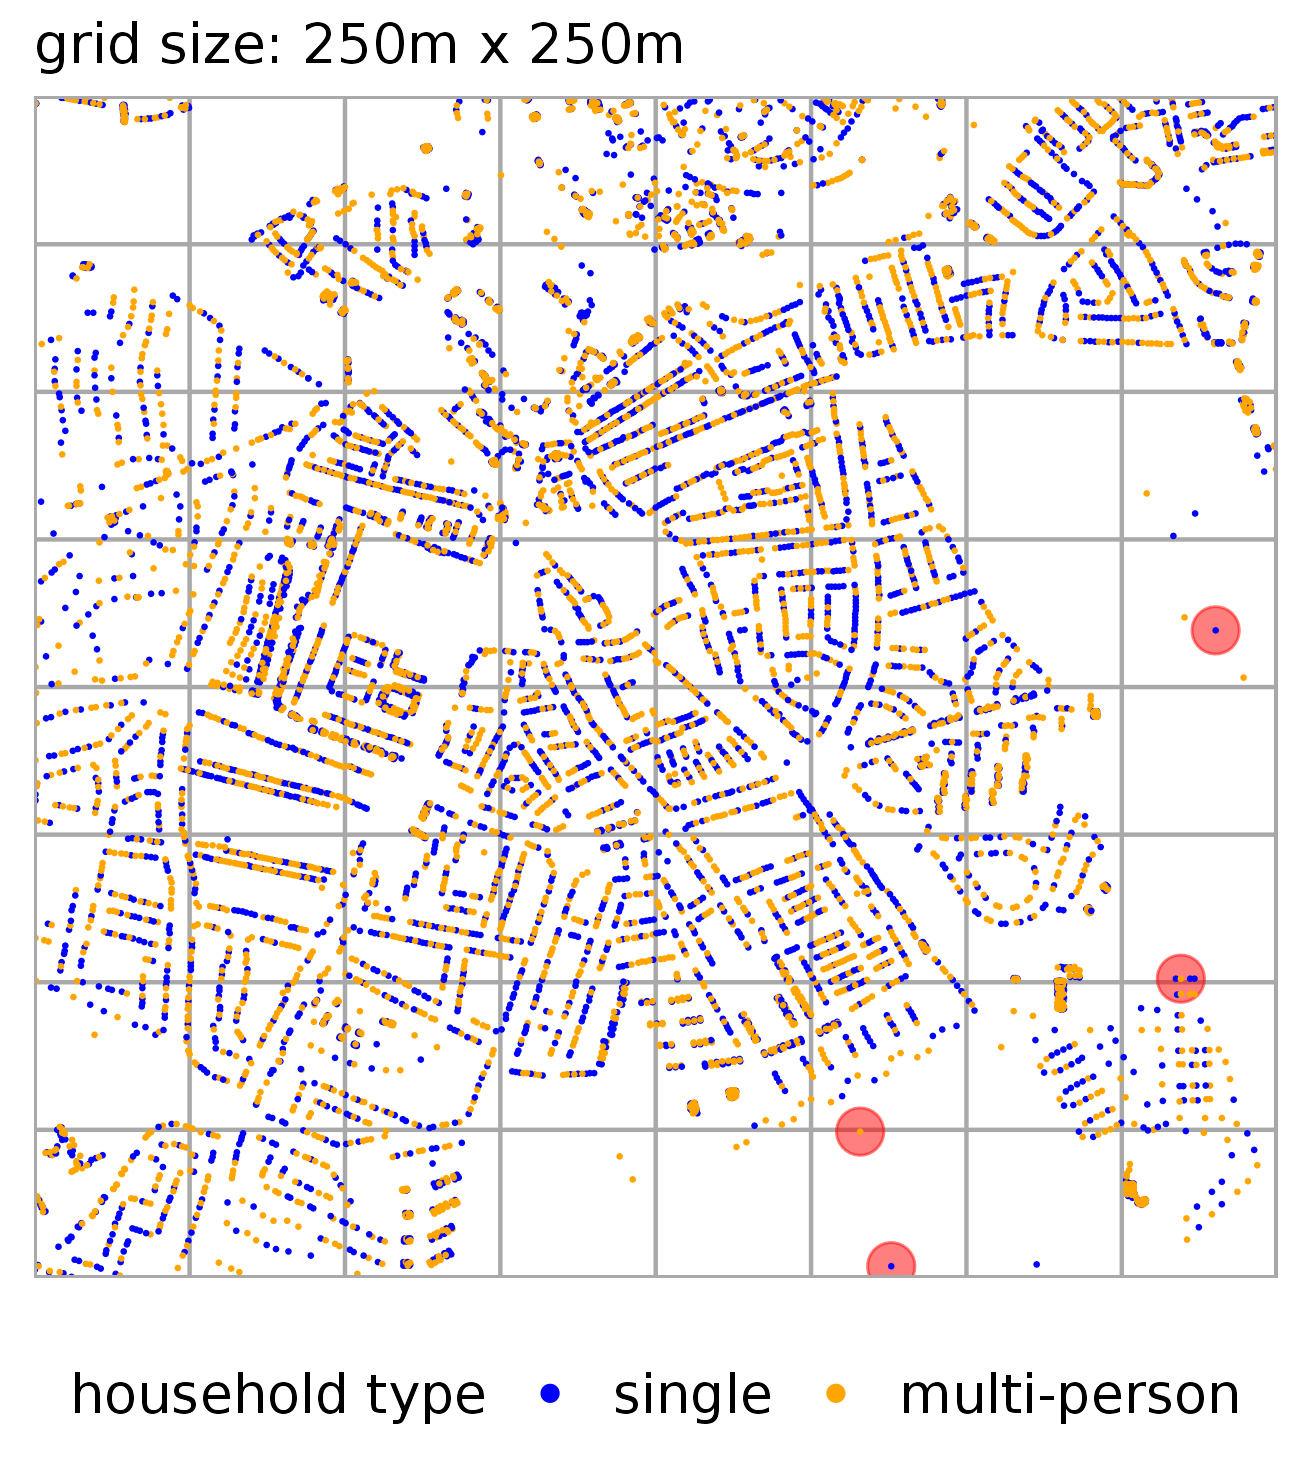
\includegraphics[width=0.495\linewidth]{figures/ExaMap_res1a.png}
    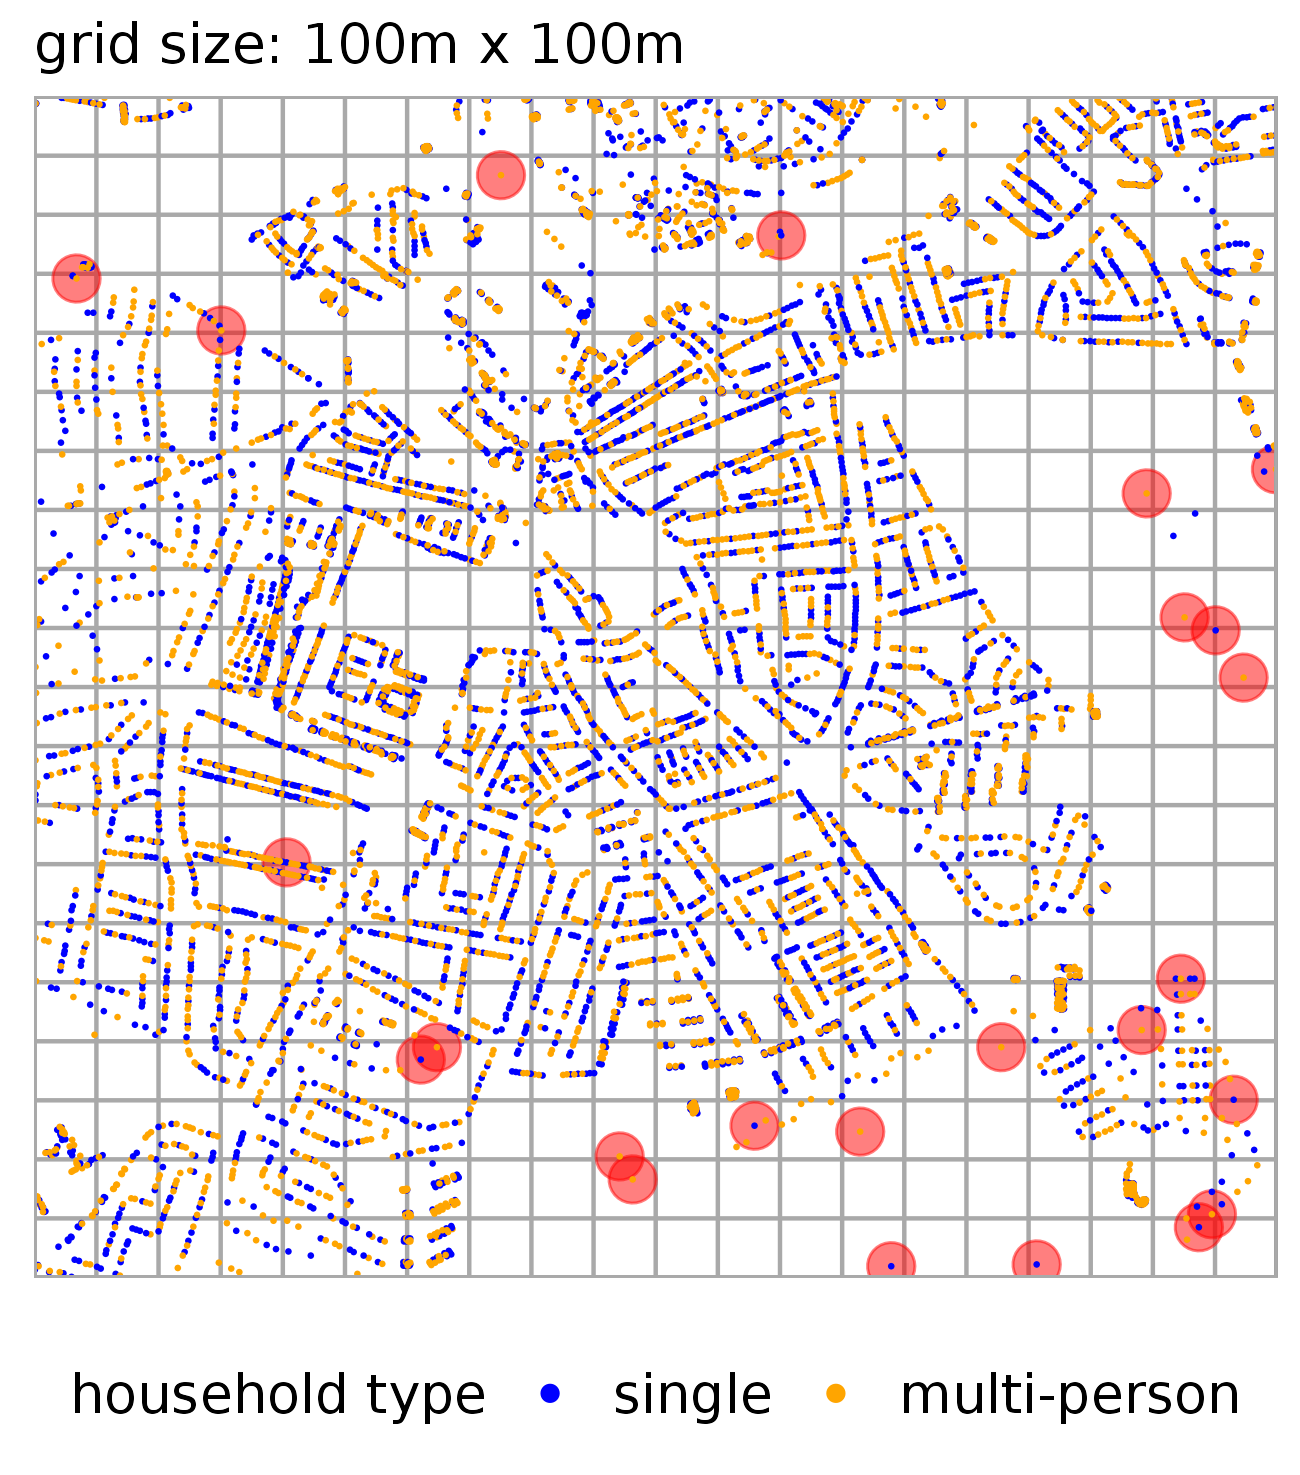
\includegraphics[width=0.495\linewidth]{figures/ExaMap_res1b.png}
    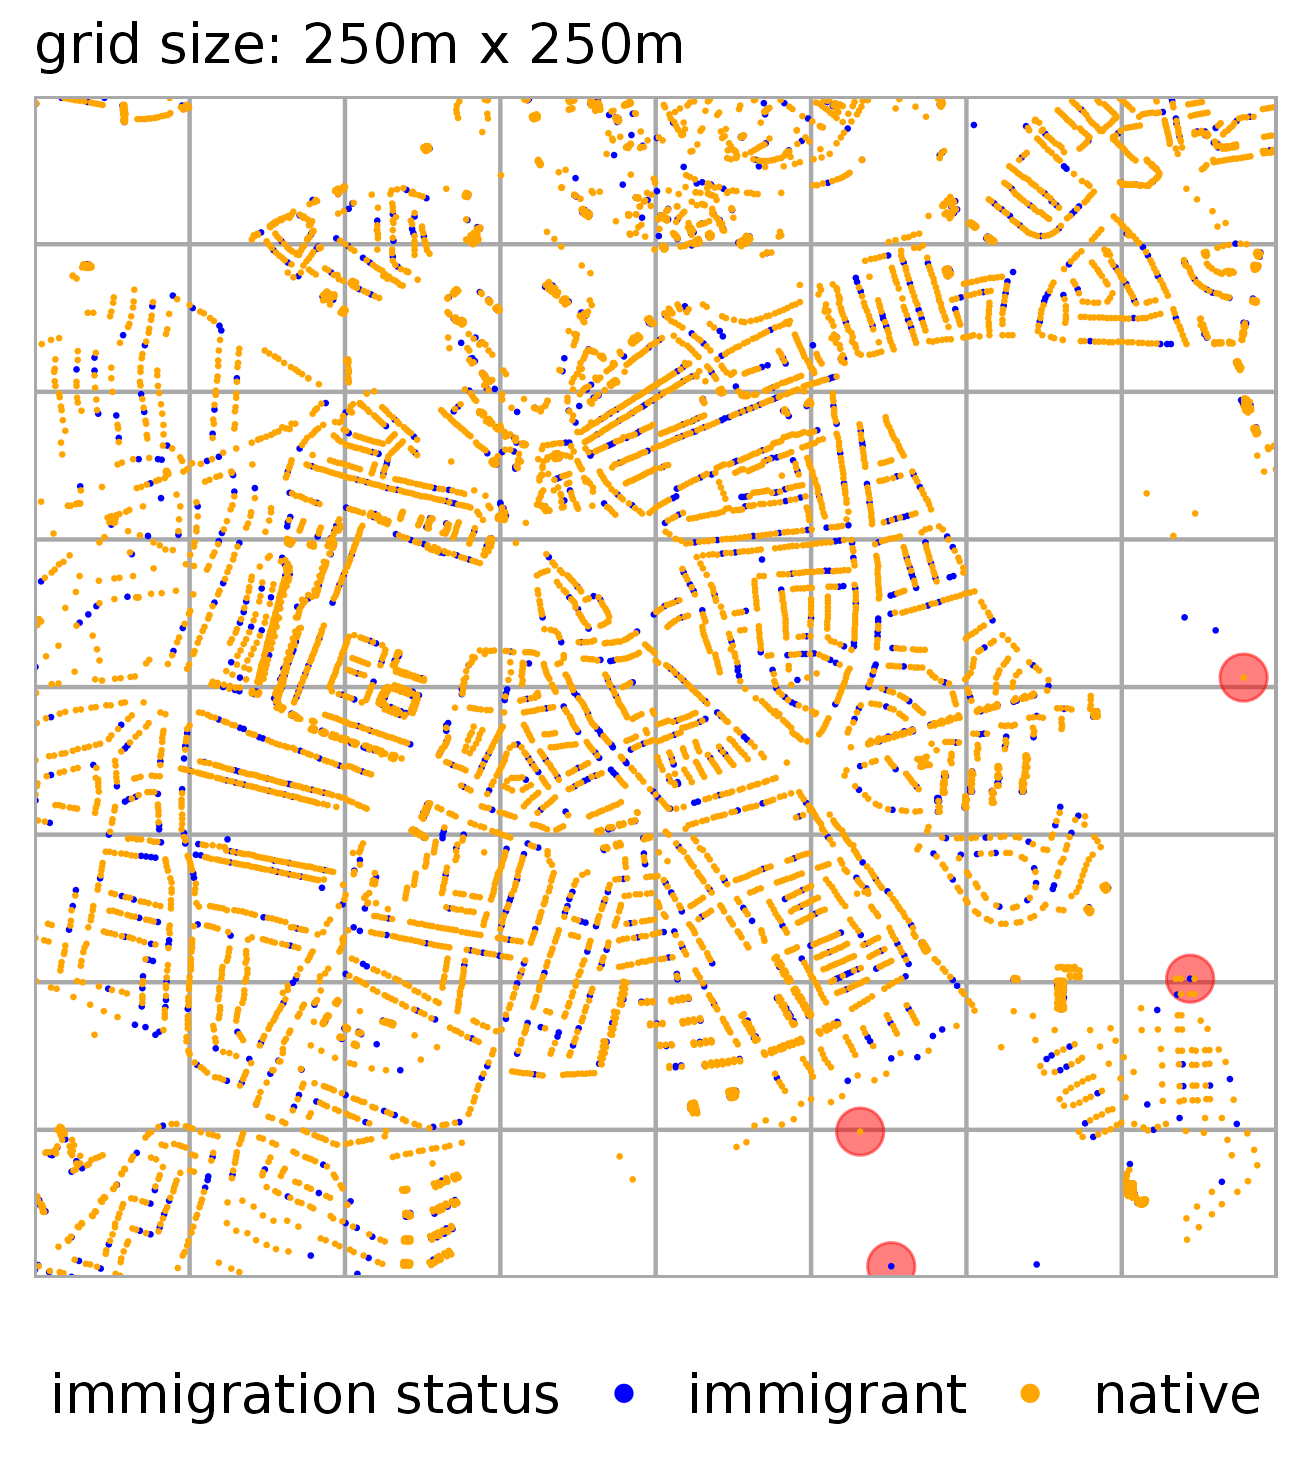
\includegraphics[width=0.495\linewidth]{figures/ExaMap_res2a.png}
    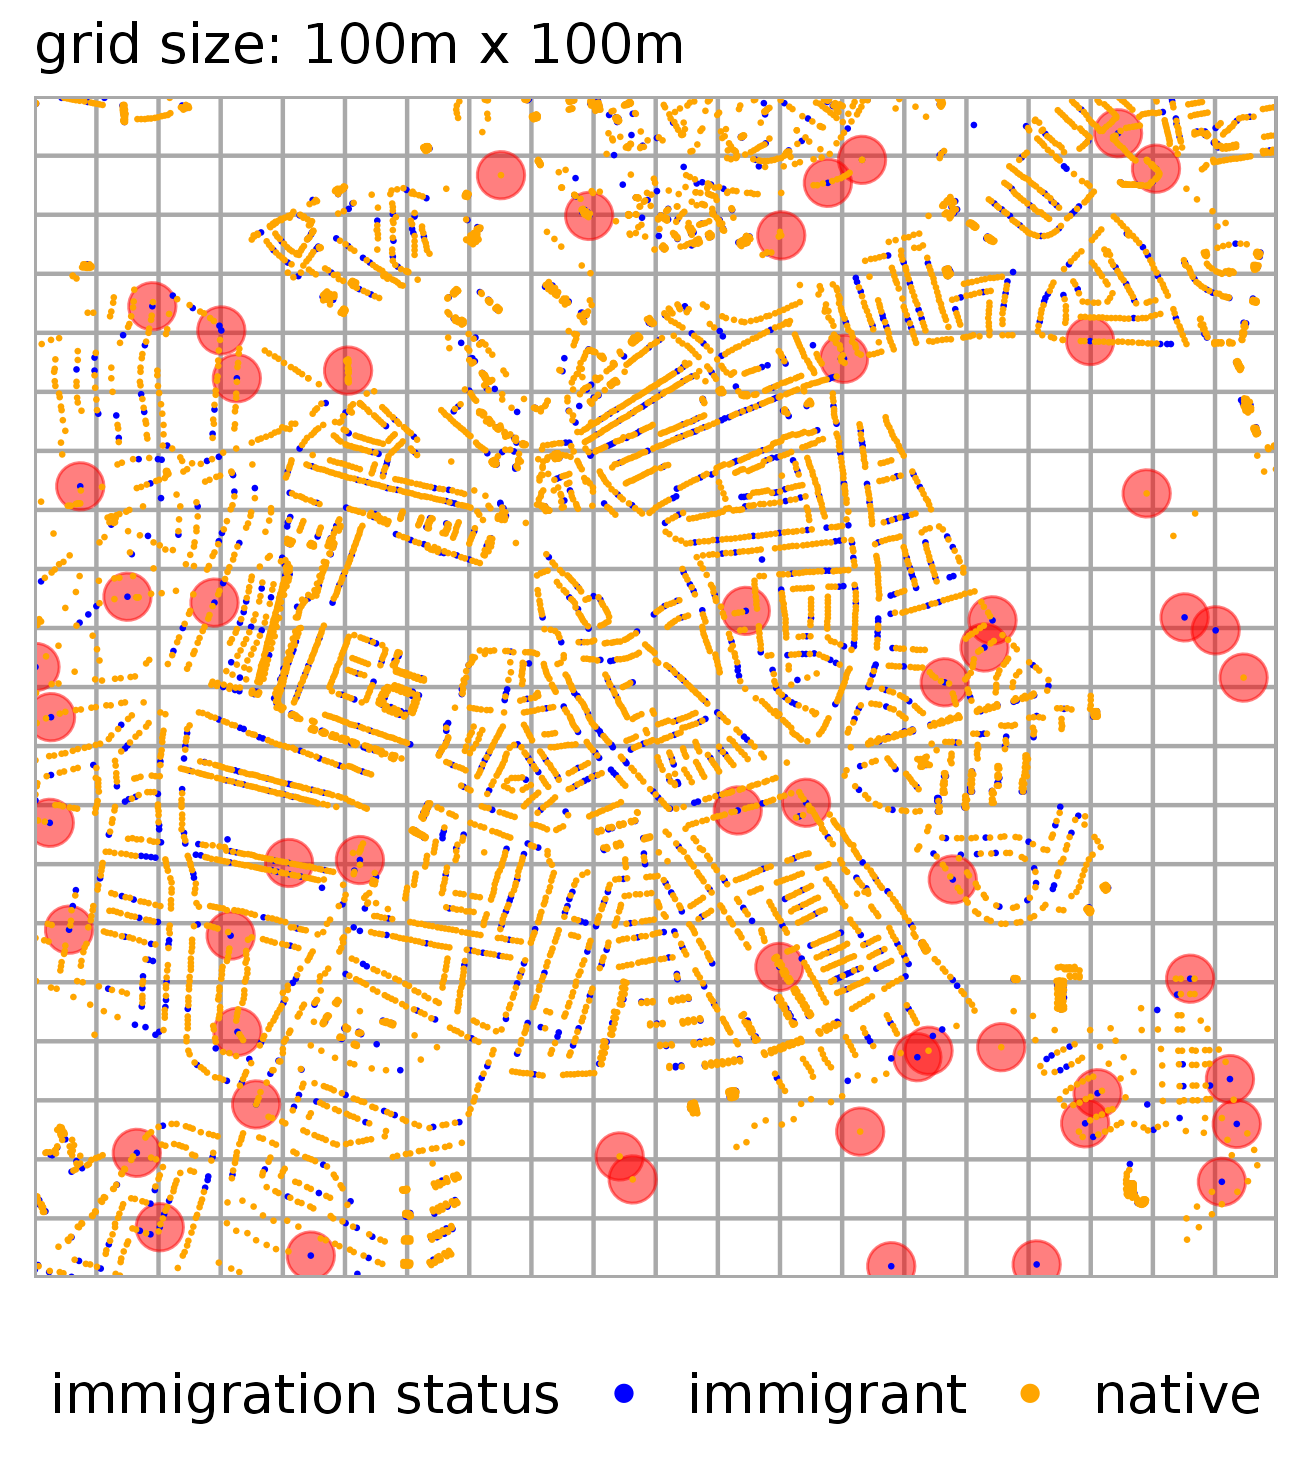
\includegraphics[width=0.495\linewidth]{figures/ExaMap_res2b.png}
    \caption{Fictitious maps of households by attribute `household type' (top) or `immigration status' (bottom), overlayed with geographic grid cells of size 250m $\times$ 250m (left) or 100m $\times$ 100m (right); marked in red are all households that would be uniquely identified by the cross-tabulation of grid cell and attribute.}
    \label{fig:ExaResMaps}
\end{figure}

The graph in Fig. \ref{fig:ExaResGraph} shows the number of aggregates that would only result in a single observation (count of 1) as a function of grid cell size. It illustrates that, generally speaking, \textit{the higher the level of detail in the geo-reference, the higher the expected risk of disclosure, especially for rare attributes}.\footnote{
    Note that we considered here attributes with only two categories. With more categories in the attribute, the issue would quickly be exacerbated further. The same is true when we add a third or fourth variable to the analysis. Incidentally, with a grid size of 100m $\times$ 100m, a 3-way aggregation of grid cell $\times$ household type $\times$ immigration status would leave 134 households identifiable, more than twice as many as in the most sensitive 2-way aggregation.
}
\begin{figure}
    \centering
    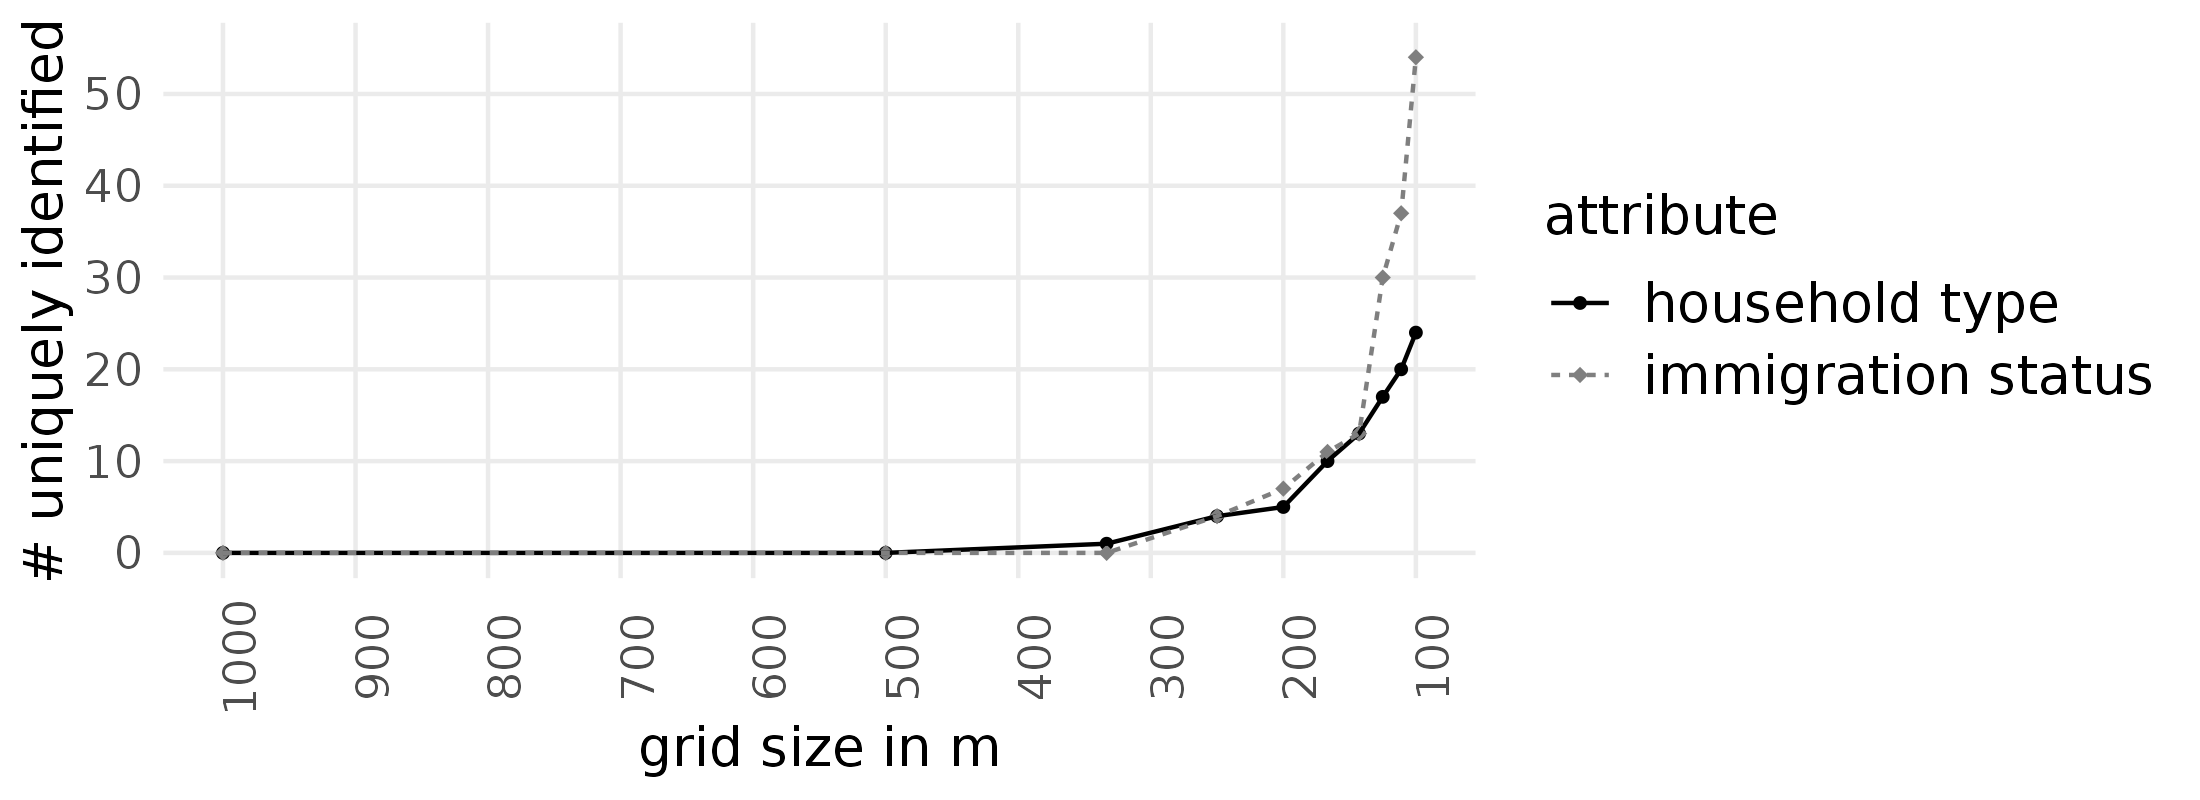
\includegraphics[width=\linewidth]{figures/ExaGraph_res2.png}
    \caption{No. of households from Fig. \ref{fig:ExaResMaps} uniquely identified by grid cell and attribute value as a function of cell size.}
    \label{fig:ExaResGraph}
\end{figure}

%\begin{figure}[H]
%    \centering
%    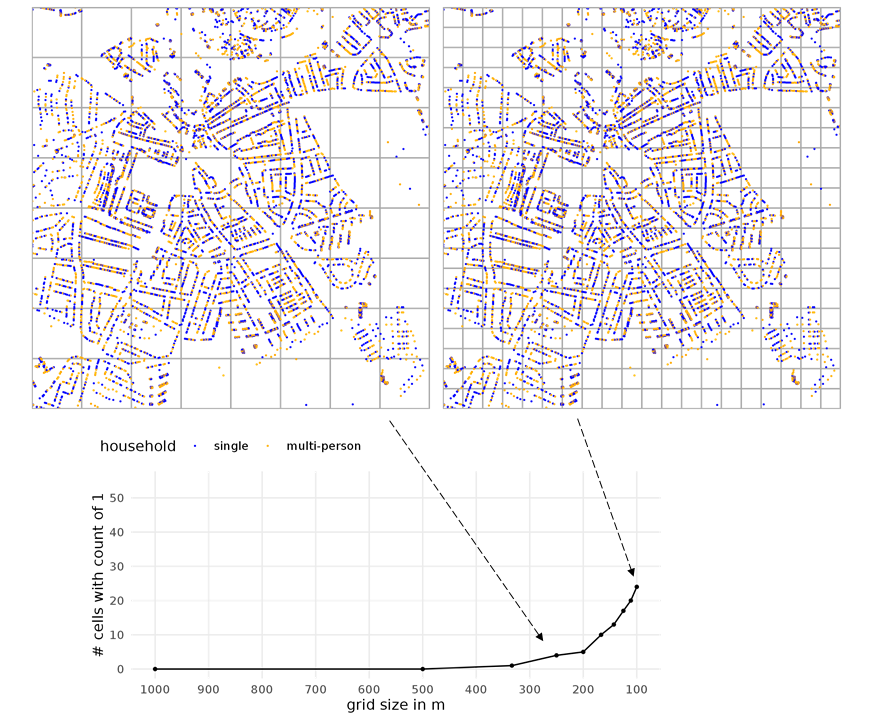
\includegraphics[width=\linewidth]{figures/ExaRes1.png}
%    \caption{Maps of households by type and grid cell (top); left: 250m $\times$ 250m grid, right: 100m $\times$ 100m grid; below: no. of households uniquely identified by grid cell and household type as a function of cell size.}
%    \label{fig:ExaRes1}
%\end{figure}

%\begin{figure}[H]
%    \centering
%    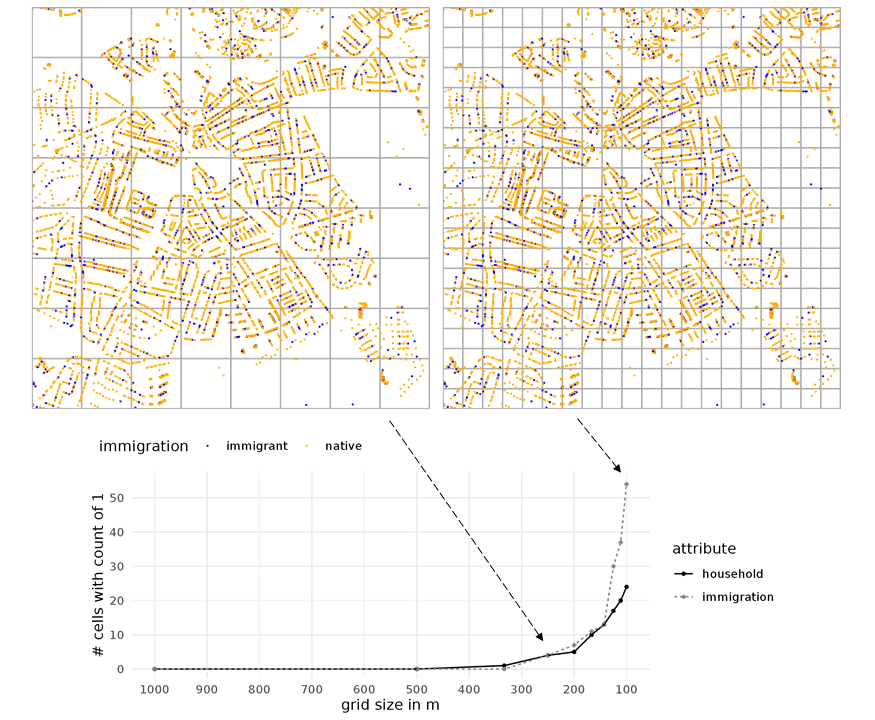
\includegraphics[width=\linewidth]{figures/ExaRes2.png}
%    \caption{Maps of households by immigration status and grid cell (top); left: 250m $\times$ 250m grid, right: 100m $\times$ 100m grid; below: no. of households uniquely identified by grid cell and immigration status as a function of cell size (graph from Fig. \ref{fig:ExaRes1} for reference).}
%    \label{fig:ExaRes2}
%\end{figure}

\subsection{The role of geographical characteristics of populations} \label{sec:ident_geochar}

\subsubsection{Population density and clustered versus disperse populations}

The (overall) population density is the total count of statistical units divided by the total size of the geographical space of interest. Generally speaking, the higher the population density, the more detailed the geo-reference can be, while still including enough units for each area and non-spatial attribute value to prevent disclosure problems. Likewise, for a given size of a geo-reference, the risk of disclosure tends to be higher in low-density compared to high-density regions. However, the total number of observations over a given geographical space can be a somewhat misleading indicator, since in reality population density is strongly heterogeneous. Therefore, one further needs to consider the local clustering characteristics of the population of interest.

\emph{Clustering} denotes the tendency of statistical units to crowd together in space. Consider the two populations of households mapped in Fig. \ref{fig:ExaDispClus} as dots. The one on the left sticks closely together, forming a heap or \emph{cluster}. The one on the right, on the other hand, disperses over the map much more consistently. Both patterns can be found in practice: the left one is typical for towns and cities, whereas the right one can sometimes be found in rural regions, for instance where households form farmsteads with surrounding arable land.
Clusters can provide a natural form of protection, as units blend together in dense centers, such as areas no. 6, 7, 10, and 11 in Fig. \ref{fig:ExaDispClus} (left). However, at the margins of settlements and in rural regions, where units are spaced more loosely, disclosure problems often arise. This is illustrated in Table \ref{tab:ExaDispClus}.

\begin{figure}[H]
    \centering
    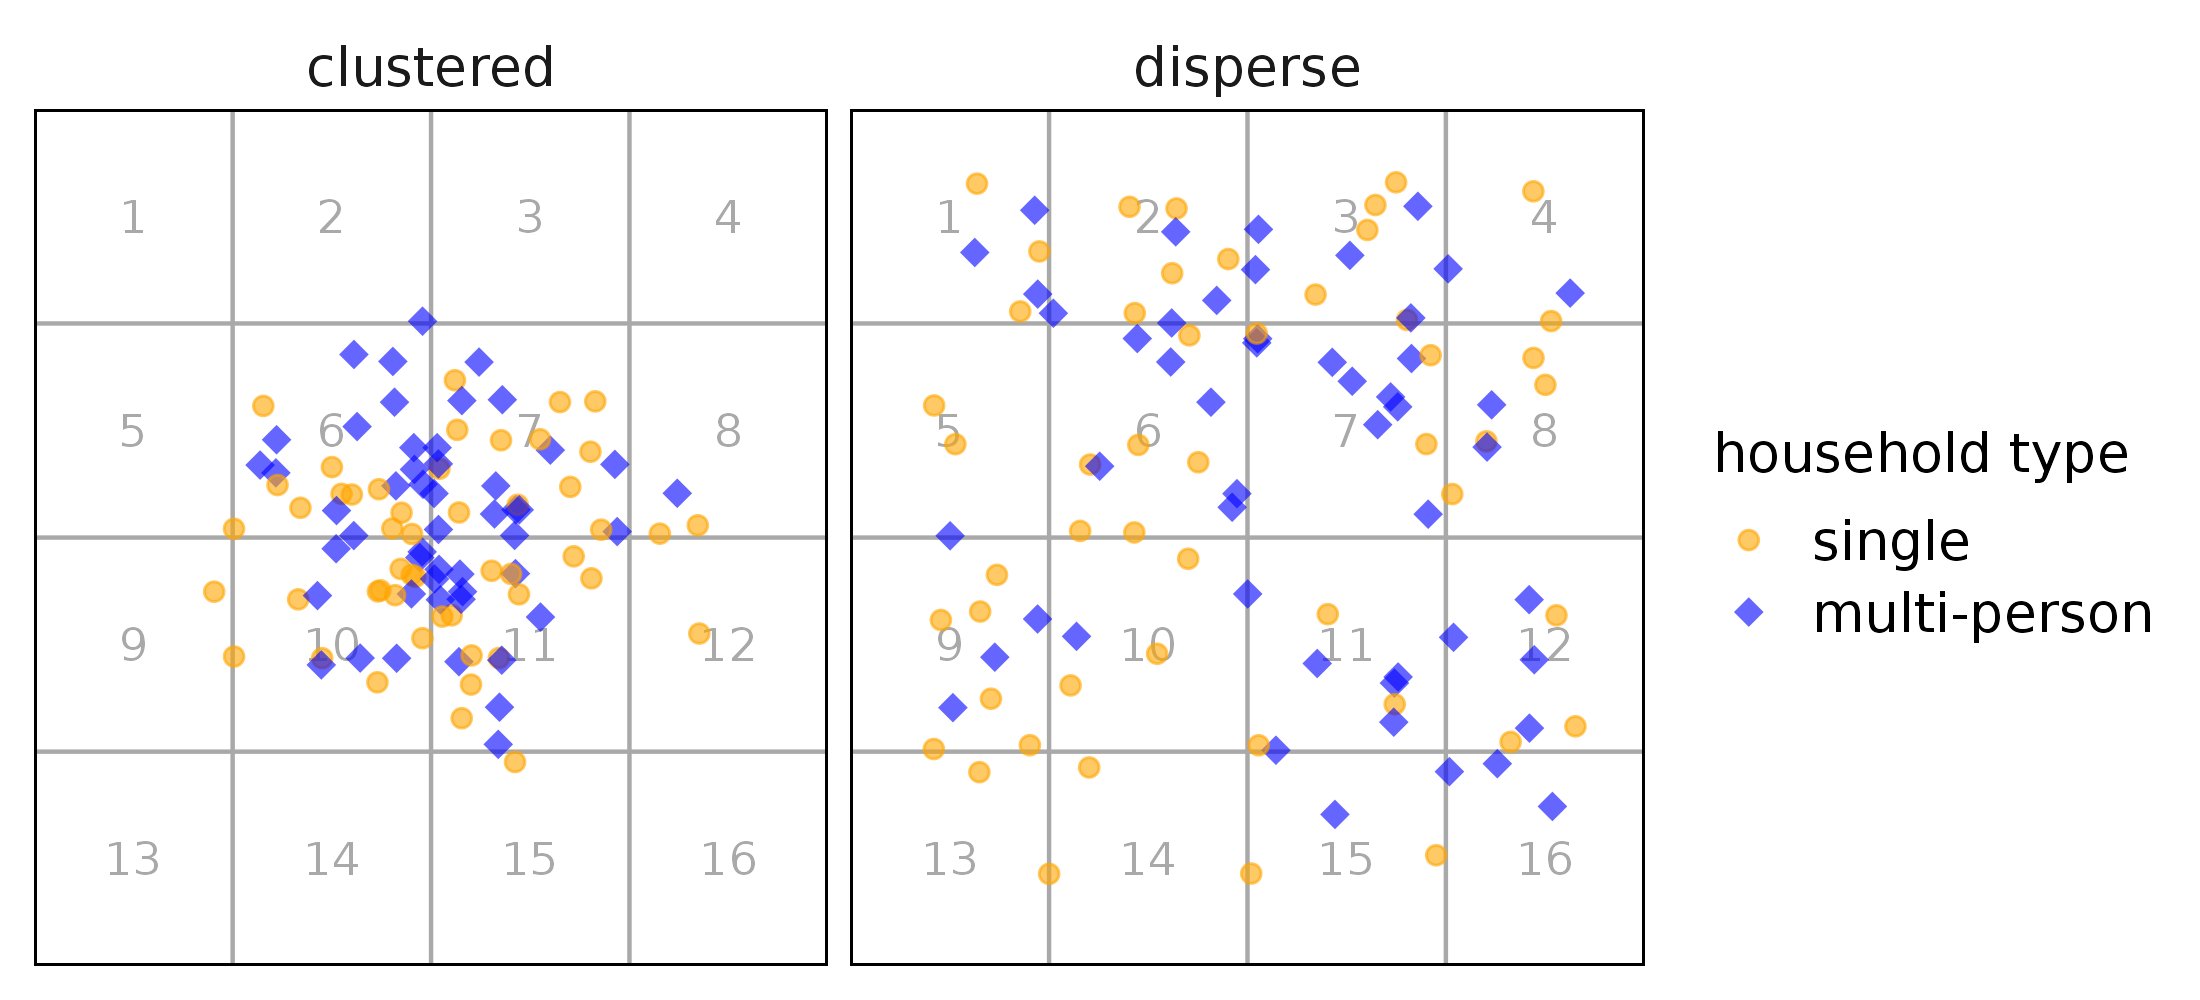
\includegraphics[width=\linewidth]{figures/ExaMap_clus_disp.png}
    \caption{Two artificial populations of the same size ($N = 100$), displaying different geographic characteristics: left clustered, right disperse; both are additionally classified by an attribute variable (household type); sub-areas of the map are numbered 1-16.}
    \label{fig:ExaDispClus}
\end{figure}

\begin{table}[H]
    \centering
    \begin{tabular}{|l|cc|c|  c  |l|cc|c|}
        \multicolumn{4}{c}{\emph{clustered}} & \multicolumn{1}{c}{} & \multicolumn{4}{c}{\emph{disperse}}\\[7pt]
        \cline{1-4} \cline{6-9}
        \multirow{2}{*}{area} & \multicolumn{2}{c|}{household type} & \multirow{2}{*}{total} & &
        \multirow{2}{*}{area} & \multicolumn{2}{c|}{household type} & \multirow{2}{*}{total}\\[5pt]
         & single & multi & & & & single & multi & \\
        \cline{1-4} \cline{6-9}
        1  & -  & -  & -  &  & 1  & \textcolor{blue}{3} & \textcolor{blue}{3} & 6  \\
        2  & -  & \textcolor{red}{1}  & \textcolor{red}{1}  &  & 2  & 5 & \textcolor{blue}{4} & 9  \\
        3  & -  & -  & -  &  & 3  & 5 & 5 & 10 \\
        4  & -  & -  & -  &  & 4  & \textcolor{red}{2} & \textcolor{red}{2} & \textcolor{blue}{4}  \\
        5  & -  & -  & -  &  & 5  & \textcolor{red}{2} & \textcolor{red}{1} & \textcolor{blue}{3}  \\
        6  & 11 & 13 & 24 &  & 6  & 6 & 6 & 12 \\
        7  & 12 & 15 & 27 &  & 7  & \textcolor{blue}{3} & 9 & 12 \\
        8  & \textcolor{red}{2}  & \textcolor{red}{1}  & \textcolor{blue}{3}  &  & 8  & \textcolor{blue}{4} & \textcolor{red}{2} & 6  \\
        9  & \textcolor{red}{1}  & -  & \textcolor{red}{1}  &  & 9  & 6 & \textcolor{blue}{3} & 9  \\
        10 & 11 & 8  & 19 &  & 10 & \textcolor{blue}{3} & \textcolor{red}{1} & \textcolor{blue}{4}  \\
        11 & 11 & 12 & 23 &  & 11 & \textcolor{blue}{3} & 6 & 9  \\
        12 & \textcolor{red}{1}  & -  & \textcolor{red}{1}  &  & 12 & \textcolor{blue}{3} & \textcolor{blue}{4} & 7  \\
        13 & -  & -  & -  &  & 13 & \textcolor{red}{1} & - & \textcolor{red}{1}  \\
        14 & -  & -  & -  &  & 14 & \textcolor{red}{2} & - & \textcolor{red}{2}  \\
        15 & \textcolor{red}{1}  & -  & \textcolor{red}{1}  &  & 15 & \textcolor{red}{2} & \textcolor{red}{1} & \textcolor{blue}{3}  \\
        16 & -  & -  & -  &  & 16 & - & \textcolor{blue}{3} & \textcolor{blue}{3}  \\
        \cline{1-4} \cline{6-9}
        \cline{1-4} \cline{6-9}
        total & 50 & 50 & 100 & & total & 50 & 50 & 100\\ 
        \cline{1-4} \cline{6-9}
    \end{tabular}
    \caption{Tabular representation of Fig. \ref{fig:ExaDispClus} data; cells in red are sensitive, when a minimum frequency rule of 3 is used, cells in blue are additionally sensitive, when a minimum frequency rule of 5 is used.}
    \label{tab:ExaDispClus}
\end{table}

%\begin{table}[H]
%    \centering
%    \begin{tabular}{|l|cc|c|  c  |l|cc|c|}
%        \multicolumn{4}{c}{\emph{clustered}} & \multicolumn{1}{c}{} & \multicolumn{4}{c}{\emph{disperse}}\\[7pt]
%        \cline{1-4} \cline{6-9}
%        \multirow{2}{*}{area} & \multicolumn{2}{c|}{household type} & \multirow{2}{*}{total} & &
%        \multirow{2}{*}{area} & \multicolumn{2}{c|}{household type} & \multirow{2}{*}{total}\\[5pt]
%         & single & multi & & & & single & multi & \\
%        \cline{1-4} \cline{6-9}
%        1  & -  & -  & -  &  & 1  & \textcolor{blue}{3} & \textcolor{blue}{3} & 6  \\
%        2  & -  & \cellcolor{lgrey}\textcolor{red}{1}  & \cellcolor{lgrey}\textcolor{red}{1}  &  & 2  & 5 & \textcolor{blue}{4} & 9  \\
%        3  & -  & -  & -  &  & 3  & 5 & 5 & 10 \\
%        4  & -  & -  & -  &  & 4  & \textcolor{red}{2} & \textcolor{red}{2} & \textcolor{blue}{4}  \\
%        5  & -  & -  & -  &  & 5  & \textcolor{red}{2} & \textcolor{red}{1} & \textcolor{blue}{3}  \\
%        6  & 11 & 13 & 24 &  & 6  & 6 & 6 & 12 \\
%        7  & 12 & 15 & 27 &  & 7  & \textcolor{blue}{3} & 9 & 12 \\
%        8  & \textcolor{red}{2}  & \textcolor{red}{1}  & \textcolor{blue}{3}  &  & 8  & \textcolor{blue}{4} & \textcolor{red}{2} & 6  \\
%        9  & \cellcolor{lgrey}\textcolor{red}{1}  & \cellcolor{lgrey}-  & \cellcolor{lgrey}\textcolor{red}{1}  &  & 9  & 6 & \textcolor{blue}{3} & 9  \\
%        10 & 11 & 8  & 19 &  & 10 & \textcolor{blue}{3} & \textcolor{red}{1} & \textcolor{blue}{4}  \\
%        11 & 11 & 12 & 23 &  & 11 & \textcolor{blue}{3} & 6 & 9  \\
%        12 & \cellcolor{lgrey}\textcolor{red}{1}  & \cellcolor{lgrey}-  & \cellcolor{lgrey}\textcolor{red}{1}  &  & 12 & \textcolor{blue}{3} & \textcolor{blue}{4} & 7  \\
%        13 & -  & -  & -  &  & 13 & \cellcolor{lgrey}\textcolor{red}{1} & \cellcolor{lgrey}- & \cellcolor{lgrey}\textcolor{red}{1}  \\
%        14 & -  & -  & -  &  & 14 & \cellcolor{lgrey}\textcolor{red}{2} & \cellcolor{lgrey}- & \cellcolor{lgrey}\textcolor{red}{2}  \\
%        15 & \cellcolor{lgrey}\textcolor{red}{1}  & \cellcolor{lgrey}-  & \cellcolor{lgrey}\textcolor{red}{1}  &  & 15 & \textcolor{red}{2} & \textcolor{red}{1} & \textcolor{blue}{3}  \\
%        16 & -  & -  & -  &  & 16 & \cellcolor{lgrey}- & \cellcolor{lgrey}\textcolor{blue}{3} & \cellcolor{lgrey}\textcolor{blue}{3}  \\
%        \cline{1-4} \cline{6-9}
%        \cline{1-4} \cline{6-9}
%        total & 50 & 50 & 100 & & total & 50 & 50 & 100\\ 
%        \cline{1-4} \cline{6-9}
%    \end{tabular}
%    \caption{Tabular representation of Fig. \ref{fig:ExaDispClus} data; cells in red are sensitive, when a minimum frequency rule of 3 is used, cells in blue are additionally sensitive, when a minimum frequency rule of 5 is used. Grey rows are vulnerable to attribute disclosure \citep[5.2]{HundepoolEtAl2024}.
%    }
%    \label{tab:ExaDispClus}
%\end{table}

Table \ref{tab:ExaDispClus} is the frequency table representation of Fig. \ref{fig:ExaDispClus}. It is derived by cross-tabulating the area identifier (1-16) with household type (single or multi-person). For risk assessment we assume a frequency rule (see section \ref{sec:risk_aggr_geosp}), where a table cell is considered unsafe, if it contains fewer units than a certain threshold (here: 3 or 5). 
When comparing the two tables side by side, it becomes clear that the level of protection a \emph{clustered} population provides varies widely: units in the dense center enjoy strong protection, whereas units at the margin can be unsafe. 
In the case of a \emph{disperse} population, the distribution of counts is much more even and hence the risk of small cell counts is more widespread.

\subsubsection{Attribute clustering and `sticky' populations}

Following \cite{ElliotEtAl1998}, the concept of a `sticky' population means the tendency of statistical units to form geographical clusters according to their attributes. For instance, suppose we assign to each household in a large area one of 5 categories, depending on where it stands on the income ladder (richest 20\%, next-richest 20\% etc., all the way to the poorest 20\%). If we now look at a smaller subregion, do we expect all categories to appear with equal frequency? This is usually not the case, as people of some income category are likely to live in neighborhoods with others of the same category.

Such a clustering tendency can be assumed for some, but not for all variables that may be potentially identifying. For example, while the category of household income may be clustered, this is often not the case (or only to a small degree) for variables like age group or gender.\footnote{
    `Sticky' populations may be seen an application of \emph{Tobler's Law}, variously known is the \emph{First Law of Geography}, a heuristic by which interaction (and hence often correlation in attributes) is stronger between things that are geographically close to one-another, rather than far apart. See e.g. \citet{Miller2004}.
}
There are two main implications for disclosure risk:
\begin{enumerate}
    \item For a sticky population, risk of \emph{identity disclosure} \cite[5.2]{HundepoolEtAl2024} tends to be smaller than for a non-sticky population. This is because attribute clustering decreases the variability of attributes within a region. Such lower variability in turn decreases the expected number of rare or unique attribute combinations \citep{GreenbergVoshell1990}. 
    \item At the same time - and for exactly the same reason - stickiness can increase the risk of \emph{attribute disclosure} \citep{BuronFontaine2018}. People with shared characteristics that require special protection (e.g. asylum status) also tend to cluster in space.
\end{enumerate}

By way of example, consider the two populations mapped in Fig. \ref{fig:ExaDispClus_sticky}. The placement is the same as in Fig. \ref{fig:ExaDispClus}, but the attribute variable is changed to show a clustering tendency. Table \ref{tab:ExaDispClus_sticky} is again the frequency table representation of Fig. \ref{fig:ExaDispClus_sticky} (tabulating household type by area).

\begin{figure}[H]
    \centering
    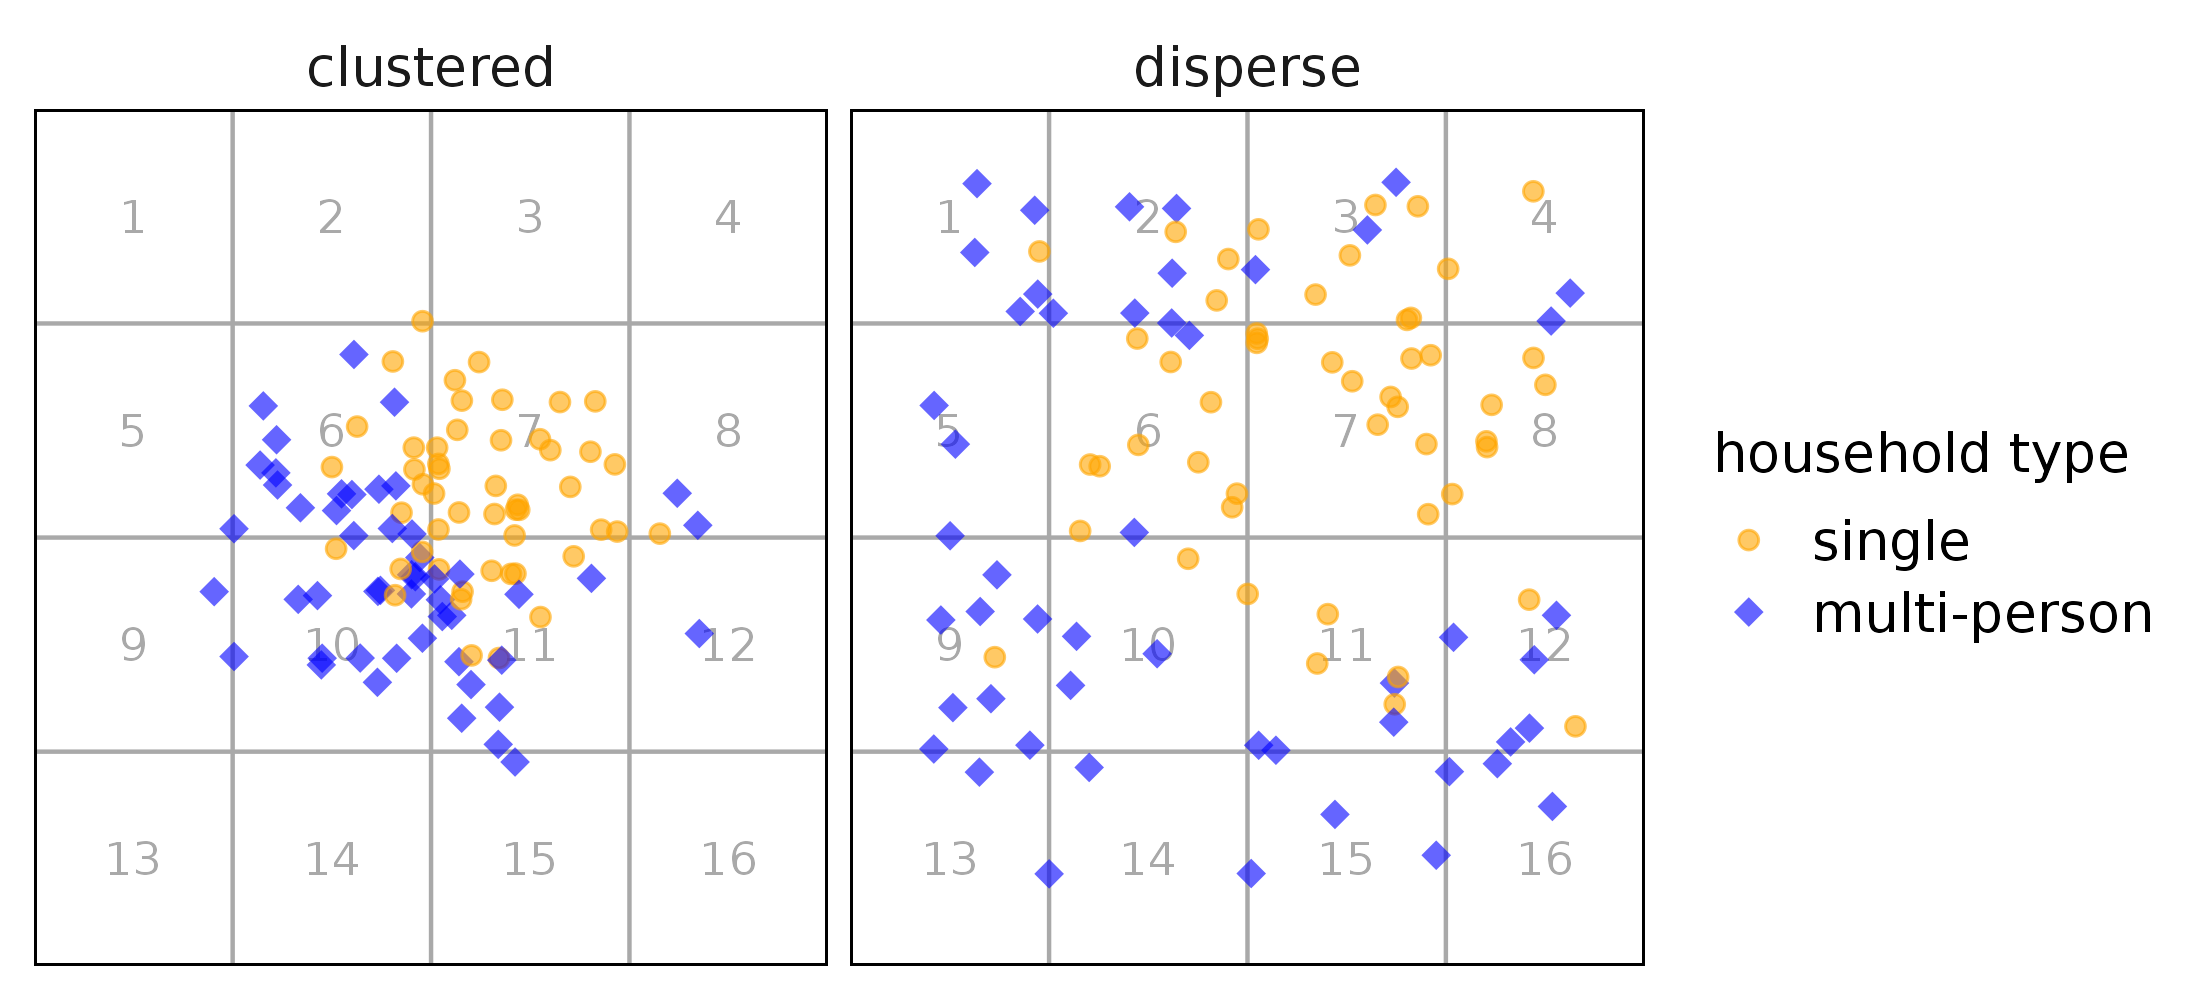
\includegraphics[width=\linewidth]{figures/ExaMap_clus_disp2.png}
    \caption{Alternative version of Fig. \ref{fig:ExaDispClus}, displaying attribute clustering. The sub-populations of single and multi-person households are `sticky', i.e. households with the same attribute tend to lump together spatially.}
    \label{fig:ExaDispClus_sticky}
\end{figure}

\begin{table}[H]
    \centering
    \begin{tabular}{|l|cc|c|  c  |l|cc|c|}
        \multicolumn{4}{c}{\emph{clustered}} & \multicolumn{1}{c}{} & \multicolumn{4}{c}{\emph{disperse}}\\[7pt]
        \cline{1-4} \cline{6-9}
        \multirow{2}{*}{area} & \multicolumn{2}{c|}{household type} & \multirow{2}{*}{total} & &
        \multirow{2}{*}{area} & \multicolumn{2}{c|}{household type} & \multirow{2}{*}{total}\\[5pt]
         & single & multi & & & & single & multi & \\
        \cline{1-4} \cline{6-9}
        1  & -  & -  & - &  & 1  & \textcolor{red}{1}  & 5 & 6  \\
        2  & \cellcolor{lgrey}\textcolor{red}{1}  & \cellcolor{lgrey}- & \cellcolor{lgrey}\textcolor{red}{1} &  & 2  & \textcolor{blue}{3}  & 6 & 9  \\
        3  & -  & -  & -  &  & 3  & 7  & \textcolor{blue}{3} & 10 \\
        4  & -  & -  & -  &  & 4  & \textcolor{red}{2}  & \textcolor{red}{2} & \textcolor{blue}{4}  \\
        5  & -  & -  & -  &  & 5  & \cellcolor{lgrey}-  & \cellcolor{lgrey}\textcolor{blue}{3} & \cellcolor{lgrey}\textcolor{blue}{3}  \\
        6  & 7  & 17 & 24 &  & 6  & 10 & \textcolor{red}{2} & 12 \\
        7  & \cellcolor{lgrey}27 & \cellcolor{lgrey}-  & \cellcolor{lgrey}27 &  & 7  & \cellcolor{lgrey}12 & \cellcolor{lgrey}- & \cellcolor{lgrey}12 \\
        8  & \textcolor{red}{1}  & \textcolor{red}{2}  & 3  &  & 8  & \cellcolor{lgrey}6  & \cellcolor{lgrey}- & \cellcolor{lgrey}6  \\
        9  & \cellcolor{lgrey}- & \cellcolor{lgrey}\textcolor{red}{1}  & \cellcolor{lgrey}\textcolor{red}{1}  &  & 9  & \textcolor{red}{1}  & 8 & 9  \\
        10 & \textcolor{blue}{4}  & 15 & 19 &  & 10 & \textcolor{red}{1}  & \textcolor{blue}{3} & \textcolor{blue}{4}  \\
        11 & 10 & 13 & 23 &  & 11 & 5  & \textcolor{blue}{4} & 9  \\
        12 & \cellcolor{lgrey}-  & \cellcolor{lgrey}\textcolor{red}{1}  & \cellcolor{lgrey}\textcolor{red}{1}  &  & 12 & \textcolor{red}{2}  & 5 & 7  \\
        13 & -  & -  & -  &  & 13 & \cellcolor{lgrey}-  & \cellcolor{lgrey}\textcolor{red}{1} & \cellcolor{lgrey}\textcolor{red}{1}  \\
        14 & -  & -  & -  &  & 14 & \cellcolor{lgrey}-  & \cellcolor{lgrey}\textcolor{red}{2} & \cellcolor{lgrey}\textcolor{red}{2}  \\
        15 & \cellcolor{lgrey}-  & \cellcolor{lgrey}\textcolor{red}{1}  & \cellcolor{lgrey}\textcolor{red}{1}  &  & 15 & \cellcolor{lgrey}-  & \cellcolor{lgrey}\textcolor{blue}{3} & \cellcolor{lgrey}\textcolor{blue}{3}  \\
        16 & -  & -  & -  &  & 16 & \cellcolor{lgrey}-  & \cellcolor{lgrey}\textcolor{blue}{3} & \cellcolor{lgrey}\textcolor{blue}{3}  \\
        \cline{1-4} \cline{6-9}
        \cline{1-4} \cline{6-9}
        total & 50 & 50 & 100 & & total & 50 & 50 & 100\\ 
        \cline{1-4} \cline{6-9}
    \end{tabular}
    \caption{Tabular representation of Fig. \ref{fig:ExaDispClus_sticky} data; cells in red are sensitive, when a minimum frequency rule of 3 is used, cells in blue are additionally sensitive, when a minimum frequency rule of 5 is used. Grey rows are vulnerable to attribute disclosure \citep[5.2]{HundepoolEtAl2024}.}
    \label{tab:ExaDispClus_sticky}
\end{table}

Compare Table \ref{tab:ExaDispClus_sticky} to Table \ref{tab:ExaDispClus}. For the clustered population, the switch to sticky populations did not change the number of table cells that fall below the frequency threshold. However, 31 units are now at risk of (group) attribute disclosure. Most notably, it is disclosed that whenever a household is located in area 7, it is a single person household. The corresponding number of units at risk of attribute disclosure in Table \ref{tab:ExaDispClus} (left) was 4.
Comparing the situation for the disperse population, we can see that the number of small cells that may pose a risk of identity disclosure is slightly lower (11 vs. 12 for the threshold of 3 and 12 vs. 16 for the threshold of 5). The number of units at risk of attribute disclosure has risen from 6 to 30.\\

In general, a clustering tendency for identifying variables can be helpful for avoiding disclosure, as it will tend to reduce the likelihood of rare attribute combinations. A clustering tendency for sensitive attributes, for which attribute disclosure is to be avoided, can be a challenge.

\section{Outputs based on geo-referenced data}

Geo-referenced data can be the basis for a variety of outputs. \emph{Microdata files} and \emph{aggregate tables} 
%(of frequencies or magnitudes) 
are the classical products of statistical offices.
%; see \citet[~p.7]{HundepoolEtAl2010}. 
With the inclusion of the spatial domain, detailed \emph{thematic maps} are added, which can be static (for print) or interactive (for digital publication). Maps often add analytical value over mere tabulations of spatial data; see, for instance, \citet{Waller2024}.
Fig. \ref{fig:rep_map} shows people aged 65 or above in a rural region, geo-referenced to grid cells of size 1km $\times$ 1km. Tables \ref{tab:rep_tab} and \ref{tab:rep_micro} present the same ground truth as alternative representations, once as frequency table and once as microdata table.

Typically all these outputs need to be protected and if one and the same data is used for two or all three types, it would be best if the protection is consistent across them. This is facilitated by an underlying equivalence: Fig. \ref{fig:rep_map} is a visualization of table \ref{tab:rep_tab}, which in turn tabulates micro data table \ref{tab:rep_micro}.
Some methods of disclosure control, like the Cell Key Method (see section \ref{sec:ckm}), therefore protect the map by protecting the table. Others, like Targeted record swapping (see section \ref{sec:trs}), act on the micro data to protect the tables and maps derived from it. Still others, like spatial smoothing (see section \ref{sec:methods_smooth}), consider the map an output product in its own right and aim to protect it specifically.

\newpage

% Map centered around ca. lat 6.33, lon 51.63 in Web Mercator (R package mapView); betw. Kervenheim and Sonsbeck, SE of Kleve (NW), Germany, near the border to Netherlands; grid definition in ETRS89 LAEA
\begin{figure}[H]
    \centering
    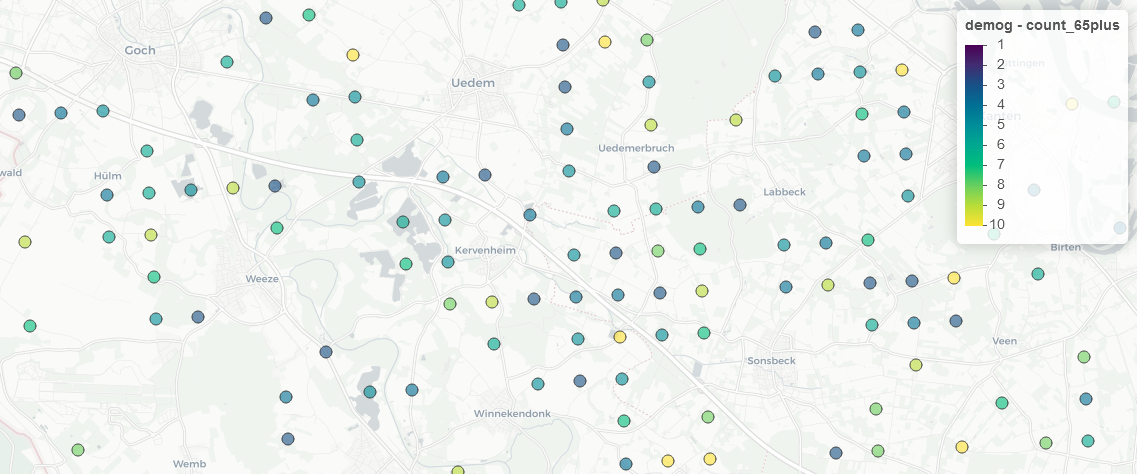
\includegraphics[width=\linewidth]{figures/rep_map.png}
    \caption{\emph{Map} representation of geo-referenced data (no. of inhabitants aged 65+ in 1km$^2$ grid cells); each colored marker equates to a table cell in aggregate table \ref{tab:rep_tab} and a block of entries in microdata table \ref{tab:rep_micro}.}
    \label{fig:rep_map}
\end{figure}

\begin{table}[H]
    \centering
    \begin{tabular}{c | c c c c c}
         \multirow{2}*{Northing} & \multicolumn{4}{c}{Easting} &\\
         & E:4065 & E:4066 & E:4067 & E:4068 & \ldots \\
         \hline
         N:3176 & - & 6 & 3 & 4 & \multirow{3}*{$\cdots$}\\
         N:3175 & 5 & 3 & 8 & 7 &\\
         N:3174 & 4 & 4 & 3 & 9 &\\
         \vdots & \multicolumn{4}{c}{\vdots} & $\ddots$
    \end{tabular}
    \caption{\emph{Table} representation of geo-referenced data (no. of inhabitants aged 65+ in 1km$^2$ grid cells), each table cell equates to a colored marker in map Fig. \ref{fig:rep_map} and a block of entries in microdata table \ref{tab:rep_micro}.}
    \label{tab:rep_tab}
\end{table}

\begin{table}[H]
    \centering
    \begin{tabular}{c c c}
         unit ID & grid cell ID & age group \\
         \hline
         1 & N:3176 E:4066 & 65+ \\
         2 & N:3176 E:4066 & 65+ \\
         3 & N:3176 E:4066 & 65+ \\
         4 & N:3176 E:4066 & 65+ \\
         5 & N:3176 E:4066 & 65+ \\
         6 & N:3176 E:4066 & 65+ \\
         7 & N:3176 E:4067 & 65+ \\
         8 & N:3176 E:4067 & 65+ \\
         9 & N:3176 E:4067 & 65+ \\
         \multicolumn{3}{c}{$\vdots$}
    \end{tabular}
    \caption{\emph{Microdata} representation of geo-referenced data (inhabitants aged 65+ in 1km$^2$ grid cells); each block of entries with same grid cell ID equates to  a colored marker in map Fig. \ref{fig:rep_map} and a table cell in aggregate table \ref{tab:rep_tab}.}
    \label{tab:rep_micro}
\end{table}



\chapter{Measuring Disclosure Risk for Geo-Referenced Data} 
\chaptermark{Disclosure Risk}
\label{sec:risk}
    \section{Sensitivity measures for aggregates} \label{sec:risk_aggr}

\subsection{Risk measure and geospatial data} \label{sec:risk_aggr_geosp}

Statistical disclosure control is concerned with mitigating the risk of disclosure
of individual observations while producing and publishing statistics.

Often statistics are produced on regions such as administrative areas. If this is 
the case, one could decide to see the administrative area as a categorical variable 
and turn to a standard statistical disclosure procedure, such as is described in handbooks like \citet{HundepoolEtAl2024}. For many cases this is a sensible and valid approach. The most straightforward adaptation along this line is using a minimum frequency rule.\\

\textit{Minimum frequency rule for area aggregates}: An aggregate of statistical units by geo-reference and (optionally) one or more non-geographic variables is vulnerable, if it corresponds to fewer than $n$ units. See \citet[4.2.1]{HundepoolEtAl2024}. A very common threshold is $n = 3$.\\

However, the standard procedure neglects location information, so it can not use the fact that two regions are neighbours, and in a more general case, when the individual observations have
detailed locations, e.g. $x$ and $y$ coordinates, it cannot create safe aggregated 
regions that are based on the locations of the data, since it neglects the spatial 
dimension. 

In order to derive safe spatial aggregations it is useful to define a risk measure for 
spatial data. We will restrict ourselves to spatial distributions defined on $\mathbb{R}^2$, i.e. in the plane. It 
is convenient
to write the (target) population as 

$$\mathcal{U} = {\mathbf{r}_1, \ldots, \mathbf{r}_N }$$

with $\mathbf{r}_i = (x_i, y_i)$ the representation of element $i$ of the population by its 
coordinates $(x_i, y_i)$. I.e., $\mathcal{U}$ is a
set of points in $\mathbb{R}^2$. 
This reflects the notion that location is an identifying
variable. In official statistics, the $\mathbf{r}_i$ often coincides with the locations of the
target population of houses or of enterprises. Assume furthermore that we have
measurements on each location $\mathbf{r}_i$ of phenomenon $g$, e.g. production or 
unemployment, and denote these measurements by $g_1,\ldots,g_N$.
We construct a 
continuous function $g(\mathbf{r}) : \mathbb{R}^2 \xrightarrow{} \mathbb{R}$, which is a spatial 
distribution representing the value of $g$ at any location $\mathbf{r}$. Defining it for any location and choosing it to be continuous makes $g$ a geospatial
phenomenon and a useful practical choice.
It is a continuous approximation of the discrete spatial distribution
of the underlying finite population.
Let $\mathcal{A}$ denote an area, defined to be a subset of $\mathbb{R}^2$. $\mathcal{A}$ can be anything
from administrative regions to a set of points; it can be a building, a street, a
municipality, a grid square, a county, a general polygon or a collection thereof.
For an area $\mathcal{A}$ we define the total amount of $g$ (e.g. energy consumption) as

\begin{equation*}
G(\mathcal{A}) = \int_{\mathcal{A}} g(\textbf{r}) \; d\textbf{r}.
\end{equation*}

From this we can derive the mean $g$ per area $\mathcal{A}$
\begin{equation}
    \label{eq:g_area}
    \Bar{G}_a(\mathcal{A}) = \frac{G(\mathcal{A})}{\parallel \mathcal{A} \parallel}
\end{equation}

where $\parallel \mathcal{A} \parallel$ denotes the size of area $\mathcal{A}$. Alternatively we can derive the mean $g$ per unit in area $\mathcal{A}$ as

\begin{equation}
    \label{eq:g_unitarea}
    \Bar{G}_u(\mathcal{A}) = 
       \frac{G(\mathcal{A})}{\sum_{i=1}^{N} \mathbbm{1}(\mathbf{r}_i \in \mathcal{A})}
\end{equation}
where $\mathbbm{1}(B)$ equals 1 if $B$ is \texttt{true} and $0$ if B is \texttt{false}. Note that in these definitions
we tacitly assume that the denominators in (\ref{eq:g_area}) and (\ref{eq:g_unitarea}) are positive. In case a
denominator is zero, the mean would be ‘undefined’.
Using administrative areas in Eq. (\ref{eq:g_unitarea}) would coincide with the ideas behind
the more traditional way of plotting distributions as described in the beginning
of this section. However, we now can more generally derive the mean $g$ for any
region on a map.

\subsection{Disclosure Risk}

In 2017 researchers revealed that the internet service Strava shared secret Army base locations when 
personnel on active duty shared their fitness activity to the Strava app, potentially 
exposing them and their military activity to enemies and putting them at physical 
risk. 
This finding shows that the location of
a population unit may sometimes be considered sensitive information: plotting
the spatial distribution of ‘running’ people revealed the ‘secret’ location or shape
of military compounds. We will restrict ourselves to the situation where location is 
‘only’ an identifying variable.
Disclosure risk is related to individual units, whereas a spatial distribution
is a function of location. This means we have to make a link between the spatial
distribution and the risk measure. To simplify the discussion, we assume that
the full population is observed.\bigskip

\textbf{Disclosure Scenario.} If we want to assess disclosure risk, we first need to
specify possible disclosure risk scenarios. In case we plot a distribution of a
variable on a map, several aspects play a role (see also chapter \ref{sec:ident}):

\begin{itemize}
\item The location of a population unit is very identifying.
\item The possibility to zoom in on a map makes it easy to pinpoint the exact
location of a population unit.
\item The value of the variable at a certain location may be sensitive information.
\item The spatial characteristics of the target population (e.g., where to find densely
or sparsely populated regions) implies how identifiable a population unit is.
\end{itemize}

Based on those aspects, we have the following disclosure scenario in mind:\bigskip

\textbf{Definition 1.} \textit{Basic disclosure scenario for plots of spatial distributions}

An attacker first locates ‘hot-spots’: regions of high value of the spatial distribution. He then zooms in at that region until he can recognize/locate individual
units from the population. Finally, he links the value of the spatial distribution
to those individual units.
Two sub-scenarios can be distinguished: in case the attacker is not a population unit with a location in the hot-spot of interest, he is called an \emph{external
attacker}. In case the attacker is itself a population unit inside the hot-spot of interest,
he is called an \emph{internal attacker}. In the latter case the internal attacker can
use information on his own contribution to derive more accurate information on
another unit in the hot-spot compared to an external attacker.\bigskip

\textbf{Risk Measure}. In the traditional approach, each administrative region is
regarded as a table cell and thus a p\%-rule can be applied to each administrative region. In case of a continuous spatial distribution, it makes no sense to
consider each individual location as a table cell. By representing the units in the
population by their locations $\mathbf{r}_i$, we have no area related to each individual unit.
Indeed, there appear to be no ‘natural’ areas to be checked for a concentration
rule like the p\%-rule. Note that ‘natural’ areas of two distinct units could be
overlapping or actually coincide. In practice, the ‘natural’ region could be taken
within a predefined set of regions or within unions of smallest allowable grid
cells.

For a region $\mathcal{A}$ we calculate the total value $G(\mathcal{A})$ of variable $g$. As concentration rule for that area, we check for each unit in area $\mathcal{A}$ whether its value can be
estimated within p\% of its true value using $G(\mathcal{A})$, either by another unit in $\mathcal{A}$ (an internal attacker) or by a unit not in $\mathcal{A}$ (an external attacker). In case
$\mathcal{A}$ contains only a single unit, this leads to the requirement that the integrated
distribution over $\mathcal{A}$ should be more than p\% away from the true value of that
single contribution. In case there are two or more observation in area $\mathcal{A}$, we treat
$\mathcal{A}$ like a table cell and apply the p\%-rule. 
In summary, we define
the following concentration-based risk measure:

\begin{equation}
\label{eq:risk_measure}
\mathsf{R_C}(\mathcal{A}, p) = 
   \left\{
   \begin{array}{rl}
   0 & \text{if } \mathcal{A} \cap \mathcal{U} = \emptyset \\
   (1 + p/100)g_{i_1} - G(\mathcal{A}) & \text{if } \mathcal{A} \cap \mathcal{U} = \{ \mathbf{r}_{i_1} \} \\
   (1 + p/100)g_{i_1} + g_{i_2} - G(\mathcal{A}) & \text{otherwise }
   \end{array}
   \right.
\end{equation}

with $g_{i_1} = \textsf{max}(g_i : \mathbf{r}_i \in \mathcal{A})$ 
(i.e., the largest value in area $\mathcal{A}$) and 
$g_{i_2} = \textsf{max}(g_i :\mathbf{r}_i \in \mathcal{A}, \mathbf{r}_i \neq \mathbf{r}_{i_1})$ (i.e., the second largest value in area $\mathcal{A}$) and say that an
area is not safe to be published if $\mathsf{R_C}(\mathcal{A}, p) > 0$. 
The two last cases in (\ref{eq:risk_measure}) refer to the
situations where the attacker is external or internal to $\mathcal{A}$ respectively.

Traditionally, when publishing mean values on administrative areas, (some
form of) group disclosure is discussed: whenever the variation of the individual
values in the area is small, the mean value is a good estimate of each individual
contribution. For an attacker to be able to use that notion, he needs to already have some
idea about the variation of values over the area.\bigskip

\textbf{Risk Measure in Practice}. The risk measure in (\ref{eq:risk_measure}) is defined for any arbitrary
area $\mathcal{A}$. Ideally, the risk should be calculated using the ‘natural’ area that relates
to an individual unit of the (target) population. In practice, it turns out to be
difficult to define or derive such a ‘natural’ area. Therefore it is appropriate to
use a predefined set of areas to be checked for disclosure: a set of grid cells,
unions of grid cells or other ‘logical’ areas.
    \section{Differencing issues} \label{sec:risk_diff}

A differencing problem can occur when releasing data for two or more different geographical areas. The difference between the two areas can locally lead to disclosure of confidential information, especially small population counts. The difference can be made between two nested areas\footnote{
    For example, at the European level, the NUTS levels are such nested sets of areas: NUTS3 $\subseteq$ NUTS2 $\subseteq$ NUTS1.} 
as in tabular data, but the problem is more acute for geo-referenced data released on several overlapping geographical areas. Nowadays, it is common for National Statistical Institutes (NSI) to seek to publish census data not only over many administrative areas but also over grid cells. To handle these kinds of cases can be very difficult, especially when a suppressive method is used.

As the differencing by nested geographical areas is not so different from the differencing by any hierarchical variable in tabular data, one can read \citet[4.3.1]{HundepoolEtAl2024} to learn how to deal with it. In the following, only overlapping areas are considered.

The differencing issue is presented in \citet[5.2]{HundepoolEtAl2024} and \cite{BuronFontaine2018}. \cite{Duke-Williams_Rees_1998} details how the issue is tackled for the release of UK census data in the simplest case of overlapping. \cite{Costemalle_2018}  and \cite{Costemalle_2019} present a way to detect all differencing issues when two non-nested geographical areas are released at the same time. This method is implemented in an R package called \texttt{diffman} \citep{diffman}. The presentation is based on the way \cite{Costemalle_2019} detects differencing issues.

\subsection{A first example}

\begin{figure}[H]
\centering
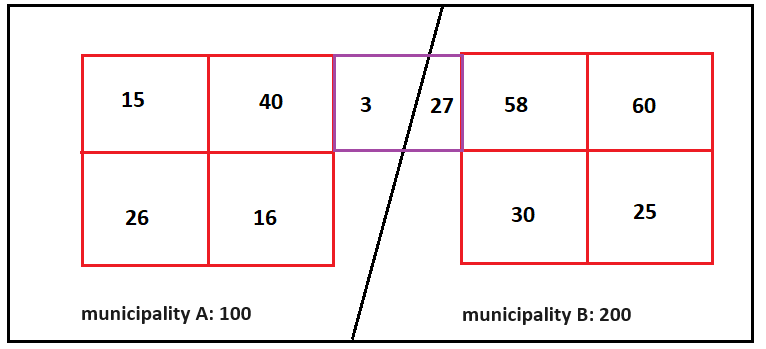
\includegraphics[width=\linewidth]{figures/Differencing_issues/protection_process_0_en.png}
\caption{A first example of geographical differencing.}
\label{fig:cas_complex_12}
\end{figure}

Figure~\ref{fig:cas_complex_12} represents two municipalities and all the  $1$~km $\times$ $1$~km grid tiles intersecting at least one of the municipalities. Municipality $A$ has $100$~households, municipality $B$ has $200$. The number of households in each of the tiles is also disseminated. Let us consider that an information is considered confidential if it concerns fewer than $4$ households. Releasing household counts over both geographical areas generates no direct confidentiality issue, all counts being greater than $4$.

As two sets are released, the difference can be processed:

\begin{equation}
    \begin{split}
    A &= 100 = 15 + 40 + 26 + 16 + A^{\cap B} \\
    B &= 200 = 58 + 60 + 30 + 25 + B^{\cap A} \\
    %30 &= x + y , no need for this equation
    \end{split}
    \label{eq:diff_interne}
\end{equation}

where:

\begin{itemize}
\item \(A^{\cap B}\) denotes the number of households in the tile intersecting A and B residing in municipality A.
\item \(B^{\cap A} \) denotes the number of households in that tile residing in municipality B. 
\end{itemize}

We then obtain the following indirectly released information :

\begin{equation}
    \begin{split}
    A^{\cap B} &= 3 \\
    B^{\cap A} &= 27 
    \end{split}
    \label{eq:diff_interne2}
\end{equation}

In this specific case, an attacker can easily retrieve a confidential information by differencing the two areas.


As \cite{Costemalle_2019} introduced a systematic detection of differencing issues, the following subsections will be based on the way the problem is described there.

\subsection{Internal and external differencings}

The \textit{internal region} of the municipality $A$ is composed by all the tiles which are fully included in $A$ \citep{Costemalle_2019}. If $A_{intern}$ and $B_{intern}$ denote the counts associated with internal regions of $A$ and $B$ respectively, we get from the figure~\ref{fig:cas_complex_12}:

\begin{equation}
    \begin{split}
    A_{intern} &= 15+40+26+16 = 97 \\
    B_{intern} &= 58+60+30+25 = 173 
    \end{split}
    \label{eq:internal_regions}
\end{equation}

An \textit{internal differencing} is then the difference between an area and its internal region, as shown in equation~(\ref{eq:diff_internal}) for $A$ and $B$ municipalities.

\begin{equation}
    \begin{split}
    A - A_{intern} &= 100 - 97 = 3 \\
    B - B_{intern} &= 200 - 173 = 27 
    \end{split}
    \label{eq:diff_internal}
\end{equation}

Symmetrically, the \textit{external region} of the municipality $A$ is composed by all the tiles which are fully included \emph{or} partially included in $A$ \citep{Costemalle_2019}. If $A_{extern}$ and $B_{extern}$ denote the external regions of $A$ and $B$ respectively, we get from the figure~\ref{fig:cas_complex_12}:

\begin{equation}
    \begin{split}
    A_{extern} &= 15+40+26+16+30 = 127 \\
    B_{extern} &= 58+60+30+25+30 = 203 
    \end{split}
    \label{eq:external_regions}
\end{equation}

An \textit{external differencing} is then the difference between an area and its external region, as shown in the equation~(\ref{eq:diff_external}) for $A$ and $B$ municipalities.

\begin{equation}
    \begin{split}
    A_{extern} - A &= 127 - 100 = 27 \\
    B_{extern} - B &= 203 - 200 = 3 
    \end{split}
    \label{eq:diff_external}
\end{equation}

Hence, a differencing issue, for a given region $A$, occurs when the internal or external difference is under the threshold but greater than $0$.

\subsection{Complexity}

\begin{figure}[H]
    \centering
    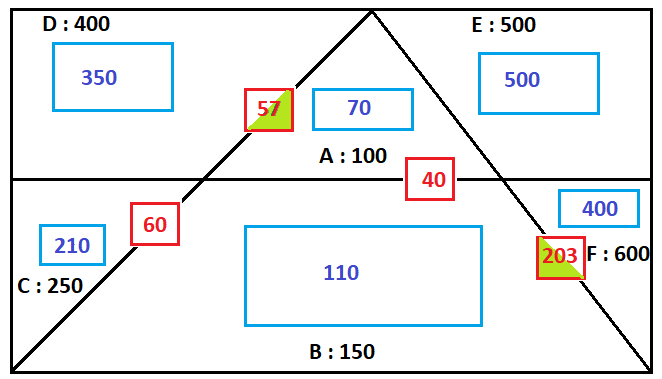
\includegraphics[width=0.8\linewidth]{figures/Differencing_issues/schema_intermediaire.png}
    \caption{A more complex differencing case.}
    \vspace{0.1cm}
    \raggedright \textit{Reading Note: In black the population of municipalities; in blue the number of households in tiles internal to municipalities; in red the number of households in tiles intersecting 2 municipalities.}
    \label{fig:schema_inter}
\end{figure}

Figure~\ref{fig:schema_inter} shows a case that is a little bit more complex, with six municipalities ($A, \dots , F$) whose household counts are displayed in black. The internal counts of each municipality are represented by the blue squares and the overlapping tiles by the red squares. 

Internal and external differencing can be performed for each municipality. For example, applying external differencing to the municipality $F$, we get $F_{extern} - F = 603 - 600 = 3$, which discloses a confidential information according to the chosen threshold. This external differencing is the counterpart of the internal differencing of the area composed by $A$, $B$, $C$ and $D$: $ABCD - ABCD_{intern} = 100 + 150 + 250 + 400) - (70 + 40 + 110 + 60 + 210 + 350 + 57) = 900 - 897 = 3$. Hence, possibly involving many areas at once, differencing problems can be hard to detect with real geographical areas.


\subsection{Method to detect differencing problems implemented in the \texttt{diffman} package} \label{sec:risk_diff_diffman}

When releasing data over administrative areas and $1$~km grid cells at a country scale,
the number of combinations to monitor for differencing issues is too large to be done in a reasonable time.\footnote{
    The method developed by \cite{Costemalle_2019} can be applied on any geographical areas. Here, we take a realistic example for an NSI: the superposition of an administrative partition of a country with a grid partition. In France, the municipality partition is composed of $35$~$000$ areas and the grid partition of $150$~$000$ square cells.}
\cite{Costemalle_2019} introduces a graph representation of the data and a way to explore and reduce it efficiently to detect differencing issues. This method is implemented in the R package \texttt{diffman} \citep{diffman}.

\begin{figure}[H]
\centering
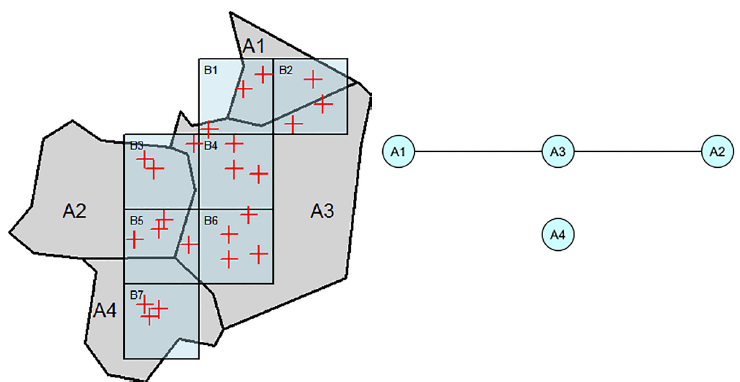
\includegraphics[width=0.9\linewidth]{figures/Differencing_issues/to_graph.png}
\caption{Overlapping areas and the corresponding graph; source: \citet{Costemalle_2019}.}
%\vspace{0.15 cm}
\raggedright \textit{\footnotesize Reading note: The graph on the right shows the links between the municipalities. The municipality $A1$ is linked to $A3$ because the tile $B1$ crosses both municipalities and has a population in each of them ($2$ in $A1$ and $1$ in $A3$).}
\label{fig:graph_ex}
\end{figure}

First, a graph is built by linking areas: two areas are connected, if a tile has its population spread across both of them. Figure~\ref{fig:graph_ex} shows an overlapping case and its corresponding graph. Area $A4$ is not connected to the others, since no tile is populated at once in $A4$ and another area. This first step builds some independent connected sub-graphs that can be handled separately.

As the first step can generate very large sub-graphs, \cite{Costemalle_2019} introduces several ways of reducing each of them, including merging nodes (zones) if the population of tiles that connect them is above the threshold in each zone (see Fig.~\ref{fig:merge_nodes}). Next, each sub-graph is split in smaller components according to the complementarity of internal and external differences. Finally, these differences are applied to all the sub-graphs to detect differencing issues (i.e. overlapped areas with population below a given threshold).


\begin{figure}[H]
\centering
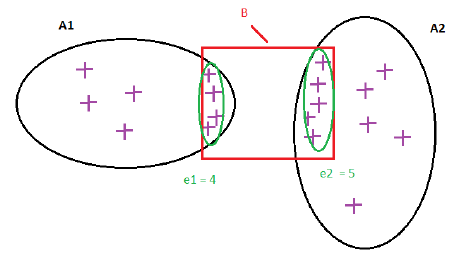
\includegraphics[width=0.7\linewidth]{figures/Differencing_issues/merge_nodes.png}
\caption{Merging nodes}
\vspace{0.15 cm}
\textit{\footnotesize Reading note: As the connecting tile has a population above the threshold in $A1$ ($e1=4$) and in $A2$ ($e2=5$), the two areas will be merged together in the graph.}
\label{fig:merge_nodes}
\end{figure}

In practice, the user of the package \texttt{diffman} \citep{diffman} only needs to call the \texttt{find\_pbm\_diff()} function to detect the differencing issues between two sets of non-nested areas.

\subsection{How to prevent geographical differencing issues}

Once detected, how can differencing problems be prevented? 

\cite{BuronFontaine2018} list four possibilities:

\begin{itemize}
    \item If areas can be modified, redraw their borders so as to eliminate the overlaps;
    \item if areas can't be redrawn, merge some of them so as to eliminate the overlaps;
    \item suppress some data;
    \item perturb some data.
\end{itemize}

\subsubsection{Suppressive approach}

With a suppressive method (see section \ref{sec:aux_suppr}), the suppression of the overlapping zone is inefficient. Actually, to prevent both internal and external differencing, one has to suppress one tile in the internal region and one tile in the external region.

In Figure~\ref{fig:prevent}, in order to avoid differencing the two tiles in blue have to be suppressed. The left one prevents the internal differencing and the right one prevents the external differencing.

\begin{figure}[ht]
\centering
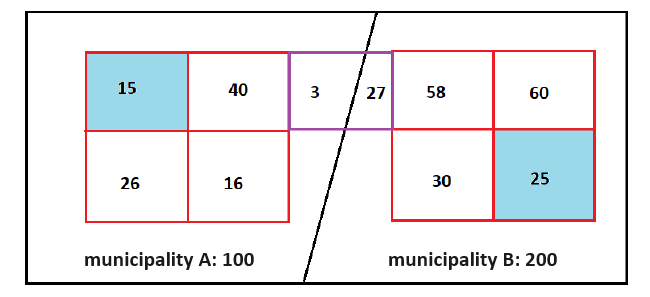
\includegraphics[width=0.8\linewidth]{figures/Differencing_issues/prevent_2_en.png}
\caption{Suppression pattern against differencing.}
\vspace{0.15 cm}
\textit{\footnotesize Reading note: The blue tiles are the suppressed tiles, preventing differencing.}
\label{fig:prevent}
\end{figure}

It is quite difficult to prevent geographical differencing issues with a suppressive approach in some real cases, such as census releases. Indeed, if many geographical sets of areas are released at the same time, the differencing potential has to be checked for every combination of overlapping sets. Nevertheless, if nested areas are used, it is sufficient to check and fix differencing issues with the smallest areas and the overlapping ones.

\subsubsection{Perturbative approach}

A perturbative approach can tackle the problem efficiently and systematically if and only if the method injects noise in \emph{every} cell, like the Cell Key Method (section \ref{sec:ckm}) or any rounding or noise injection method. A swapping method (section \ref{sec:trs}), for example, doesn't tackle the problem on its own.


\chapter{Information Loss Measures for Geo-Referenced Data} \label{sec:util}
\chaptermark{Information Loss Measures}

When an SDC method is applied to reduce the risks shown in Chapter \ref{sec:risk}, invariably some spatial aggregates may need to be altered, coarsened, or otherwise changed, leading to a loss of information compared to unprotected data. This chapter discusses how to assess such information loss, while keeping in mind the specific spatial character of the data.

\section{Measures of distributional distance} \label{sec:util_DD}

A grid map of frequency counts can be interpreted as a two-dimensional frequency distribution, visualised as a spatial histogram. Distortion of such a distribution can be measured by distance metrics between the original, unprotected map and the protected map.

\subsection{Hellinger Distance, Mean Squared Error, Mean Absolute Error} \label{sec:util_DD_hd}

The Hellinger Distance (HD) is an information-theoretical distance measure between two distributions. Its use in assessing the information loss after tabular data protection is well established, see e.g. \cite{ShlomoEtAl2015}, \cite{AntalEtAl2017}, \cite{ShlomoYoung2006} as well as \citet[4.7.2]{HundepoolEtAl2024}. An application to grid maps is described in \cite{GussenbauerEtAl2023}.

Formally, let us number the cells in the grid by $j = 1, \dots, M$. The original cell-level aggregates $X_j$ are compared to the aggregates after protection, which we call $X'_j$.
The Hellinger distance is defined as
\begin{equation} \label{eq:util_hd}
\mathrm{HD}\,(X, X') = \frac{1}{\sqrt{2}} \sqrt{\sum_{j=1}^M \left (\sqrt{X'_j} - \sqrt{X_j} \right )^2}.
\end{equation}

If $X_j$ and $X'_j$ are counts, the Hellinger distance is between 0 and $\sqrt{N}$, where $N$ is the sum of counts over the whole map \citep{ShlomoEtAl2015}.\footnote{
    This holds whenever the SDC mechanism does not change the total sum of counts $N$. For rounding-based or noise-based methods (like CKM; see section \ref{sec:ckm}) this may not be so. In that case the Hellinger distance is between 0 and the more general upper bound $\sqrt{N' + N} / \sqrt{2}$ (where $N'$ is the total sum of altered counts over the map).
} Alternatively, both $X$ and $X'$ can be re-scaled to the form of a discrete probability distribution, such that $X_j$ and $X'_j$ each sum to 1. In that case $\mathrm{HD} \in [0 \,, 1]$.
In any case a Hellinger distance of 0 signifies no information loss.

\subsubsection{Comparing HD and MSE / MAE}

The Hellinger distance may be contrasted with two other prevailing measures. The Mean squared error (MSE) and Mean absolute error (MAE) are common descriptive statistics that can be given a distance interpretation.
Formally, they are defined as follows:
\begin{equation} \label{eq:util_mse}
\mathrm{MSE}\,(X, X') = \frac{1}{M} \sum_{j=1}^M \left(X'_j - X_j\right)^2
\end{equation}
\begin{equation} \label{eq:util_mae}
\mathrm{MAE}\,(X, X') = \frac{1}{M} \sum_{j=1}^M \left| X'_j - X_j \right|.
\end{equation}

When choosing a measure for comparison, data suppliers should consider the following principle:
\textit{A distance measure between (spatial) distributions is useful, when an increase in distance is indicative of a deterioration of the perturbed map in comparison to the original.}\\

\begin{tcolorbox}[breakable]
\emph{Example}:
Consider the following simplified distribution of counts over a 4 $\times$ 4 grid map:
\[ 
\mathbf{X} = \begin{matrix} 
0 & 0 & 0 & 0 \\
0 & 4 & 1 & 0 \\
0 & 4 & 1 & 0 \\
0 & 0 & 0 & 0 \\
\end{matrix}
\]
We will compare this distribution with two ``perturbed" maps, labelled $\mathbf{X}'_{(1)}$ and $\mathbf{X}'_{(2)}$ respectively:
\[
\mathbf{X}'_{(1)} =
\begin{matrix} 
1 & 1 & 1 & 1 \\
1 & 0 & 0 & 1 \\
1 & 0 & 0 & 1 \\
1 & 0 & 0 & 1 \\
\end{matrix}\hspace{1cm}
\mathbf{X}'_{(2)} =
\begin{matrix} 
0 & 0  & 0 & 0 \\
0 & 0  & 0 & 0 \\
0 & 10 & 0 & 0 \\
0 & 0  & 0 & 0 \\
\end{matrix} 
\]
Results for MSE, MAE and HD are shown in Table \ref{tab:util_hd_mae_mse}.
The Hellinger distance has the property that it reaches its theoretical maximum when the underlying distributions have \textit{disjoint spatial support}. Practically speaking, this means that all previously inhabited areas would be uninhabited, arguably a \emph{worst case} for mapping. This is shown in $\mathbf{X}'_{(1)}$.

On the other hand, $\mathbf{X}'_{(2)}$ exemplifies an aggregation of the populated part of $\mathbf{X}$ (symbolizing a town, village or similar) to a smaller sub-area within. While this may be a grave error, it is arguably less so than the one shown in $\mathbf{X}'_{(1)}$. 
Looking at Table \ref{tab:util_hd_mae_mse}, we find that comparing the original $\mathbf{X}$ to $\mathbf{X}'_{(1)}$ yields the maximum Hellinger distance. The MSE, however, is lower when comparing $\mathbf{X}$ to $\mathbf{X}'_{(1)}$ than when comparing to $\mathbf{X}'_{(2)}$. The Hellinger distance is here more in line with the assumed rationale of the map maker.\footnote{
    It is granted that such extreme deviations as $\mathbf{X}'_{(1)}$ are unlikely to occur in practice. Nevertheless, populating at least some unpopulated cells is a common feature of several spatial SDC mechanisms, and it is good practice to consider what kind of data distortion would constitute a worst case.}\\

Another property of the Hellinger distance is of interest when comparing spatial distributions. To display it, consider two more perturbations of $\mathbf{X}$, labelled $\mathbf{X}'_{(3)}$ and $\mathbf{X}'_{(4)}$ shown below. Both maps differ from $\mathbf{X}$ by having one tenth of the distribution mass shifted between neighboring grid cells.
\[
\mathbf{X}'_{(3)} =
\begin{matrix} 
0 & 0 & 0 & 0 \\
0 & 5 & 1 & 0 \\
0 & 3 & 1 & 0 \\
0 & 0 & 0 & 0 \\
\end{matrix} \hspace{1cm}
\mathbf{X}'_{(4)} =
\begin{matrix} 
0 & 0 & 0 & 0 \\
0 & 4 & 2 & 0 \\
0 & 4 & 0 & 0 \\
0 & 0 & 0 & 0 \\
\end{matrix}
\]
Again, distance measures are shown in Table \ref{tab:util_hd_mae_mse}. It can be seen that MSE and MAE do not distinguish between $\mathbf{X}'_{(3)}$ and $\mathbf{X}'_{(4)}$. For mapping purposes however, shifting mass between two high-population areas $(\mathbf{X}'_{(3)})$ may be seen as a smaller error than doubling the population in one area and depopulating another $(\mathbf{X}'_{(4)})$. This rationale is covered by the Hellinger distance, but not by MSE and MAE.\footnote{
    This is because HD sums squared deviations of square roots, which penalizes large \emph{relative} changes \citep{AntalEtAl2017}, while MSE and MAE depend on \emph{absolute} changes.}

\begin{table}[H]
    \centering
    \begin{tabular}{c | c c c | c c c |}
            \multirow{2}{*}{$\mathbf{X}$ vs. }& \multicolumn{3}{c}{count} & \multicolumn{3}{c}{scaled} \\
               & MSE & MAE & HD & MSE & MAE & HD \\
        \hline
    $\mathbf{X}'_{(1)}$ & 2.75 & 1.25 & 3.16 & 0.028 & 0.125 & 1.000 \\
    $\mathbf{X}'_{(2)}$ & 3.38 & 0.75 & 1.92 & 0.033 & 0.075 & 0.606 \\
    $\mathbf{X}'_{(3)}$ & 0.13 & 0.13 & 0.25 & 0.001 & 0.013 & 0.080 \\
    $\mathbf{X}'_{(4)}$ & 0.13 & 0.13 & 0.77 & 0.001 & 0.013 & 0.242 \\
        \hline
    \end{tabular}
    \caption{Distributional distances between maps $\mathbf{X}$ vs. $\mathbf{X}'_{(1)}, \dots, \mathbf{X}'_{(4)}$}
    \label{tab:util_hd_mae_mse}
\end{table}
\end{tcolorbox}


\subsection{Earth Mover distance / Wasserstein distance} \label{sec:util_DD_kwd}

The Earth Mover distance, also known as \emph{Kantorovich-Wasserstein distance} (KWD), or simply Wasserstein distance, is a distance measure between distributions applicable to spatial histograms. While it is more demanding to compute than the metrics from \ref{sec:util_DD_hd}, it offers some theoretical advantages. 
We begin by showing a limitation of the HD, MSE, and MAE metrics introduced above.

\begin{tcolorbox}[breakable]
\emph{Example}:
Consider the following case of a (very much simplified) count distribution in a 4 $\times$ 4 grid map. The example is adapted from \cite{GussenbauerEtAl2023} and \cite{RicciatoGualandi2024}. 10 population units are spread over 5 grid cells, symbolizing a small spatial cluster:
\[
\mathbf{X} = \begin{matrix} 0 & 2 & 0 & 0 \\
                  2 & 2 & 2 & 0 \\
                  0 & 2 & 0 & 0 \\
                  0 & 0 & 0 & 0 \end{matrix}
\]
We now offer four hypothetical perturbations, shown as $\mathbf{X}'_{(1)}, \dots, \mathbf{X}'_{(4)}$ below. Loosely, the first two $(\mathbf{X}'_{(1)} \text{ and } \mathbf{X}'_{(2)})$ correspond to shifting some units around in space, whereas the latter two $(\mathbf{X}'_{(3)} \text{ and } \mathbf{X}'_{(4)})$ are different local aggregations.
\begin{align*}
\mathbf{X}'_{(1)} = \begin{matrix} 0 & 0  & 2 & 0 \\
                          2 & 2  & 2 & 0 \\
                          2 & 0  & 0 & 0 \\
                          0 & 0  & 0 & 0 \end{matrix} & \hspace{1cm}
\mathbf{X}'_{(2)} = \begin{matrix} 0 & 0  & 0 & 2 \\
                          2 & 2  & 2 & 0 \\
                          0 & 0  & 0 & 0 \\
                          0 & 0  & 0 & 2 \end{matrix} \\ & \\
\mathbf{X}'_{(3)} = \begin{matrix} 0 & 0  & 0  & 0 \\
                          0 & 10 & 0  & 0 \\
                          0 & 0  & 0  & 0 \\
                          0 & 0  & 0  & 0 \end{matrix} & \hspace{1cm}
\mathbf{X}'_{(4)} = \begin{matrix} 0 & 0  & 0  & 0 \\
                          0 & 0  & 10 & 0 \\
                          0 & 0  & 0  & 0 \\
                          0 & 0  & 0  & 0 \end{matrix}
\end{align*}
Most data suppliers would judge $\mathbf{X}'_{(2)}$ inferior to $\mathbf{X}'_{(1)}$, since the former shifts units \emph{further away} than the latter, compared to the true distribution $\mathbf{X}$. Similarly, in $\mathbf{X}'_{(3)}$ and $\mathbf{X}'_{(4)}$, while the information loss from aggregation is the same, the latter also shifts the \emph{geometrical center} of the distribution, while the former keeps it.
It would thus be reasonable to demand a distance measure which gives us $\mathrm{Dist.}(\mathbf{X}, \mathbf{X}'_{(2)}) > \mathrm{Dist.}(\mathbf{X}, \mathbf{X}'_{(1)})$ and $\mathrm{Dist.}(\mathbf{X}, \mathbf{X}'_{(4)}) > \mathrm{Dist.}(\mathbf{X}, \mathbf{X}'_{(3)})$.\footnote{
    Recall our principle stated above: \textit{a distance measure is useful insofar as an inferior map is associated with a larger distance}.}
    
Actual distributional distances are given in Table \ref{tab:util_nokwd}. 
For any given measure introduced so far we get $\mathrm{Dist.}(\mathbf{X}, \mathbf{X}'_{(2)}) = \mathrm{Dist.}(\mathbf{X}, \mathbf{X}'_{(1)})$ and $\mathrm{Dist.}(\mathbf{X}, \mathbf{X}'_{(4)}) = \mathrm{Dist.}(\mathbf{X}, \mathbf{X}'_{(3)})$. In other words, these metrics are not discriminating quite as we would want them to.\footnote{
    The reason is that changes in mere \emph{position} are not taken into account.}

\begin{table}[H]
    \centering
    \begin{tabular}{c | c c c |}
    $\mathbf{X}$ vs. & MSE & MAE & HD \\
    \hline
    $\mathbf{X}'_{(1)}$ & 1.00 & 0.50 & 2.00 \\
    $\mathbf{X}'_{(2)}$ & 1.00 & 0.50 & 2.00 \\
    \hline
    $\mathbf{X}'_{(3)}$ & 5.00 & 1.00 & 2.35 \\
    $\mathbf{X}'_{(4)}$ & 5.00 & 1.00 & 2.35 \\
        \hline
    \end{tabular}
    \caption{MSE, MAE, and HD between maps $\mathbf{X}$ vs. $\mathbf{X}'_{(1)}, \dots, \mathbf{X}'_{(4)}$}
    \label{tab:util_nokwd}
\end{table}
\end{tcolorbox}

Generally speaking, such concepts as `further away' and `shifted geometrical center' are not covered by the distributional distances of section \ref{sec:util_DD_hd}. They do not explicitly take the \emph{spatial dimension of error} into account. The Kantorovich-Wasserstein distance (KWD), on the other hand, does this, by conceptualizing the distance between distributions as a problem of \emph{optimal transport}.
The idea is to transform one distribution, say the perturbed $X'$, into the other, say the original $X$, by transporting units (or, more generally: distribution mass) around the map, until both distributions look alike. Each act of transportation is evaluated at `costs' equivalent to the geographical distance covered.
%\footnote{
    %Shifting 2 units by 3 cells to the left 'costs' $2 \cdot 3 = 6$, etc. We consider here for the geographical distance the Euclidean, or straight-line distance, but KWD generalizes to others, such as the Manhattan distance. Units that do not need to be moved are evaluated at zero 'costs'.}
KWD is defined as the total cost of the `cheapest' way to perform such a transformation.

Formally, computing KWD involves solving the following optimization problem. We denote the shifted distribution mass (e.g. a certain number of population units) between grid cell $j$ and $k$ by $\Delta X_{jk}$. The (spatial) distance between these grid cells is $d_{jk}$. We then need to solve:
\begin{equation} \label{eq:util_kwd}
\begin{aligned}
    & \mathrm{KWD}\,(X, X') = & \underset{\Delta X_{jk}}{\text{min}} \quad & \frac{1}{N} \sum_{j=1}^M \sum_{k=1}^M \Delta X_{jk} \cdot d_{jk} & \\
    & & \text{s.t.} \quad & \sum_{k=1}^M \Delta X_{jk} = X_j & \forall j = 1, \dots, M\\
    & & & \sum_{j=1}^M \Delta X_{jk} = X'_k & \forall k = 1, \dots, M \\
    & & & \Delta X_{jk} \geq 0 & \forall j,k = 1, \dots, M.
\end{aligned}
\end{equation}

\begin{tcolorbox}[breakable]
\emph{Example cont'd:}
Going back to our example, we find that transforming $\mathbf{X}'_{(1)}$ back to $\mathbf{X}$ is most efficiently achieved by conceptually shifting the 2 units in the first row one cell to the left, the 2 units in the third row one cell to the right. This is associated with a combined `cost' of $2 \cdot 1 + 2 \cdot 1 = 4$, hence $\mathrm{KWD}(\mathbf{X}, \mathbf{X}'_{(1)}) = 4/10 = 0.4$. The optimal transport plan for $\mathbf{X}'_{(2)}$ gives us $2 \cdot 2 + 2 \cdot \sqrt{1^2 + 2^2} \approx 8.47$, therefore $\mathrm{KWD}(\mathbf{X}, \mathbf{X}'_{(2)}) \approx 0.85$.\footnote{
    By analogous reasoning we can find out that $\mathrm{KWD}(\mathbf{X}, \mathbf{X}'_{(4)}) > \mathrm{KWD}(\mathbf{X}, \mathbf{X}'_{(3)})$.}
In other words, the KWD discriminates in line with the assumed judgment of the data supplier, where (in this case) MSE, MAE, and HD did not.
\end{tcolorbox}

\subsubsection{Practical issues}

Computing KWD in practice requires a solver for the optimization procedure, as problems are not as simple as in the motivating example. When the number of bins in the spatial histogram is large, an exact solution may not be feasible computationally. \cite{BassettiEtAl2020} provide a method to approximate KWD in these cases. A ready-to-use implementation for the R software is the \texttt{SpatialKWD} package.
An example use for comparing spatial histograms by KWD is given in \cite{RicciatoColuccia2023}. An application specifically for assessing the impact of SDC is \cite{GussenbauerEtAl2023}.


\section{Measures of spatial association} \label{sec:util_SPAT}

\subsection{Variance-Mean ratio}

The Variance-Mean ratio (VMR) is a measure of dispersion. It can be used as a descriptive statistic to measure the overall level of spatial clustering in geo-referenced data \citep{Cressie1993}. Intuitively, if the distribution of population over a map is relatively homogeneous, then cell counts everywhere will not differ much from the average cell count. If, on the other hand, population is concentrated at one or a few points of the map and thin between, a high variance of counts results. By comparing the VMR before and after disclosure control, a first indication is given as to how the level of clustering is impacted.\footnote{
    Note: If the total number of population units in the map is not changed by SDC, then the mean too will stay the same and comparing VMR reduces to comparing the variance of the count distribution.} 

Formally, the VMR is measured as
\begin{equation}
    \mathrm{VMR}\,(X) = \frac{\frac{1}{M}\sum_{j = 1}^M (X_j - \bar{X})^2}{\bar{X}} = \frac{\mathrm{Var}(X)}{\mathrm{Mean}(X)}.
\end{equation}

The difference $\mathrm{VMR}\,(X') - \mathrm{VMR}\,(X)$ is positive if SDC has increased the level of spatial clustering, negative if it has decreased it.\\

If there exist only very few outliers and their impact on total dispersion is expected to be reduced then instead of $\mathrm{VMR}$ one can use its positional counterpart, i.e. MedAD-Median ratio, given as:

\begin{equation}
    \mathrm{MMR}\,(X) = \frac{\mathrm{MedAD}(X)}{\mathrm{Med}(X)},
\label{MMR}
\end{equation}
where $\mathrm{MedAD}(X)=\mathrm{Med}_{j=1,2,\ldots,M}|X_j-\mathrm{Med}(X)|$ is the Median Absolute Deviation of $X$. The interpretation of the difference $\mathrm{MMR}\,(X') - \mathrm{MMR}\,(X)$ is the same as $\mathrm{VMR}\,(X') - \mathrm{VMR}\,(X)$. The main limitation of (\ref{MMR}) is that when most cell counts are zero (in sparse grid data, for instance), it cannot be computed. Hence, MMR is useful only for such grids, where all (or almost all) data are non-zero.

On the other hand, one could be afraid that the double-use of the median (median absolute deviation from the median) in (\ref{MMR}) is somewhat `too robust'. That is, one can get the same MMR, even though the map has changed, which would not be informative.
To reduce the latter inconvenience, one can suggest also two alternative approaches. Firstly, the MedADM-Med ratio:
\begin{equation}
    \mathrm{MMR^*}\,(X) = \frac{\mathrm{MedADM}(X)}{\mathrm{Med}(X)},
\label{MMRx}
\end{equation}
where $\mathrm{MedADM}(X)=\mathrm{Med}_{j=1,2,\ldots,M}|X_j-\bar{X}|$ is the median absolute deviation from the mean. Secondly, the MeanAD-Med ratio:
\begin{equation}
    \mathrm{MMR^{**}}\,(X) = \frac{\mathrm{MeanAD}(X)}{\mathrm{Med}(X)},
\label{MMRxx}
\end{equation}
where 
%$\mathrm{MeanAD}(X)=\frac{\sum_{j=1}^M{|X_j-\mathrm{Med}(X)|}}{M}$. 
$\mathrm{MeanAD}(X)= \frac{1}{M} \sum_{j=1}^M |X_j-\mathrm{Med}(X)|$ is the mean absolute deviation from the median.
However, the problematic case of $\mathrm{Med}(X) = 0$ still exists both in (\ref{MMRx}) and in (\ref{MMRxx}). One can try to overcome it by assuming instead of a ``pure" median in (\ref{MMR}), (\ref{MMRx}) and (\ref{MMRxx}) the corrected median defined as follows:
\begin{equation}
\mathrm{\widetilde{med}}(X)=\mathrm{med}(X)+\frac{\mathop{\min}\limits_{j:X_{j}\ne 0}{|X_{j}|}}{M}.
\label{MEDc}
\end{equation}

\begin{tcolorbox}[breakable]
\emph{Example}:
$\mathbf{X}$ below shows a $6 \times 6$ grid map with original counts. $\mathbf{X}'$, to its right, shows a protected version. We want to calculate VMR and MMR.
\[ 
\mathbf{X} = \begin{matrix} 
2 & 4 & 0 & 0 & 0 & 0\\
4 & 2 & 0 & 0 & 0 & 0\\
0 & 0 & 2 & 3 & 2 & 0\\
0 & 0 & 0 & 5 & 4 & 1\\
0 & 0 & 3 & 4 & 2 & 0\\
0 & 0 & 0 & 4 & 0 & 2\\
\end{matrix}
\hspace{1cm}
\mathbf{X}' = \begin{matrix} 
3 & 3 & 0 & 0 & 0 & 0\\
3 & 3 & 0 & 0 & 0 & 0\\
0 & 0 & 2 & 2 & 2 & 2\\
0 & 0 & 2 & 2 & 2 & 2\\
0 & 0 & 2 & 2 & 2 & 2\\
0 & 0 & 2 & 2 & 2 & 2\\
\end{matrix}
\]
The sum of counts is 44 in both maps; hence the mean is $44/36 \approx 1.22$. For the variance we get 2.69 (left) and 1.32 (right) respectively. This gives us for the change in VMR:
\[
\mathrm{VMR}(\mathbf{X}') - \mathrm{VMR}(\mathbf{X})
= \frac{1.32}{1.22} - \frac{2.69}{1.22} \approx - 1.12.
\]
Because $\mathrm{med}(\mathbf{X})=0$, we cannot use directly measures (\ref{MMR}), (\ref{MMRx}) and (\ref{MMRxx}). However, we can use (\ref{MEDc}) and obtain $\mathrm{\widetilde{med}}(\mathbf{X})=0,028$ and $\mathrm{\widetilde{med}}(\mathbf{X}')=2,056$. Hence, $\mathrm{MedAD}(\mathbf{X}')=0.944$, $\mathrm{MedAD}(\mathbf{X})=0.028$, $\mathrm{MedADM}(\mathbf{X}')=1.222$, $\mathrm{MedADM}(\mathbf{X})=1.222$, $\mathrm{MeanAD}(\mathbf{X}')=1.043$, $\mathrm{MeanAD}(\mathbf{X})=1.227$ and in consequence,   the corrected measures are as follows 
\[
\mathrm{MMR}(\mathbf{X}') - \mathrm{MMR}(\mathbf{X})
= \frac{0.944}{2.056} - \frac{0.028}{0.028} \approx -0.541,
\]
\[
\mathrm{MMR^*}(\mathbf{X}') - \mathrm{MMR^*}(\mathbf{X})
= \frac{1.222}{2.056} - \frac{1.222}{0.028}\approx -43.405,
\]
and
\[
\mathrm{MMR^{**}}(\mathbf{X}') - \mathrm{MMR^{**}}(\mathbf{X})
= \frac{1.043}{2.056} - \frac{1.227}{0.028}\approx -43.659.
\]

This means the protected map has a markedly lower level of clustering compared to the original. However, the two last measures seem to slightly overestimate the information loss. 
\end{tcolorbox}


\subsection{Moran's $\mathcal{I}$} \label{sec:util_moran}

% Moran plots as a graphical/visual way to compare original and perturbed autocorrelations ? What do you think ?
% I make a proposition a the end of the subsection

The \emph{Moran's $\mathcal{I}$ statistic}, proposed by \cite{Moran1950}, was conceived as a measure of spatial autocorrelation of spatial objects. In general, the global Moran's $\mathcal{I}$ statistic is of the form
\begin{equation}
    \mathcal{I}\stackrel{df}{=}\frac{n}{w}\frac{\sum_{i=1}^n{\sum_{j=1}^n{w_{ij}(x_i-\overline{x})(x_j-\overline{x})}}}{\sum_{i=1}^n{(x_i-\overline{x})^2}},
\label{globalI}
\end{equation}
where $n$ is the number of spatial units, $x_i$ is the value of the variable $X$ for $i$-th spatial unit, $\overline{x}$ is the mean of $X$ and $w_{ij}$ is the (non-negative) measure of closeness of $i$-th and $j$-th units with $w_{ii}=0$, ($i,j=1,2,\ldots,n$), $w=\sum_{i=1}^n{\sum_{j=1}^n{w_{ij}}}$.

Values of $\mathcal{I}$ belong usually to the interval $[-1,1]$.\footnote{If the matrix $\mathbf{W}=[w_{ij}],i,j=1,2,\ldots,n$ is symmetric and row--normalized.} Values significantly below $-1/(n-1)$ indicate negative spatial autocorrelation and values significantly above $-1/(n-1)$ indicate positive spatial autocorrelation. If $\mathcal{I}=-1$ then autocorrelation (dispersion) is perfect, if $\mathcal{I}=0$ then no autocorrelation occurs (i.e. we are dealing with perfect randomness). $\mathcal{I}=1$ indicates also perfect autocorrelation, but in the opposite direction.

In constructing (\ref{globalI}) the most important role seems to be played by the matrix of weights $\mathbf{W}=[w_{ij}]$, $i,j=1,2,\ldots,n$. It reflects the closeness of spatial units which can be defined in various ways. A classical approach in this context is based on physical neighbourhood, i.e. on existing common boundaries arbitrarily established (contiguity). More formally, two areas (e.g. grid tiles) are neighbours if they have a common frontier. Two approach in this respect are common: rook contiguity (when only common edges of polygons reflecting borders of given areas are considered to define the neighbor relation) or queen contiguity (when not only common edges but also common vertices are taken into account in this context). Due to better usefulness (e.g. for irregular polygons and reduction of possible inaccuracies) the use of queen criterion is recommended in practice. 

Alternatively, the neighbourhood can also be defined on the basis of a similarity of spatial units with regards to the distribution of a given composite social or economic phenomenon. The distance between given objects is here expressed by distance of vectors of values of relevant variables for them. Of course, they can include also some geographical information (e.g. country of birth), but it is not an absolute priority in this case. That is, it is assumed that such phenomenon is described by a number (say, $m$) variables. Each object is therefore described by a vector from $\mathbb{R}^m$. Using a relevant metric (e.g. Euclidean, city -- called also Manhattan, Minkowski, etc.) one can measure the distance between each pair of objects. The entries of matrix $\mathbf{W}$ can be simply such distances. Alternatively, $\mathbf{W}$ may be established in a binary way, i.e. as $w_{ij}=1$ (not neighbours) if $d_{ij}>q$ and $w_{ij}=0$ (neighbours) otherwise, where $d_{ij}$ is the distance between $i$-th and $j$-th objects and $q>0$ -- an arbitrarily established threshold. A more formal presentation and discussion on these topics was conducted by \cite{Mlodak2013}. The measures of information loss proposed in this paper were implemented to the \texttt{sdcMicro} R-package.   

It is worth noting that the variables describing the phenomenon being a base for identification of neighbourhood should be different than variables being perturbed in the SDC process (the neighbourhood is independent of the purpose of current analysis and cannot be perturbed). This means that only non-identifiers, non-quasi identifiers or non-sensitive variables can be used here.\\
%We could mention here the attention needed in choosing the matrix of weights (choosing contiguity or a distance, choosing a threshold beyond that the weights are set to zero, etc.) because it could have a substantial influence on the measure of the Moran I. Moreover, the matrix of weights has to be normalized, otherwise we create an heterogeinty between the units with a lot of neighbors and those with less. 
%(See \cite{BellefonEtAlt_2018})

An efficient measure of information loss due to global autocorrelation should satisfy the following expectations:
\begin{itemize}
    \item It should compare the loss of information of different SDC processes;
    \item it should be able to sort SDC processes in the right order w.r.t. distortion of spatial autocorrelation;
    \item it should clearly indicate the following situations, when they occur:
    \begin{itemize}
        \item a negative autocorrelation is weakened by the SDC process, 
        \item a positive autocorrelation is strengthened by the SDC process,
        \item a weak negative link is becoming a weak positive link by the SDC process;
    \end{itemize}
    \item it should provide information on the direction of the change (increase or decrease);
    \item it should be normalized on [-1,1].
\end{itemize}

It seems that these postulates are satisfied by the following measure:
\begin{equation}
\mathrm{ILM}\stackrel{df}{=}\frac{\mathcal{I}'-\mathcal{I}}{2},
\label{globalloss}
\end{equation}
where $\mathcal{I}'$ is the Moran's $\mathcal{I}$ global statistics (\ref{globalI}) after disclosure protection within the SDC process. The coefficient (\ref{globalloss}) takes value from $[-1,1]$ and hence can be presented in \%. If $\mathrm{ILM}=0$ then no loss is incurred, whereas $|\mathrm{ILM}|=1$ means the loss is maximal.%\\

\begin{tcolorbox}[breakable]
\emph{Example}:
Consider the following simplified distribution of counts over a 6 $\times$ 6 grid map, denoted by $\mathbf{X}$. Sensitive counts (considered here as any grid cell smaller than 5) are protected by two iterations of the quadtree mechanism (see section \ref{sec:quadtree}), yielding protected map $\mathbf{X}'$.

\[ 
\mathbf{X} = \begin{matrix} 
2 & 4 & 0 & 0 & 0 & 0\\
4 & 2 & 0 & 0 & 0 & 0\\
0 & 0 & 2 & 3 & 2 & 0\\
0 & 0 & 0 & 5 & 4 & 1\\
0 & 0 & 3 & 4 & 2 & 0\\
0 & 0 & 0 & 4 & 0 & 2\\
\end{matrix}
\hspace{1cm}
\mathbf{X}' = \begin{matrix} 
3 & 3 & 0 & 0 & 0 & 0\\
3 & 3 & 0 & 0 & 0 & 0\\
0 & 0 & 2 & 2 & 2 & 2\\
0 & 0 & 2 & 2 & 2 & 2\\
0 & 0 & 2 & 2 & 2 & 2\\
0 & 0 & 2 & 2 & 2 & 2\\
\end{matrix}
\]

We aim to measure Moran's $\mathcal{I}$, using as our criterion for neighbourhood the `queen'-contiguity (in other words, a grid cell is neighbour to the 8 cells surrounding it, including diagonally). With $6^2 = 36$ cells, the weight matrix $\mathbf{W}$ has 36 rows and 36 columns. The first row encodes all neighbors of the first cell ($i = 1$), of which there are three: directly east ($j = 2$), directly south ($j = 7$) and diagonally southeast ($j = 8$) -- most cells will have more neighbors, because they don't lie at a corner. For the first row of weights $w_{1j}$ we thus get
\[
w_{1j} = 1 \text{ for } j = 2,7,8 \text{ and } w_{1j} = 0 \text{ else}.
\]
To avoid the distorting effect of a differing number of neighbours between cells, we row-standardize to
\[
w_{1j} = \frac{1}{3} \text{ for } j = 2,7,8 \text{ and } w_{1j} = 0 \text{ else}
\]
so that $\sum_j w_{1j} = 1$. For all other rows we proceed likewise.\footnote{
    The creation of a weight matrix would be tedious if done by hand, hence this is usually accomplished by software. For instance, in the R-software, the package \texttt{spdep} can create weight matrices for arbitrarily shaped polygons and the package \texttt{raster} supplies an efficient implementation of weights for regular grids. Note that square grids have a particularly easy neighbourhood structure: all cells that do not lie at the map margin have exactly 8 (`queen'--)neighbours.}\\

Plugging into Eq. (3.6), the count distribution in grid map $\mathbf{X}$ yields a Moran's $\mathcal{I}$ of 0.288, while the quadtree results $\mathbf{X}'$ yield 0.502. Our suggested information loss measure gives then:
\[
\mathrm{ILM}=\frac{0.502-0.288}{2}=0.107
\]
The application of SDC leads here to an increase in Moran's $\mathcal{I}$. In magnitude this corresponds to an information loss with respect to spatial autocorrelation by 10.7\%.    

\end{tcolorbox}

Apart from the estimation of total information loss, assessment of the distribution of information loss on particular objects is often necessary. It can be based on the local Moran's $\mathcal{I}$ statistic discussed and developed by \cite{Anselin1995}. It is of the following form:
\begin{equation}
 \mathcal{I}_i\stackrel{df}{=}\frac{(n-1)(x_i-\overline{x})\sum_{j=1}^n{w_{ij}(x_j-\overline{x})}}{\sum_{j=1}^n{(x_j-\overline{x})^2}},
\label{localI}
\end{equation}
% In Anselin 1995, Local Moran is defined as follows:
%\begin{equation}
%  I_i\stackrel{df}{=}(x_i-\overline{x})\sum_{j=1}^n{w_{ij}(x_j-\overline{x})},
% \label{localI}
% \end{equation}
$i=1,2,\ldots,n$, where symbols used are the same as in (\ref{globalI}). The information loss can be here expressed by a comparison of basic characteristics of distributions of $\mathcal{I}_i$ and $\mathcal{I}'_i$ (where $\mathcal{I}_i$ denotes the original local Moran's $\mathcal{I}$ statistics and $\mathcal{I}'_i$ this quantity after perturbation of the data during the SDC process) for objects $i=1,2,\ldots,n$. It is worth remembering that the expected value of $\mathcal{I}_i$ is
\[
E(\mathcal{I}_i)=-\frac{\sum_{j=1}^n{w_{ij}}}{n-1},\quad i=1,2,\ldots,n.
\]

Alternatively, one can analyse in this context the distribution of absolute distances $d_i$ between both indices, i.e.
%\[
\begin{equation}
d_i\stackrel{df}{=}\left|\,\mathcal{I}'_i- \mathcal{I}_i\,\right|,\quad i=1,2,\ldots,n.
\label{eq:d_i}
\end{equation}
%\]

However, the formulas (\ref{globalI}) and (\ref{localI}) are based only on a single variable, whereas the data to be published cover often of a number of various variables. Therefore an assessment of a loss on the connections between them taking the spatial autocorrelation into account is also needed. For classical microdata some simple proposals and comparisons in this context were formulated e.g. by \cite{Domingo2001}. A more complex measure of information loss, but taking all (even hard to perceive) connections between continuous variables into account was suggested by \cite{Mlodak2022}. Their approach is based on the diagonal entries of the inverse correlation (usually Pearson's) matrix.

This solution can be used also in the currently discussed situation. Let $X$ and $Y$ be two variables for which correlation is to be assessed and consider the following modification of the global  Moran's $\mathcal{I}$ statistic
\begin{equation}
 \mathcal{I}_{XY}\stackrel{df}{=}\frac{n}{w}\frac{\sum_{i=1}^n{\sum_{j=1}^n{w_{ij}(x_i-\overline{x})(y_i-\overline{y})(x_j-\overline{x})(y_j-\overline{y})}}}{\sum_{i=1}^n{(x_i-\overline{x})^2(y_i-\overline{y})^2}}.
\label{globalIXY}
\end{equation}

Due to the properties of the classical global Moran's $\mathcal{I}$ statistics, the measure (\ref{globalIXY}) will also take values from $[0,1]$. If the investigated microdata set contains $m$ ($m\in\mathbb{N}$) continuous variables $X_1,X_2,\ldots,X_m$ then one can define a spatial correlation matrix $\mathbf{IC}\stackrel{df}{=}[\mathcal{I}_{X_kX_l}]$, $k,l=1,2,\ldots,m$. The diagonal entries of its inverse, $\mathbf{IC}^{-1}$, will be a basis for assessing information loss. That is, let $\mathbf{IC}$ be the Moran's correlation matrix for $X_1,X_2,\ldots,X_m$ in original data and $\mathbf{IC}'$ the relevant matrix for perturbed data. According to \cite{Mlodak2022}, the information loss can be then measured as
\begin{equation}
 \gamma_M\stackrel{df}{=}\frac{1}{\sqrt{2}}\sqrt{\sum_{j=1}^{m}{\left(\frac{\mathcal{I}_{jj}^{(-1)}}{\sqrt{\sum_{l=1}^m{\left(\mathcal{I}_{ll}^{(-1)}\right)^2}}}-\frac{\mathcal{I}_{jj}'^{\,(-1)}}{\sqrt{\sum_{l=1}^m{\left(\mathcal{I}_{ll}^{*(-1)}\right)^2}}}\right)^2}}\in [0,1],
\label{gammaM}
\end{equation}
where $\mathcal{I}_{ii}^{(-1)}$ and $\mathcal{I}_{ii}'^{\,(-1)}$ are diagonal entries of $\mathbf{IC}$ and $\mathbf{IC}'$, respectively. Of course, apart from the general case (\ref{gammaM}), one can also analyse the distances between the local spatial correlation of analysed variables for the $i$-th cell, using the formula
\begin{equation}
 {\gamma}M_i\stackrel{df}{=}\frac{(n-1)(x_i-\overline{x})(y_i-\overline{y})\sum_{j=1}^n{w_{ij}(x_j-\overline{x})(y_j-\overline{y})}}{\sum_{j=1}^n{(x_j-\overline{x})^2(y_j-\overline{y})^2}},
\label{lgammaM}
\end{equation}
$i=1,2,\ldots,n$. The distance between original (${\gamma}M_i$) and perturbed (${\gamma}M'_i$) local spatial correlation is then given as
%\[
\begin{equation}
dM_i\stackrel{df}{=}\left|{\gamma}M'_i-{\gamma}M_i\right|,\quad i=1,2,\ldots,n.
\label{eq:dM_i}
\end{equation}
%\]
The distribution of $dM$ over grid cells using (\ref{lgammaM}) is then a basis for assessment of information loss.  


\subsubsection{Using the Moran's diagram to visually assess the utility}

The Moran's diagram is a scatter plot, where each area (e.g. each grid tile) is represented by a point. Its coordinates are: on the x-axis the actual value taken by the variable, and on the y-axis the spatially lagged value, that is: the weighted mean of the neighbors of the area (as defined above). The variable is previously standardized and the weights are normalized (see \cite{BellefonEtAlt_2018} on the different ways to normalize the weights matrix), so that the origin of the axis represent the mean of the variable (0). 

Using the previous notations, $(\Tilde{x}_i\,, \sum_{j \neq i}{\Tilde{w}_{ij}\Tilde{x}_j})$ are the coordinates of an area $A_i$, where $\Tilde{x}_i$ is the value of $\Tilde{X}$, the normalized variable of $X$, for the $i$-th spatial unit. $\Tilde{w}_{ij}$ is the normalized weight of th $j$-th neighbor of $A_i$.

Hence, each of the four quadrants of the diagram corresponds to a specific spatial correlation between a unit and its neighbors. The north-east and the south-west quadrants correspond to a positive spatial autocorrelation, where the units resemble their neighbors, either sharing low values in the south-west (one can call it a low-low structure) or high values in the north-east quadrant (high-high structure). The north-west and the south-east quadrants correspond to a negative spatial autocorrelation, where the units are dissimilar to their neighbors, either in having a high value surrounded by low values in the south-east (a high-low structure) or a low value surrounded by high values in the north-west quadrant (low-high structure) (see \cite{SalimaEtAlt_2018} for more details on the Moran's diagram).

Based on this diagram, we can make a first assessment of how much the statistical disclosure control has disturbed the spatial relations. As an illustration of what could be the effect of a SDC method on the spatial associations, the figure~\ref{fig:moran_plot} compares three Moran's diagrams computed from the number of poor households in 569 tiles of 200m $\times$ 200m, somewhere in France:

\begin{itemize}
    \item The first one corresponds to the original data;
    \item In the second diagram (first row, second column), the data have been swapped, with a bandwidth of 400m;
    \item In the third one, the small cells (below 11) have been randomly rounded to 0 or 11.
\end{itemize}

The diagrams are comparable, because the neighborhood is based on the same \textit{queen} contiguity. We can notice that the clouds of points of the original and the rounded data have similar distribution. This is confirmed by relatively close Moran's $\mathcal{I}$. On the contrary, the smoothing reinforces the positive autocorrelation of the spatial distribution of poor households: the points cloud has a more elongated shape, along the regression line. This is confirmed by a much higher Moran's $\mathcal{I}$.

This first assessment can be confirmed by the computation of the $\mathrm{ILM}$ indicator (\ref{globalloss}): for the smoothing, we get $\mathrm{ILM} = 0.408$ and for the rounding method $0.0365$.

\begin{figure}
    \centering
    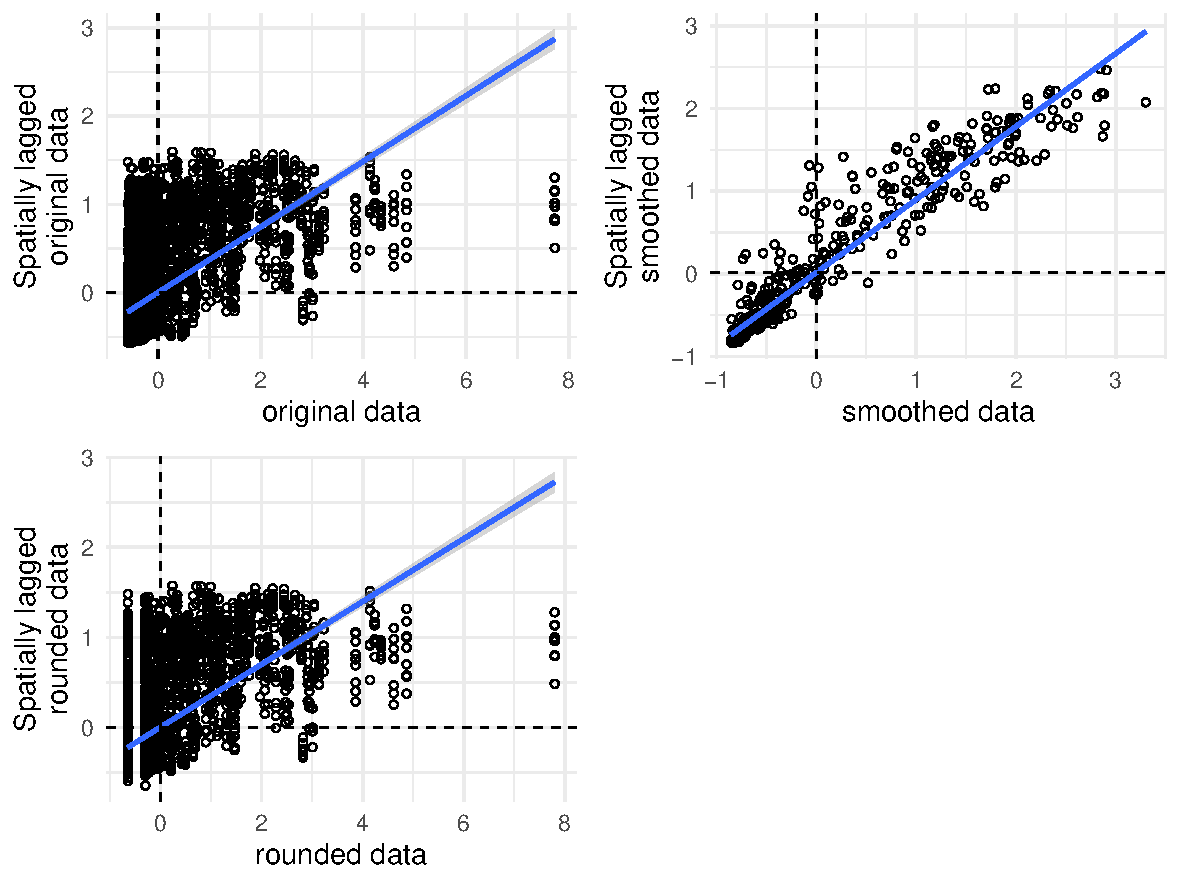
\includegraphics[width=0.8\linewidth]{figures/moran_plot.pdf}
    \caption{Moran's diagrams applied on the number of poor households, with the original data, the data protected by a smoothing method and by a rounding. Be aware that the axes do not have the same scales.}
    \label{fig:moran_plot}
\end{figure}

\section{Local Information Loss} \label{sec:util_LOC}

In sections \ref{sec:util_DD} and \ref{sec:util_SPAT} the metrics discussed were \emph{global}, in the sense of yielding a single aggregate number of information loss for a whole map. Such high-level aggregates often do not capture nuanced distortions, that may nevertheless be relevant to certain data uses \citep{CoxEtAl2011, WooEtAl2009}.
Trivially, if all the distortion occurs in a single small part of the map, the overall information loss may be judged low. But a user specifically interested in that part would nevertheless face a severe inhibition of the maps utility. It is therefore usually a good idea to complement aggregate information loss metrics with \emph{local} measures.

\subsection{Mapping the spatial distribution of error} \label{sec:util_LOC_cellerror}

One way to gain local measures is to `disentangle' global measures and map their individual contributions. In other words, to create a map, where each grid cell displays its individual error value. This allows analyzing the spatial distribution of error. Cell-level measures for the global metrics introduced in \ref{sec:util_DD_hd} are shown in Table \ref{tab:util_cellLVL}.
%\footnote{
    %The cell-level measure pertaining to the Hellinger distance (Eq. \ref{eq:util_hd}) is the squared distance of square roots (SDSR), while the squared error (SE) and absolute error (AE) are the localized parts of the mean squared error (Eq. \ref{eq:util_mse}) and mean absolute error (Eq. \ref{eq:util_mae}) respectively; see \cite{AntalEtAl2017}.}
An example is visualized in Fig. \ref{fig:LErr_maps} (bottom left).

\begin{table}[H]
    \centering
    \begin{tabular}{l c c}
    \hline
    Cell-level measure & Equation & Aggr. measure \\
    \hline
        \rule{0pt}{18pt} Squared dist. of sqr. roots (SDSR) &  $\left(\sqrt{X'_j} - \sqrt{X_j}\right)^2$ & HD \\
        \rule{0pt}{18pt} Squared error (SE) & $\left(X'_j - X_j\right)^2$ & MSE  \\
        \rule{0pt}{18pt} Absolute error (AE) & $\left|X'_j - X_j\right|$ & MAE  \\
        \hline
    \end{tabular}
    \caption{Local information loss metrics based on distributional distances; see also \citet{AntalEtAl2017}.}
    \label{tab:util_cellLVL}
\end{table}

Local information loss measures based on spatial association include the absolute difference in \emph{local} Moran's $\mathcal{I}$ as per Eq.(\ref{localI}) and the absolute difference in local spatial correlation as per Eq.(\ref{eq:dM_i}). Both were introduced in section \ref{sec:util_moran}.

\subsection{Moving window approach / focal error} \label{sec:util_LOC_mw}

A moving window method, also sometimes called \emph{focal statistic}, is a general-purpose grid processing technique, where a value is assigned per grid cell based on the values in that cell's neighborhood. Conceptually, think of a window as a frame of some intermediate size (say, 15 $\times$ 15 cells), symmetrically centered on a single cell, which we call the \emph{focal cell}. The focal cell gets assigned a value that is a function of the $15 \cdot 15 = 225$ cell values currently within the window, but not depending on any values outside of it. \citet{KuhnertEtAl2005} explain how moving window methods may be used for measuring the dissimilarity between grid maps.

In our case, the idea is to assign the focal cell an information loss measure. Specifically, one of the global measures listed above, but computed only based on the cells within the window (therefore `localized'). Straightforward picks are the Hellinger distance (HD), Mean Squared Error (MSE), or Mean Absolute Error (MAE) from section \ref{sec:util_DD_hd}. For example, when using the MAE, the absolute errors are calculated for all, say $225$ cells in the window and their mean is assigned to the focal cell. Subsequently, the window is shifted one cell over and the procedure is repeated.\footnote{
    Moving window methods are typically applied to rectangular grids, either row-wise or column-wise. When the end of a row / column is reached, the window is shifted to the next, until all cells in the grid have been processed.}
The size of the window determines the degree of `localism': the smaller the window, the more local the measure. The moving window approach can therefore implement different levels of `compromise' between global information loss measures (as per \ref{sec:util_DD} and \ref{sec:util_SPAT}) and mapping the cell-level error (as per \ref{sec:util_LOC_cellerror}).

An example is shown in Fig. \ref{fig:LErr_maps} (bottom right). Compared to the cell-level error in Fig. \ref{fig:LErr_maps} (bottom left), the moving window method marks regions of the map where either many cells with some error or a few cells with large error lie together. The parts of the map most impacted should thus be noticeable at a glance.\footnote{
    Note that the size of the region impacted needs to be viewed in conjunction with the size of the error. For instance, in Fig. \ref{fig:LErr_maps} (bottom right), the MAE over 1.5km $\times$ 1.5km chunks is mostly below 5 and in the most afflicted regions %(ca. 1\% of the map) 
    between 5 and 10.}

\begin{figure}
    \centering
    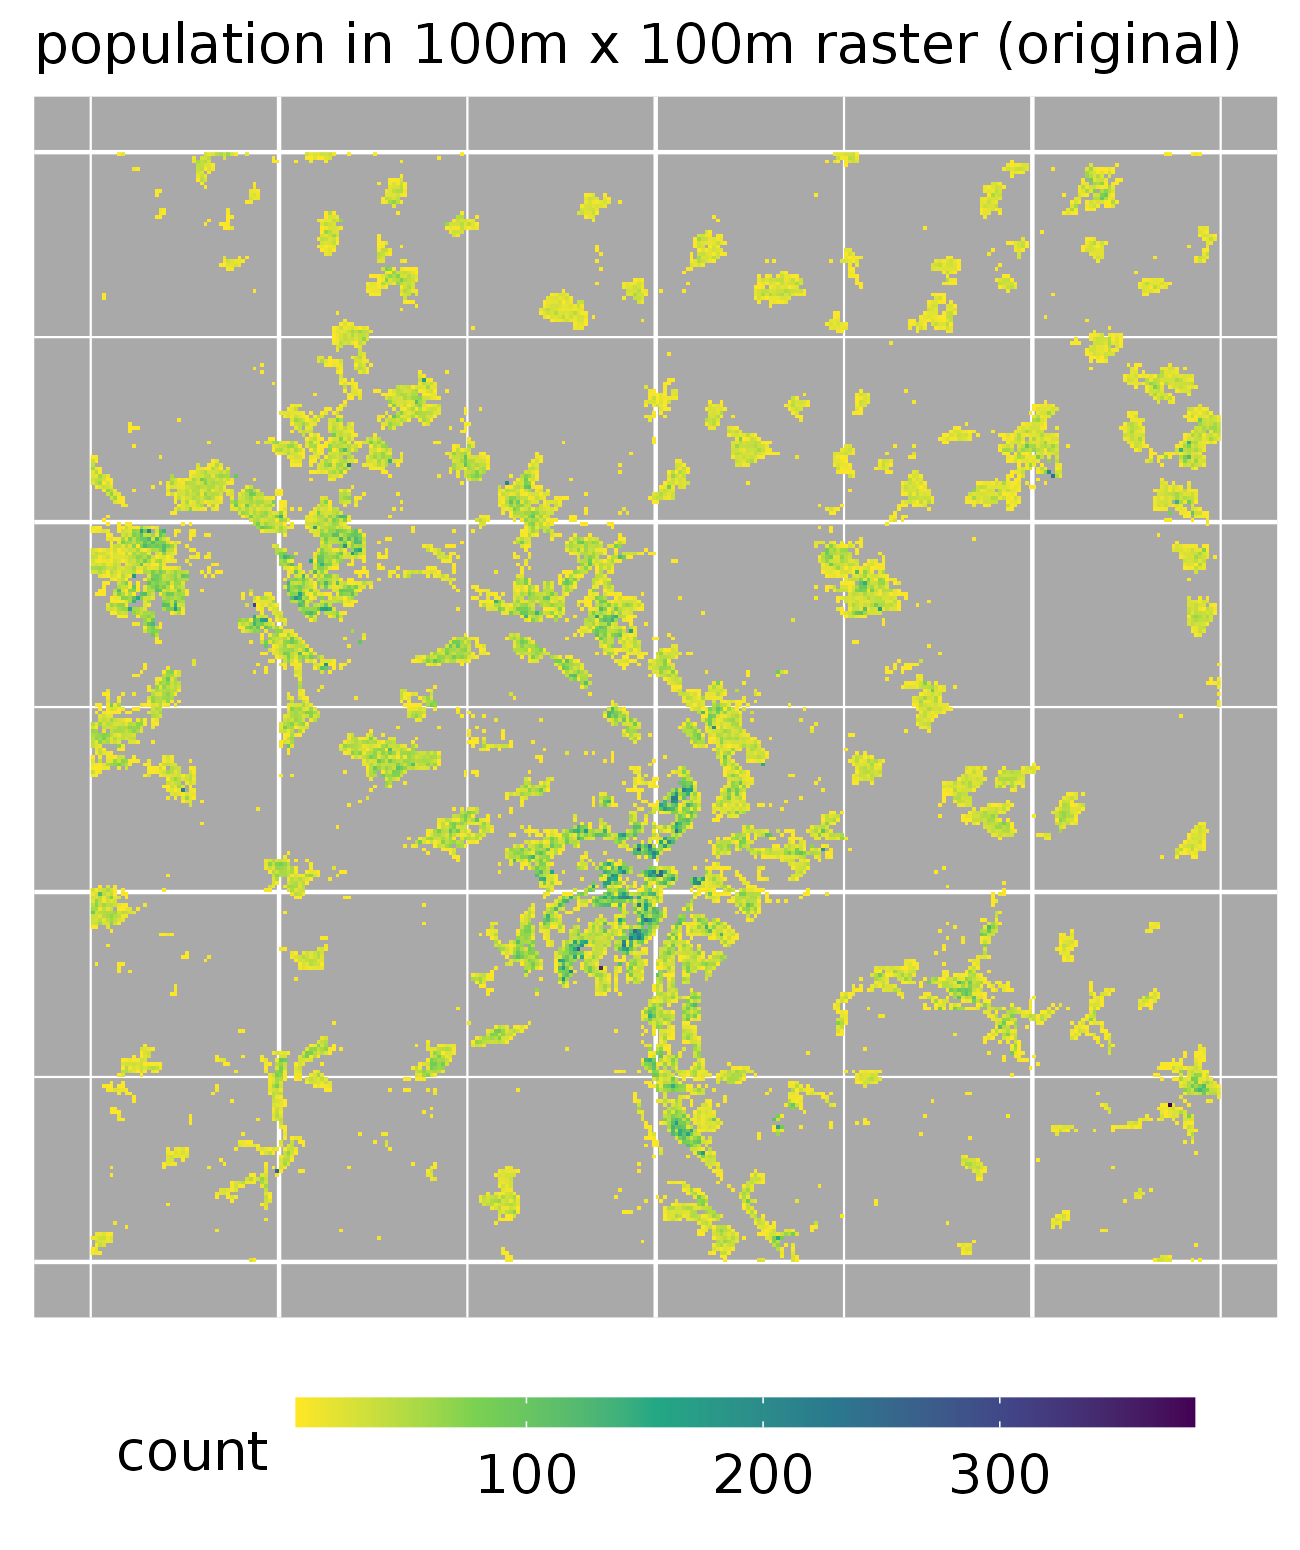
\includegraphics[width=.49\linewidth]{figures/lerr_map_orig.png}
    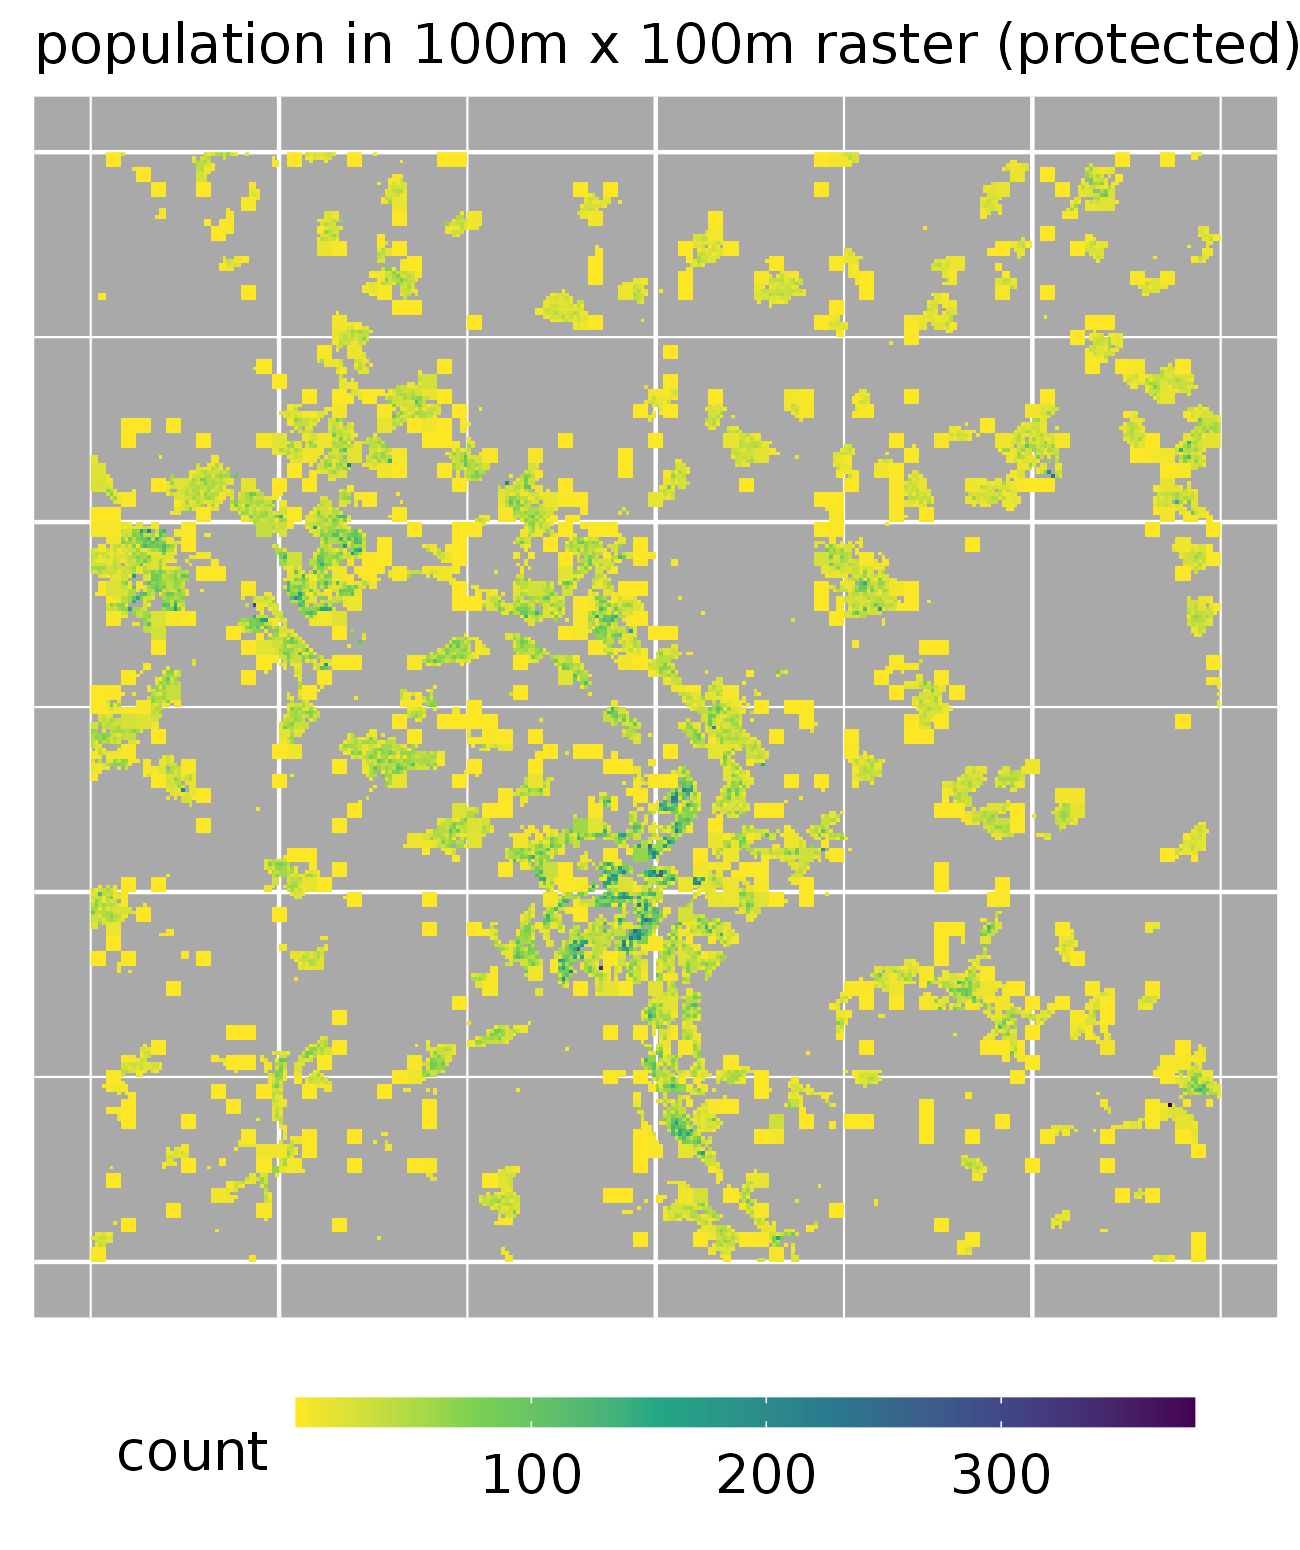
\includegraphics[width=.49\linewidth]{figures/lerr_map_prot.png}
    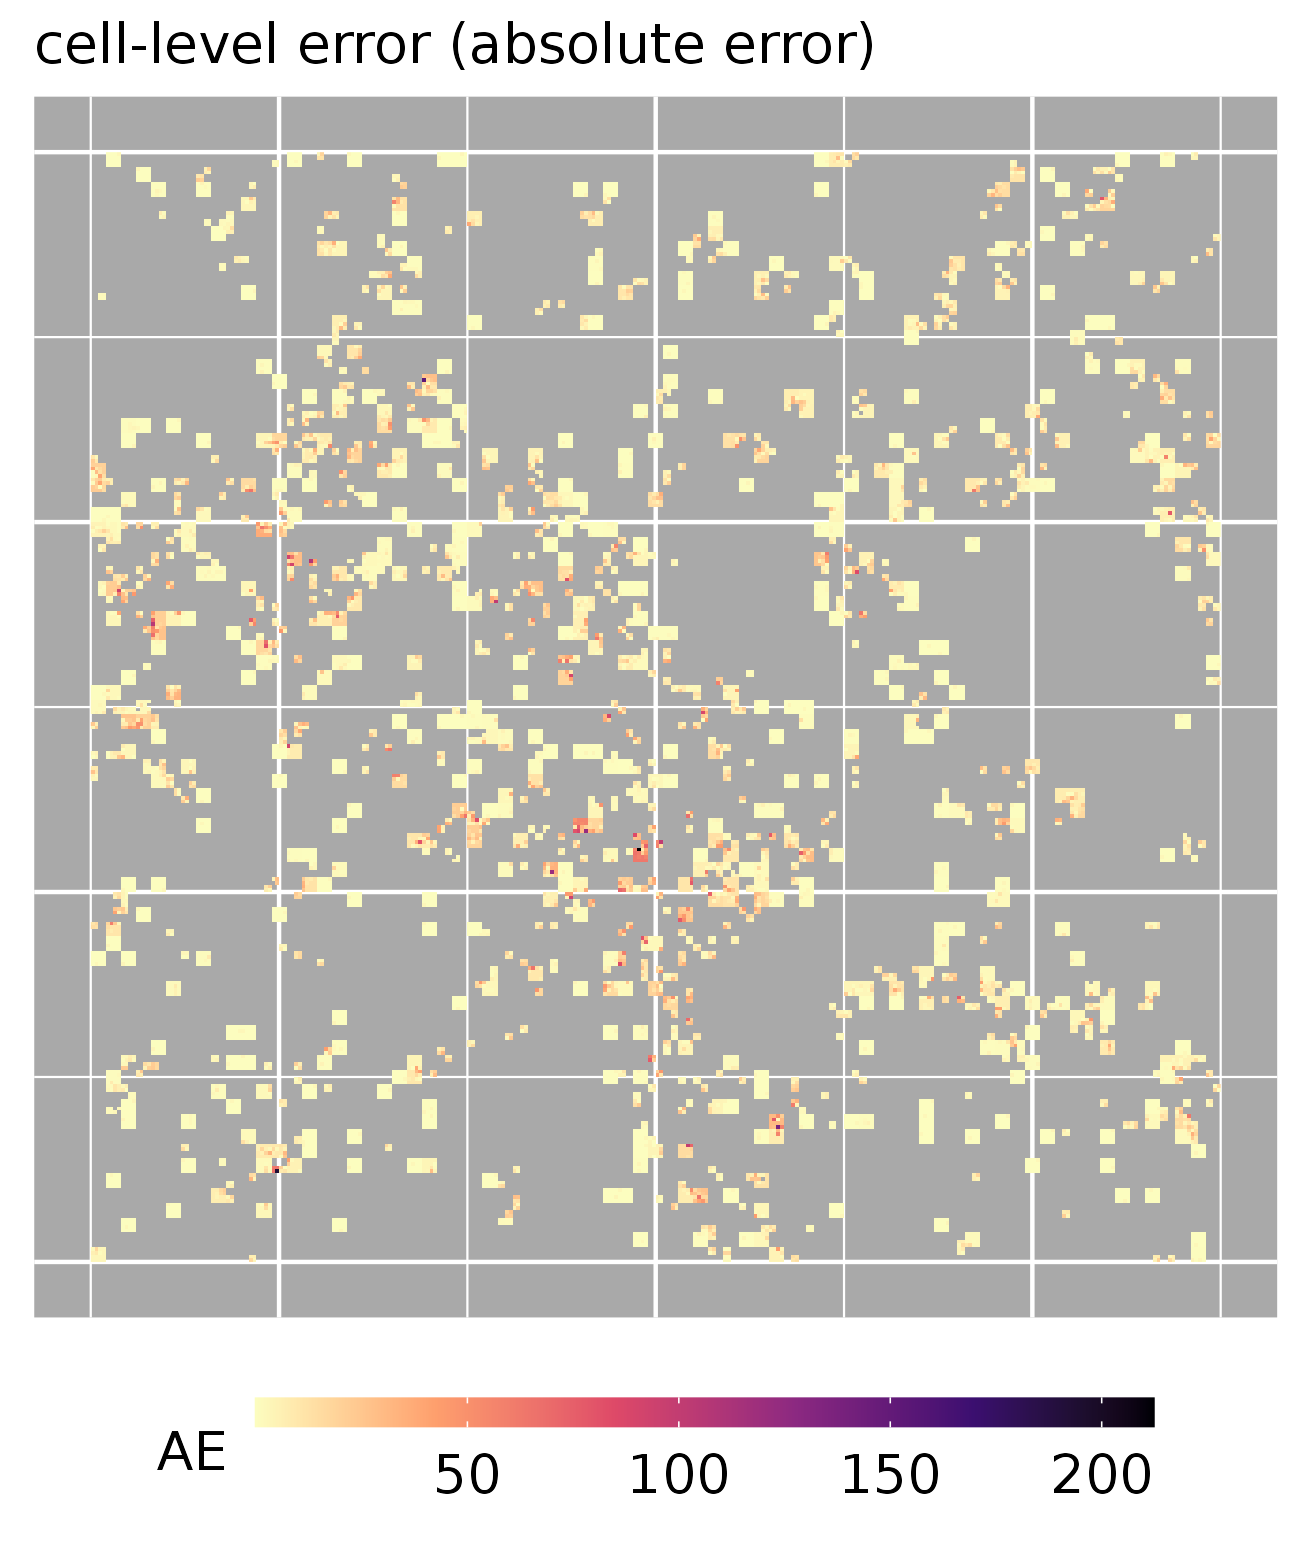
\includegraphics[width=.49\linewidth]{figures/lerr_map_ae.png}
    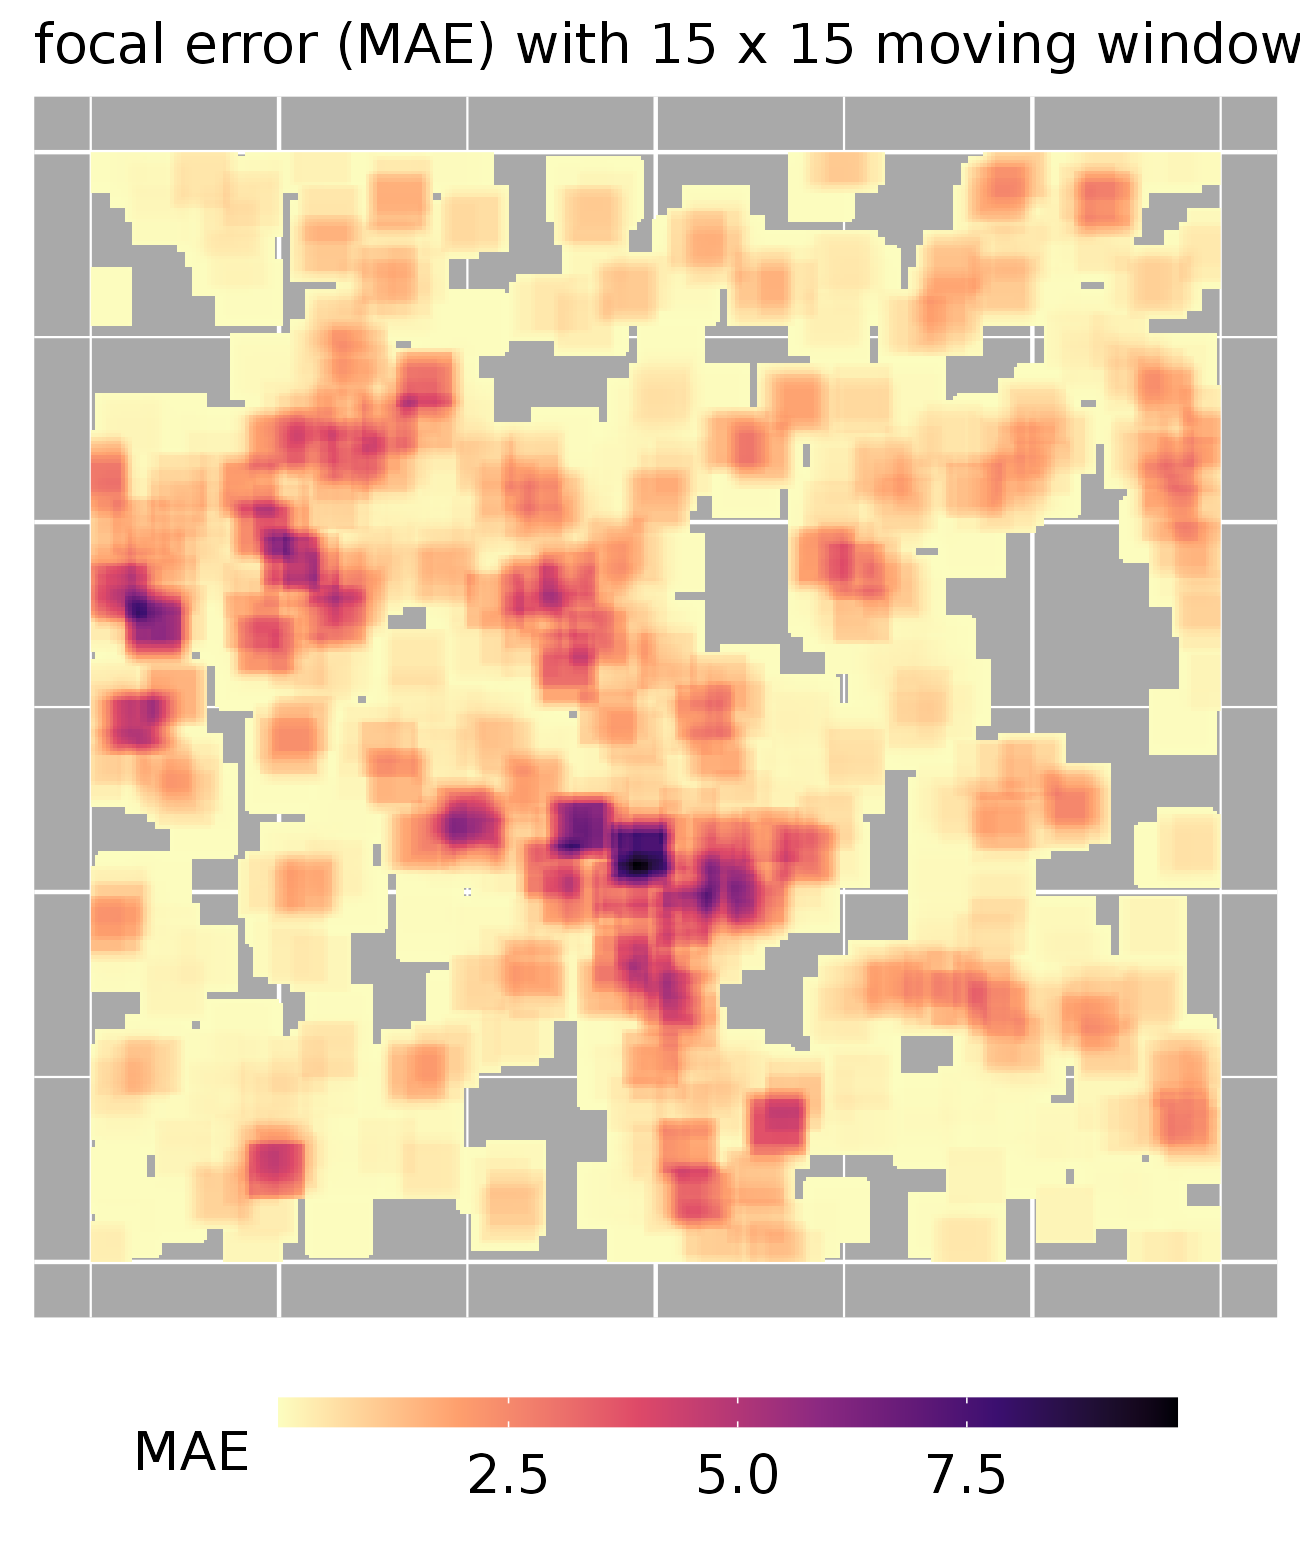
\includegraphics[width=.49\linewidth]{figures/lerr_map_mw_mae.png}
    \caption{Maps of local information loss; top: original map containing small counts (left) and protected map (right) (protection via quadtree algorithm); bottom: cell-level error map with AE measure (left) as per Table \ref{tab:util_cellLVL} and corresponding focal error map of MAE with the moving window method (right) using a window of size 15 $\times$ 15 grid cells.}
    \label{fig:LErr_maps}
\end{figure}


\section{Information Loss Measures and the Modifiable Areal Unit Problem}


Spatial data analysis faces a classical problem known as the Modifiable Areal Unit Problem (MAUP), which denotes two associated sub-problems regarding how spatial data are geographically aggregated:

\begin{itemize}
    \item The zoning effect refers to the sensitivity of results to how the different zones in which the data are grouped are delineated.
    \item The scale effect refers to the geographic precision level of the zoning used: studying a spatial phenomenon at a regional scale may not necessarily lead to the same conclusions as studying it at a municipal scale.
\end{itemize}

\paragraph{Does this problem also concern the data protection stage?}

Actually, any method that influences the delineation of initial geographic areas, primarily by aggregating them, is concerned. Indeed, aggregating two zones to manage a confidentiality issue necessarily generates a zoning problem (the result is sensitive to the chosen zones) and a scale problem (spatial analysis cannot be conducted at the same scale across the entire territory). In this case, information loss measures, especially those based on spatial auto-correlation as the Moran’s $\mathcal{I}$, could be less relevant to compare maps before and after the treatment. Indeed, the comparability of the measures can be lost if the neighbourhoods of the tiles, which the computation of Moran's $\mathcal{I}$ is based on, are modified by the protection process.

Among the methods presented in the chapter~\ref{sec:methods}, only the quadtree method is likely to modify the original level of resolution by aggregating tiles when the confidentiality threshold is not reached (see section~\ref{sec:quadtree}). This modification makes the method sensitive to the zoning effect (since the analysis will be sensitive to the way in which the tiles are aggregated) and to the scale effect (notably because not all tiles will have the same level of resolution). As the Moran’s $\mathcal{I}$ calculation requires to define the neighborhood of each tile, modifying these tiles (by aggregating some of them, for example) modifies their neighborhood (Figure~\ref{fig:queen_neigh}) and, then, makes measurements difficult to compare.

\begin{figure}
    \centering
    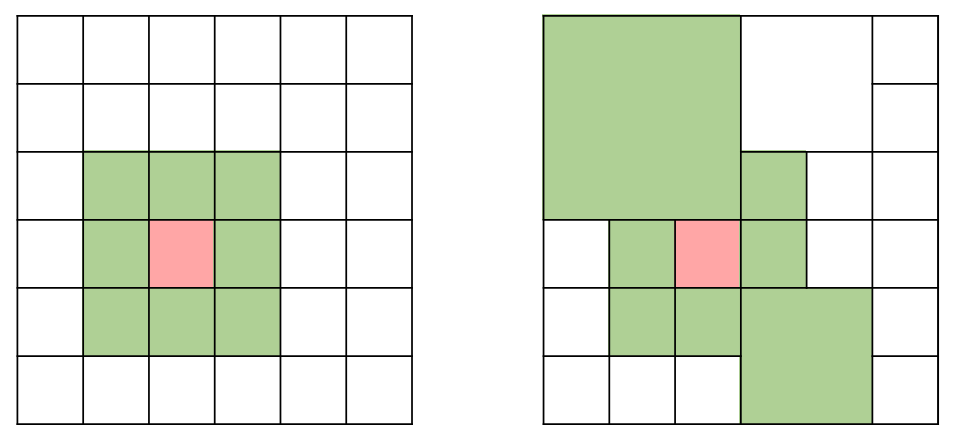
\includegraphics[width=0.75\linewidth]{figures/queen_neighborhood.png}
    \caption{Queen neighborhood (green tiles) of the red tile in the case of a regular grid (left) or an irregular one (right)}
    \label{fig:queen_neigh}
\end{figure}

\paragraph{Another question to ponder is: at what geographic scale should the original and protected maps be compared?}

Users are invited to measure utility (or information loss) at a relevant scale based on the disseminated data and anticipated analyses.

As the information loss cannot be expected to be identical at a global scale (e.g. country level) and at any intermediate or small scale (e.g. region or municipality level), the person in charge of data protection should adapt the scale at which they measure the information loss due to the application of protection methods, depending on the intended uses.

%Let's take the example of the number of households living on the island of La Réunion (France) in 2019. The counts are disseminated in a grid of $200$m $\times$ $200$m tiles. If we compute the Moran's I at the scale of the island, we obtain a Moran's I of $0.521$. But if we calculate Moran's I in each 16km x 16km tile encompassing the island, we obtain a Moran's I ranging from 0.26 to 0.53 depending on the studied area (excluding parts of the island with less than 100 200m tiles).



\chapter{Disclosure Control Methods for Geo-Referenced Data} \label{sec:methods}
\chaptermark{Methods}
    \section{Quadtree-based methods}\label{sec:quadtree}

Today, the dissemination of gridded data is becoming widespread, as it allows for adjusting the scale at which information is made available. Additionally, a grid is a purely geometric and regular partitioning independent of administrative boundaries. Gridded data generally allows for better consideration of scale and zoning effects underlying the Modifiable Areal Unit Problem (MAUP) theorized by \cite{openshaw1979million}.

However, gridding also provides an opportunity to disseminate information about increasingly smaller geographical areas. For example, Insee (French National Institute of Statistics and Economic Studies) disseminates certain tax information on grids of 200m square\footnote{\url{https://www.insee.fr/fr/statistiques/7655475?sommaire=7655515} (in French)}, and all European statistical institutes are preparing to disseminate population data from the 2021 Census on 1km $\times$ 1km grids. This increases the risks of reidentification or disclosure of sensitive attributes. Without adequate protection methods, the dissemination of such data would not be possible.

To mitigate the risks of disclosure, a population threshold is generally set so that below it, information is considered sensitive or confidential and must be treated.

Among the non-perturbative methods available to the producer, \citet{Strobl_2005}, for the dissemination of Austrian Census data, and \citet{Behnisch_Meinel_Tramsen_Diesselmann_2013}, for the Leibniz Institute, have proposed using the so-called \emph{quadtree method} to protect gridded data from the risk of disclosing confidential information. This technique has also been implemented by \citet{Lagonigro_Oller_Martori_2017} and \citet{Suñé_Ibáñez_2017} for the Statistical Institute of Catalonia, and a variant is used by Insee \citep{Branchu_Costemalle_Fontaine_2018} for the dissemination of tax data and Census 2021 results.


\subsection{The aggregation process}

The Quadtree is primarily a space subdivision technique proposed by \cite{hunter1978efficient} and further developed by \cite{Samet_1984}, which relies on a hierarchical structure of space in the form of nested grids of increasingly larger resolutions.

\begin{tcolorbox}[breakable]
Taking an example from \cite{Lagonigro_Oller_Martori_2017}, shown here as Fig.~\ref{fig:subdivision_quadtree}, $A$ represents the maximum extent of the map as a single grid. The size of this grid defines the lowest possible resolution. This grid is subdivided into $4$ grids of medium resolution ($B$, $C$, $D$, and $E$), and $C$ is further subdivided into 4 grids of maximum resolution ($F$, $G$, $H$, and $I$). This decomposition can also be represented as a hierarchical tree, hence the name of the method.

%\begin{figure}
    %\centering
    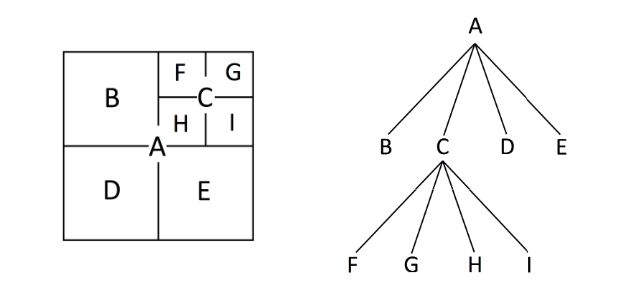
\includegraphics[width=0.8\linewidth]{figures/Quadtree/space_subdivision_lagonigro_fig1.png}
    \captionof{figure}{Subdivision of space and its equivalent quadtree representation (Source: \cite{Lagonigro_Oller_Martori_2017}, p. 144).}
    \label{fig:subdivision_quadtree}
%\end{figure}
\end{tcolorbox}

As a data protection technique, the quadtree involves disseminating each non-confidential information at the highest desired resolution level. The hierarchical tree can be built using two types of approaches:
\begin{itemize}
\item A \emph{bottom-up} approach, by far the most common, starting from the maximum resolution level (the leaves of the tree) and aggregating grids in the presence of confidential information;
\item A \emph{top-down} approach would start from the minimum resolution level (root of the tree) and decompose each grid until a confidential information is disclosed.
\end{itemize}

\cite{Behnisch_Meinel_Tramsen_Diesselmann_2013} and \cite{Lagonigro_Oller_Martori_2017} both use a fairly similar bottom-up approach.

We will use the example presented in Figure~\ref{fig:quadtree_aggregation} to detail the steps of the aggregation algorithm. We assume that the territory is divided into four levels of resolution: 250~m $\times$ 250~m (resolution 1, thin gray lines), 500~m $\times$ 500~m (resolution 2, thin black lines), 1~km $\times$ 1~km (resolution 3, thick black lines), and 2~km $\times$ 2~km (resolution 4, thick blue lines). This example is adapted from Figure 14.2 in \citet[p.358]{BuronFontaine2018}. In this example, the confidentiality threshold is set to $3$: each cell must contain at least three individuals to be disseminated.

\begin{figure}
    \centering
    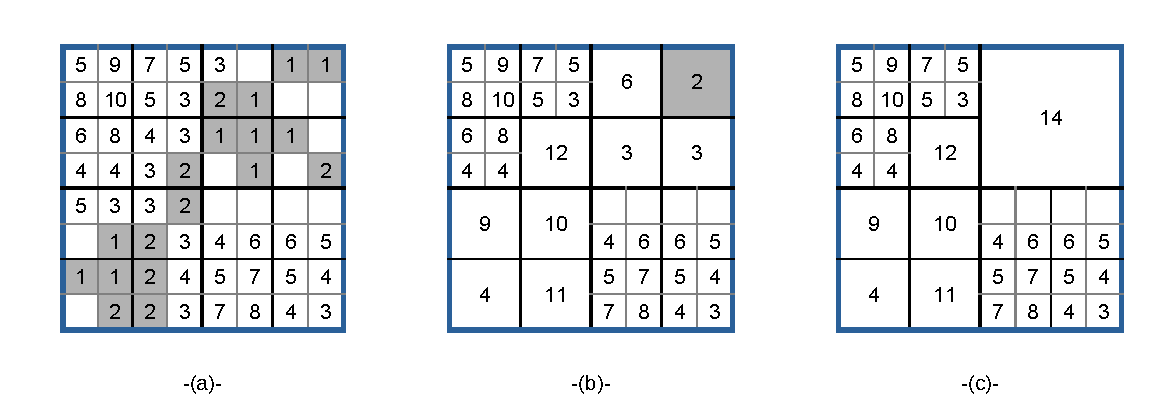
\includegraphics[width=1\linewidth]{figures/Quadtree/adaptation_example_handbook_spat_ana.pdf}
    \caption{Quadtree aggregation with a bottom-up approach (confidentiality threshold $=3$) - adapted from \citet[p.358]{BuronFontaine2018}}
    \label{fig:quadtree_aggregation}
\end{figure}

\begin{itemize}
    \item First, the information is distributed in the grid with the finest possible resolution (resolution 1, Figure~\ref{fig:quadtree_aggregation} (a)). All cells containing confidential information are identified (gray cells).
    \item Each confidential cell is aggregated with the other three cells belonging to the same resolution 2 cell. Thus, at the bottom left, the information is no longer disseminated at resolution 1 but will be at best at resolution 2 (Figure~\ref{fig:quadtree_aggregation}, (b)).
    \item Since there is still a resolution 2 cell below the confidentiality threshold (top right), it is necessary to aggregate this cell with the other three cells belonging to the same resolution 3 cell (Figure~\ref{fig:quadtree_aggregation}, (c)).
    \item The grid (c) no longer contains confidential information and can be disseminated.
\end{itemize}

\subsubsection{Choice of the grid and anchoring of the hierarchical structure}

The quadtree approach relies on a hierarchical structure of grid cells. This means that this method can only be applied if the areas of a specific resolution are perfectly nested within each of the areas of higher resolutions. For example, a quadtree can't be achieved with a $200$~m and a $500$~m grid at the same time, because not all the $200$~m squares are entirely contained in a $500$~m square.\bigskip

Although a strict quadtree approach consists of splitting each square into four smaller squares, it is possible to design a variant that first chooses the size of the different resolution levels and then applies a quadtree to all the chosen resolutions. For example, it is possible to adapt the methodology so as to release $100$~m squares as the lowest resolution, and $500$~m and $1$~km squares as intermediate resolutions if necessary. In this case, with a bottom-up approach, within a given $500$~m square, the information is released at the $100$~m resolution if and only if all of the twenty-five $100$~m squares are above the threshold.\bigskip

In addition, the result of the aggregation process is highly dependent on the anchoring of this hierarchical structure. A slight shift in one or more directions can have significant consequences for the method's output. Based on the example presented earlier (Fig.~\ref{fig:quadtree_aggregation}), suppose we keep exactly the same population per cell (finest grid in gray) but shift the anchoring of the hierarchical structure (black lines, dark black, and thick blue) by one cell downwards and one cell to the right. The new aggregation process is shown in Figure~\ref{fig:quadtree_pos_grid}. It can be observed that this leads to very different results, requiring, in particular, the aggregation of two very large cells (bottom left and top right), resulting in significant information loss.

\begin{figure}[ht]
    \centering
    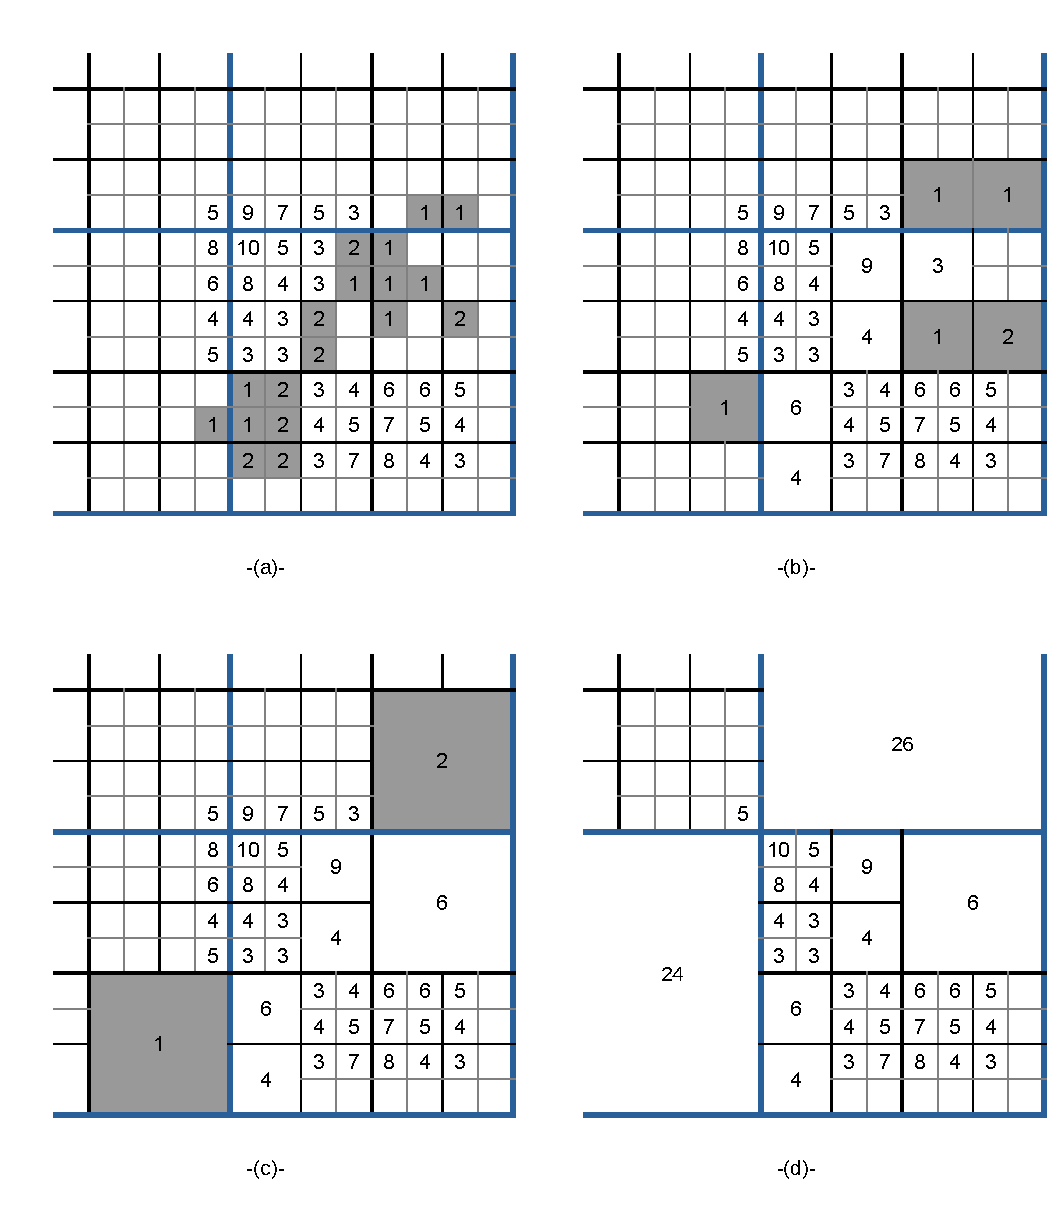
\includegraphics[width=0.89\textwidth]{figures/Quadtree/adaptation_example_variante_pos_grid.pdf}
    \caption{Quadtree applied on the same population as in Fig.~\ref{fig:quadtree_aggregation}, but with a different anchoring of the hierarchical structure}
    \label{fig:quadtree_pos_grid}
\end{figure}

One could consider testing several positions of the hierarchy (but taking also the  spatial hierarchy formally assumed for publication purposes into account) and choosing the one that leads to the minimal information loss. However, such a solution would have the major drawback of making maps (for example, from one year to another) impossible to compare. In the context of a single study, this option could be considered, but it does not seem realistic for the work of a statistical institute.

Instead, it is more beneficial, following the examples of \cite{Behnisch_Meinel_Tramsen_Diesselmann_2013} and \cite{Lagonigro_Oller_Martori_2017}, to use the INSPIRE grid coding standard. This standard ensures perfect stability of the grid cells and their hierarchical structure. This allows tools such as the R packages \texttt{sdcSpatial} \citep{sdcSpatial_2022} and \texttt{AQuadtree} \citep{AQuadtree_2023} to provide stable results. However, this choice does not guarantee the minimization of information loss during the quadtree process.


\subsubsection{Resolution Levels}

The bottom-up approach begins with a maximum resolution level, i.e., with the smallest tiles desired by the producer. The method iteratively changes the resolution level of the information to be disseminated as long as there is confidential information remaining. The classic choice is to select a resolution twice as low at each iteration: starting with tiles of $250$~m, the next level would consist of tiles of $500$~m, then $1$~km, and so on. This is the choice made by \citet{Behnisch_Meinel_Tramsen_Diesselmann_2013} and \citet{Lagonigro_Oller_Martori_2017}, and it is the one implemented in \citet{sdcSpatial_2022} as well as \citet{AQuadtree_2023}. In this case, each tile at a higher level consists of exactly 4 tiles at the lower level. However, in theory, there is no restriction on pre-selecting resolution levels. For example, Insee has chosen a maximum resolution of $200$~m $\times$ $200$~m, with the higher level being $1$~km $\times$ $1$~km. This higher level thus contains $25$~tiles of $200$~m, which may lead to a more significant local information loss than with a classic hierarchy.

In the absence of pre-defined stopping criteria, the aggregation process will continue as long as a tile contains confidential information. The R package \texttt{sdcSpatial} \citep{sdcSpatial_2022} suggests setting the minimum acceptable resolution level. It is therefore possible to choose to stop the aggregation process before all confidential cells are processed, with a complementary (suppressive or perturbative) method being considered additionally.

\subsubsection{Extreme Cases of Aggregation}

Setting a minimal acceptable resolution level turns out to be a good idea to prevent some rare but extreme situations from excessively altering the data's utility. Figure~\ref{fig:quadtree_reunion} shows a quadtree applied to household numbers on the French island of La Réunion. This volcanic island has its population mainly located on the coast. 

The quadtree is applied starting from a $200$~m grid, then a $1$~km, $2$~km grid, and so on. However, applied without a stopping criterion, we observe that the aggregation process leads to the formation of $3$ tiles of $16$~km each, with an average of over $17,000$ households. The information loss is significant and is actually due to very specific configurations. The case of the tile surrounded in red is presented in Figure~\ref{fig:quadtree_reunion_issue}, where the $1$~km tiles have been represented, along with the $4$~tiles of $8$~km composing the red tile in Figure~\ref{fig:quadtree_reunion}. It can be observed that the southeast quarter consists of only two $1$~km tiles, each containing at most $4$~households. In total, these two tiles count at most $8$~households, which is below the authorized dissemination threshold of $11$~households.\footnote{
    We reassure the reader that in reality this information is not confidential and can be used here for demonstration purposes.}

Thus, aggregating these two tiles at the $8$~km resolution level is not sufficient and requires aggregation at a lower resolution level ($16$~km). However, it turns out that this tile is adjacent to a densely populated area, resulting in the complete loss of detail of the dense part of this area.

\begin{figure}[H]
\begin{minipage}{0.48\linewidth}
    \centering
    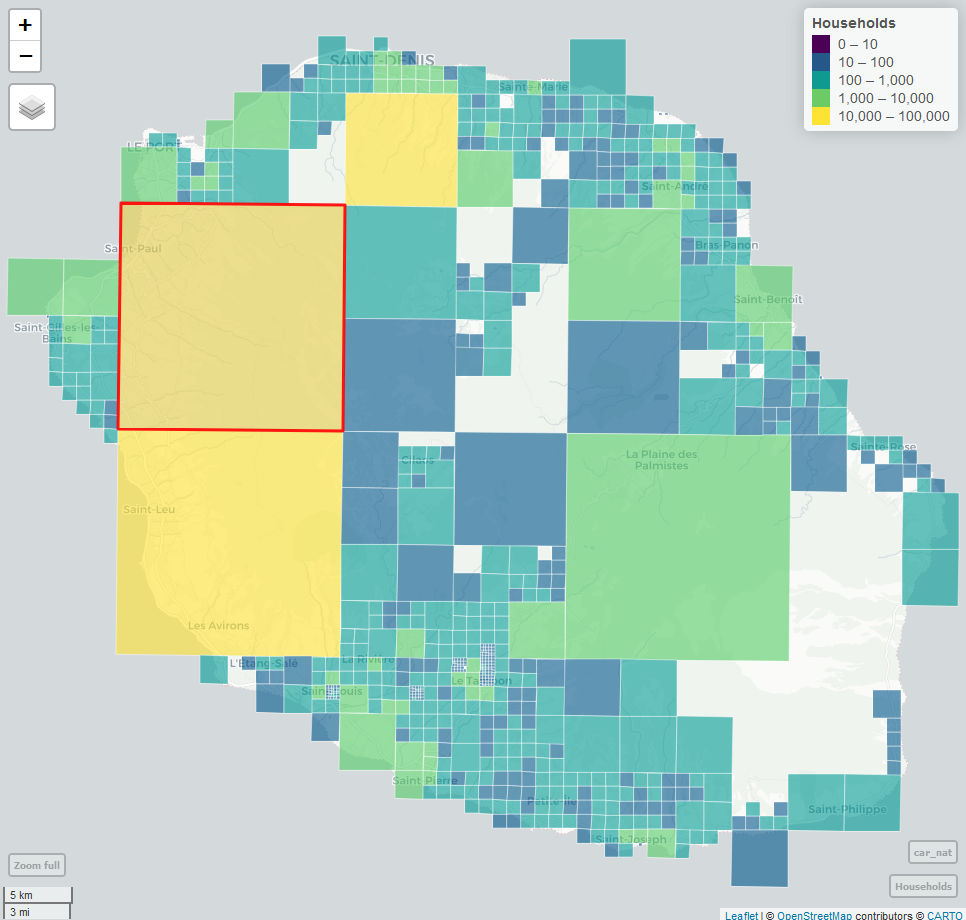
\includegraphics[width=\linewidth]{figures/Quadtree/reunion_quadtree_filo2019.png}
    \caption{Quadtree approach applied on household numbers in La Réunion (France)}
    \label{fig:quadtree_reunion}
\end{minipage}
\hfill
\begin{minipage}{0.48\linewidth}
    \centering
    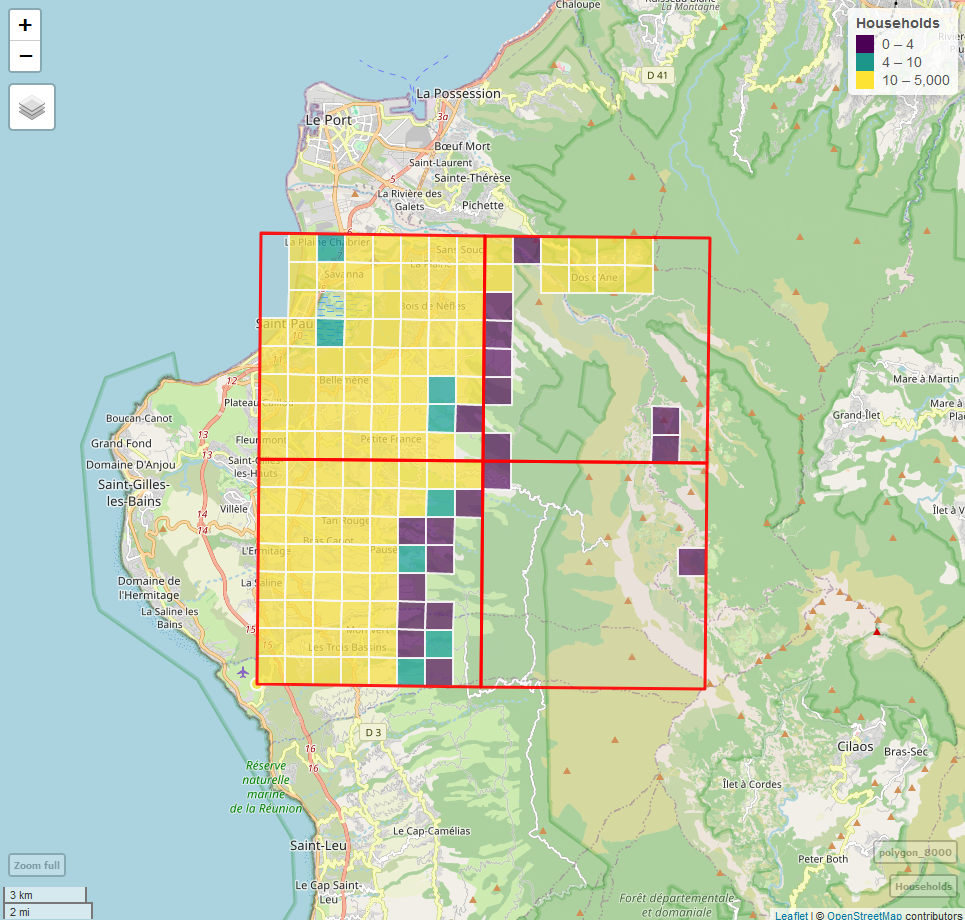
\includegraphics[width=\linewidth]{figures/Quadtree/reunion_quadtree_filo2019_issue.png}
    \caption{Quadtree issue in extreme case\\ \ }
    \label{fig:quadtree_reunion_issue}
\end{minipage}
\end{figure}

\begin{table}[H]
\footnotesize
\centering
\begin{tabular}[t]{rrrrrr}
\toprule
\multirow{2}{*}{Size of squares (meters)} & \multicolumn{2}{c}{Squares} & \multicolumn{3}{c}{Households} \\
\cmidrule{2-3} \cmidrule{4-6}
 & NB & \% & Total & \% & Mean \\
\midrule
200 & 157 & 22 & 9~662  &  3 & 62\\
1~000 & 447 & 64 & 17~8400 & 55 & 399 \\
2~000 & 64 & 9 & 32~074 & 10 & 501 \\
4~000 & 29 & 4 & 30~747 & 10 & 1~060\\
8~000 & 6 & 1 & 19~373 & 6 & 3~229\\
\addlinespace
16~000 & 3 & 0 & 52~408 & 16 & 17~469\\
ALL & 706 & 100 & 322~664 & 100 & 457\\
\bottomrule
\end{tabular}
\caption{Results of the quadtree process on households frequencies in La Réunion}
\label{tab:quadtree_reunion_summary}
\end{table}


Such cases justify an approach consisting of setting a minimal resolution level, even if it means having to deal separately with the untreated confidential tiles. A suppressive method, consisting of removing the information from the remaining confidential tiles ,is a feasible option (see section \ref{sec:aux_suppr}). The information loss is generally not significant, since it concerns only tiles below the confidentiality threshold. \citet{Lagonigro_Oller_Martori_2017} and \citet{Suñé_Ibáñez_2017} choose to randomly relocate the population of these tiles. \citet{Suñé_Ibáñez_2017}, in particular, demonstrates the usefulness of this approach in terms of utility through simulation studies.


\subsection{Utility Aspects}

% Show that utility decreases with the aggregation level
Using the Hellinger distance (see \ref{sec:util_DD_hd}) or the Kantorovich-Wasserstein distance (see \ref{sec:util_DD_kwd}), \cite{GussenbauerEtAl2023} demonstrated on several examples that at the same protection level, the quadtree method resulted in a stronger loss of information compared to a method of removing cells containing confidential information, but less significant than smoothing.

By choosing a minimal resolution level in advance, the same article shows the expected effect on utility: by allowing the aggregation of confidential cells at an additional level, the Hellinger distance increases significantly in most cases. This experimentation illustrates the importance of setting a minimal resolution level as a stopping criterion for the aggregation process to maintain good utility. However, such a choice requires additional measures to protect any remaining confidential cells.

\subsubsection{Quadtree and Spatial Analysis}

Spatial autocorrelation is an essential element of spatial analysis. To provide useful spatial data, care must be taken to ensure that the protection mechanism does not overly alter the intensity of the initial autocorrelation. However, the quadtree, by aggregating certain cells, will distort the intrinsic neighborhood relationships. Let's take the example of households residing on the island of La Réunion (Fig.~\ref{fig:quadtree_reunion}). After aggregation, Moran's $\mathcal{I}$ (see section \ref{sec:util_moran}) is $0.228$, whereas it was $0.555$ on the original data for a $1$~km grid (Tab.~\ref{tab:MoranI_reunion}). Worse, using Euclidean distance to define neighbor weights, Moran's $\mathcal{I}$ becomes very close to $0$ ($0.050$). Although the statistic remains significantly different from zero, the data disseminated with the quadtree method reduces the importance of the observed spatial autocorrelation.

Such distortion can be controlled by avoiding extreme cases of aggregation, especially by limiting the acceptable minimal resolution level and separately processing the remaining extreme cases (see above). Limiting the minimal resolution level will also prevent the reappearance of scale issues (MAUP) in data analysis.

\begin{table}
    \centering
    \begin{tabular}{ccc}
        \toprule
        \multirow{2}{*}{Release} & \multicolumn{2}{c}{Moran's $\mathcal{I}$} \\
        \cmidrule{2-3}
                                 & Queen Neighbor & Euclidian distance\\
        \midrule
        original 1km grid        & 0.555          & 0.331 \\
        maximal quadtree         & 0.228          & 0.050 \\
        \bottomrule
    \end{tabular}
    \caption{Moran's $\mathcal{I}$ applied on household frequencies in La Réunion, depending on the release and the way to define the neighborhood.}
    \label{tab:MoranI_reunion}
\end{table}
% All test statistics are significant at the 5% level.

\subsubsection{How to Disseminate Multiple Variables on Comparable Maps?}

The quadtree is theoretically a method to be applied separately for each variable we want to disseminate. However, there is no guarantee that the process will lead to the same result in terms of aggregation. Worse, it is even expected that the results will be different. Thus, maps become hardly comparable and lose their utility. What should we do, if we want to disseminate maps of total population, female population, and male population in a given territory and allow comparability of published maps?

\cite{Lagonigro_Oller_Martori_2017} propose setting a second threshold they call the \emph{anonymity threshold}, in addition to the \emph{aggregation threshold}. The latter determines whether the tiles should be aggregated or not, while the former specifies whether attribute information can be disseminated or not. If a tile meets the aggregation threshold but not the anonymity threshold for one of its attributes, the overall information (total population) is then disseminated but the information on the attribute in question is to be suppressed. A secondary suppression is also necessary to avoid differencing with margins. Thus, a suppression step is applied to the attributes.

For example, let's suppose that in a given tile there are $10$~inhabitants, of which $2$ are men. Suppose further that the aggregation level is set to $9$ and the anonymity threshold to $3$. In this case, the aggregation process won't aggregate the tile to a lower resolution level and the total population of the tile will be disseminated. But the number of men won't be released, because it is below the anonymity level. In order to avoid any margin differencing, one has to suppress the counts of females too.

 For the authors, this anonymity threshold applied to attributes ensures a protection level compliant with $k$-anonymity. It is actually an extensive version of $k$-anonymity, where all disseminated attributes would be considered quasi-identifiers.

The disadvantage of this method is that it requires choosing two thresholds, the aggregation threshold having to be higher than the anonymity threshold of the attributes. For example, it is possible to choose an aggregation threshold based on the anonymity threshold chosen beforehand. \cite{Lagonigro_Oller_Martori_2017} show that by increasing the aggregation threshold, the loss of precision, measured by the proportion of maximum resolution tiles retained, is compensated by the decrease in information loss caused by the suppression of attributes below the anonymity threshold.

A method based on the quadtree, but injecting a dose of perturbation, is presented below (section~\ref{sec:variante_insee}).

\subsection{Risk Aspects}

\subsubsection{Quadtree and geographic differencing}

As a non-perturbative method, the quadtree does not protect against the risk of geographical differencing (described in section \ref{sec:risk_diff}). It is therefore necessary to manage this differencing risk in a second step, if the information is also disseminated on other zoning systems, such as administrative zonings, for example.

To manage this differencing risk, Insee adopted two different strategies:

\begin{itemize}
    \item For the dissemination of tax data, the institute ensured that the same information was not disseminated in grids as in other zoning systems. Geographic differencing is therefore rendered ineffective.
    \item For the dissemination of Census 2021 gridded data, this strategy could not work, as much of the information was already disseminated at the municipal level in particular. Therefore, after the quadtree method, detection and treatment of cases of geographic differencing were carried out using the R package \texttt{diffman} \citep{diffman} (see also section \ref{sec:risk_diff_diffman}).
\end{itemize}


\subsection{Tools}

\begin{figure}[H]
\begin{minipage}{0.48\linewidth}
Two R packages, \texttt{sdcSpatial} \citep{sdcSpatial_2022} and \texttt{AQuadtree} \citep{AQuadtree_2023}, implement a protection process based on the quadtree approach. Both packages take point-based geographical data as input, create grid cells, and build the quadtree based on the desired minimum and maximum resolution levels. Both packages are also consistent with the INSPIRE geocoding norm. \bigskip

However, they differ in how they present the final information: \texttt{sdcSpatial} represents a grid of cells at the finest desired (maximal) resolution level: at the end of the quadtree, the aggregated information is equally redistributed across all cells of the maximal resolution (Fig.\ref{fig:quadtree_sdcspatial_result}). In contrast, \texttt{AQuadtree} represents a grid with cells of different sizes, depending on the resolution level achieved by the aggregation process.
\end{minipage}
\hfill
\begin{minipage}{0.48\linewidth}
    % \begin{figure}
    % \centering
    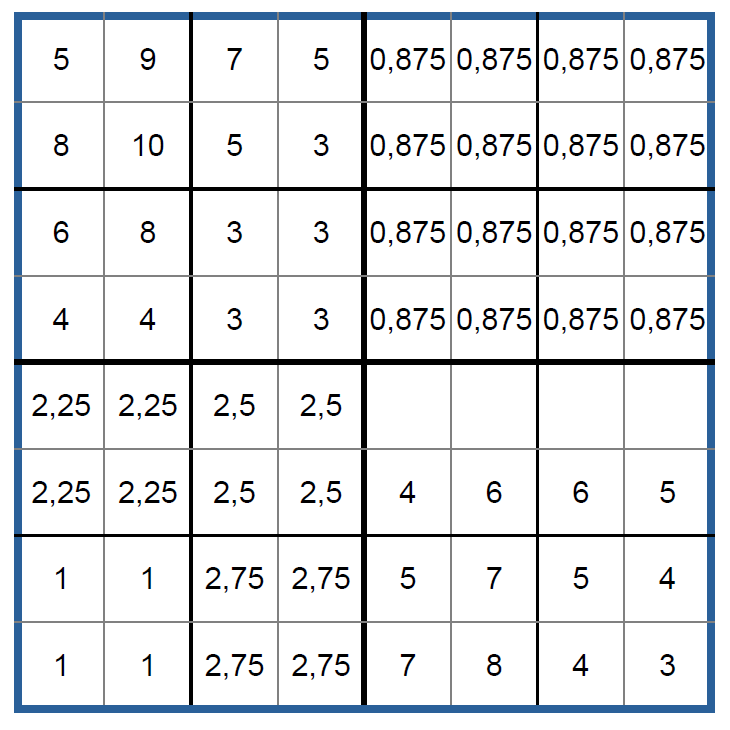
\includegraphics[width=\linewidth]{figures/Quadtree/adaptation_example_variante_sdcspatial_fix.png}
    %\vspace{-0.5cm}
    \caption{Result of \texttt{sdcSpatial} if applied on the grid of the example displayed in Fig.\ref{fig:quadtree_aggregation}.}
    \label{fig:quadtree_sdcspatial_result}
    % \end{figure}
\end{minipage}
\end{figure}




\subsection{A variant of the quadtree approach developped at Insee}\label{sec:variante_insee}


Insee has developed a method based on the quadtree to disseminate data from tax sources on a grid of $1$~km cells and another grid of $200$~m cells \citep{Branchu_Costemalle_Fontaine_2018}. This method has been implemented in the R package called \texttt{gridy} \citep{gridy}. 

The peculiarity of this dissemination is that the counts (population and number of households) are not confidential, but their breakdowns (by sex, by age, etc.) or the sum of individual incomes, the number of households living below the poverty line, etc. are subject to confidentiality rules. The method is also used by Insee for disseminating Census 2021 data on $1$~km cells. The confidentiality rule applied here is to not disseminate original information (other than the count) on cells containing fewer than $11$ households.

\subsubsection{How does it work?}

The quadtree is used in a top-down approach: the aggregation process starts from the minimal resolution level, i.e., the one at which no cell is below the threshold.

The idea is to gather risky tiles with other ones (and also with some non-risky tiles) so as to ensure that each group contains more households than the required threshold. The process begins from the coarsest level ($64$~km) and continues to the finest one ($200$~m). The groups are inherited from one level to the next, as shown in Figure~\ref{fig:multilayer_grid}. The top-down approach lets one refine the composition of the groups to avoid the aggregation of more cells than needed for the protection. At the end of the quadtree process, we get either original cells at the desired resolution ($1$~km for example) or groups of suppressed cells.

In fact, the suppression process is just temporary. Attribute counts at the group level are distributed among the cells on a \textit{pro rata} basis of the cell's population share in the group's population. The population of the cell, which is non-confidential information, thus serves as the key for distributing other attributes.

Consider a group of cells in which we wish to proceed with the imputation of the number of males and females in each of its cells.

Let the notations be:
   \begin{itemize}
    \item $P^c$, $P^c_f$, $P^c_m$, respectively, the total population, the number of women, and men actually living in the cell $c$;
    \item $\hat{p}^c$, $\hat{p}^c_f$, $\hat{p}^c_m$, their disseminated equivalents (after allocating);
    \item $P^g$, $P^g_f$, $P^g_m$, their equivalents at the level of group $g$.
\end{itemize}

The allocation principle consists of disseminating the following values:

\begin{equation}
\begin{split}
    \hat{p}^c_m &= P^g_m \cdot \frac{P^c}{P^g} \\
    \hat{p}^c_f &= P^g_f \cdot \frac{P^c}{P^g}    
\end{split}    
\end{equation}

Thus, the total population of cell $c$ after proportional allocation is indeed equal to the original population:

\begin{equation}
    \hat{p}^c = \hat{p}^c_f + \hat{p}^c_m = \frac{P^c}{P^g} \cdot (P^g_f + P^g_m) 
    = \frac{P^c}{P^g} \cdot P^g 
    = P^c
\end{equation}

\begin{figure}[H]
    \centering
    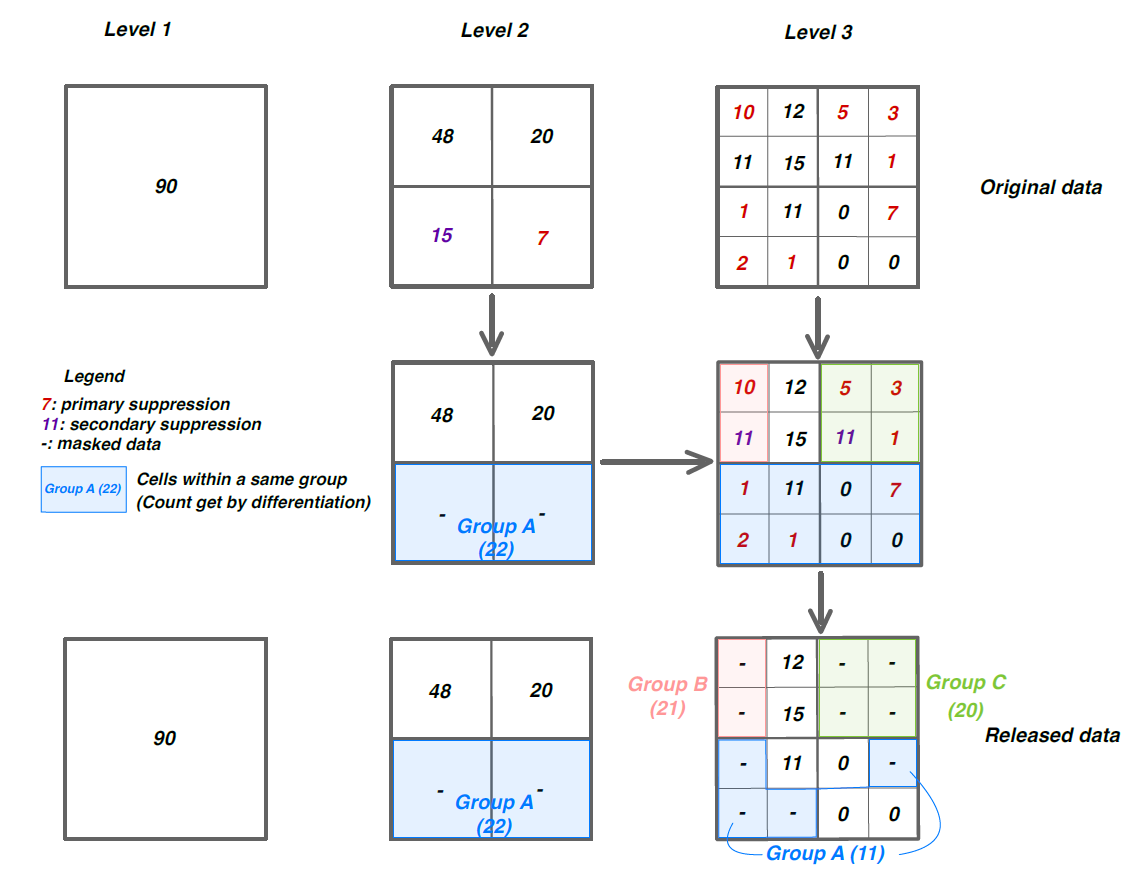
\includegraphics[width=\textwidth]{figures/Quadtree/grille_creu_proc_all.png}
    \caption{Building groups of risky tiles along a quadtree decomposition}
    \label{fig:multilayer_grid}
\end{figure}

\subsubsection{Risk and Utility aspects}

The method allows for handling the risk of attribute disclosure, and it is entirely conceivable to also address the risk of disclosure by inference by assigning one of the groups formed during the quadtree process to cells that would be too homogeneous on a (sensitive) attribute.

Nevertheless, this method  requires a variable used as a distribution key. It could then be useful when counts (population or households, for example) are not considered confidential, as is the case for population enumeration in France.

As this method is not a full perturbative one, it doesn't ensure a full protection against geographic differencing. Hence, some techniques presented in the section~\ref{sec:risk_diff} have to be applied.
In France, $78$\% of the $200$~m cells and $52$\% of the $1$~km cells are below the confidentiality threshold. 

In terms of utility, the method is quite interesting compared to a standard quadtree (Tab.~\ref{tab:insee_hell_kwd}; for the measures used see section \ref{sec:util_DD}). Indeed, it avoids aggregations over large cells or the suppression of a large amount of information.

It also preserves spatial structures in the case of the French release of Census 2021 data on a $1$~km grid, as seen in Fig.\ref{fig:moran-depts}: the Moran's $\mathcal{I}$, which measures spatial autocorrelation in data (see section \ref{sec:util_moran}), has not been significantly altered in most cases, when considering the French department level (the points of the plots) for the four attributes (one of the four plots).

\begin{table}[H]
\footnotesize
\caption{Utility assessment for some attributes ($1$~km cells)}\label{tab:insee_hell_kwd} 
\centering
\begin{tabular}[t]{lrr}
\toprule
Attributes & Hellinger Distance & Kantorovich-Wasserstein distance \\
\midrule
Males & 0.015 & 0.00484 \\
Over 65 yo & 0.062 & 0.02067 \\
Born in EU (except France) & 0.104 & 0.03862 \\
Residing abroad the year before & 0.117 & 0.05983\\
\bottomrule
\end{tabular}
\end{table}


\begin{figure}[H]
    \centering
    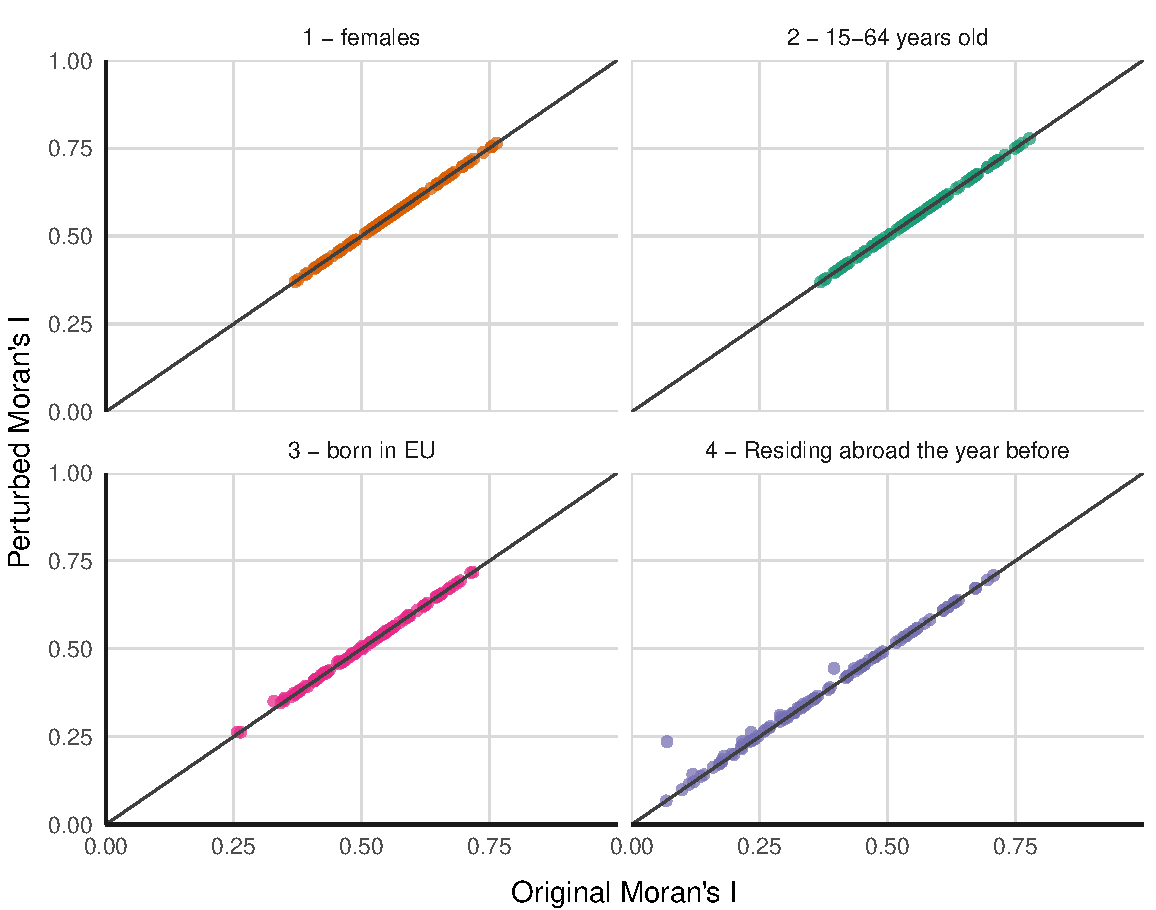
\includegraphics[width=\linewidth]{figures/Quadtree/carr_1km_moran_depts_4var_en_fix.pdf}
    \caption{Moran's $\mathcal{I}$ before and after treatment for several attributes, computed at the department level, departments being built from $1$~km tiles.}
    \label{fig:moran-depts}
\end{figure}

\newpage


    \section{Spatial Smoothing Method} \label{sec:methods_smooth}

Kernel smoothing, as described by \citep{Wand1994}, is a widely used method for
generating a smooth representation of measurements acquired at distinct points.
This approach bears resemblance to kernel density estimation
\citep{Silverman1986} and serves to highlight or reveal spatial patterns.
Consequently, an increasing number of publications adopt kernel smoothing to
visualize data originating from diverse sources such as road networks
\citep{Borruso2003}, crime statistics \citep{Chainey2002}, seismic damage
figures \citep{Danese2008}, and instances of diseases \citep{Davies2010}. 

In kernel density estimation, individual locations are diffused to create
density peaks surrounding each data point. These density peaks are then
aggregated and normalized to yield a comprehensive density. In the context of
kernel smoothing, however, no normalization is applied during the process. 

Kernel smoothing to protect data on a map has been described in e.g. \citet{JongeWolf2016}, \citet{DeWolfDeJonge2017}, \citet{WolfJonge2018} and \citet{Hut2020Thesis}. Kernel smoothing can be used as a spatial disclosure control method since it spatially blends observations: the value 
at a location on the map is the result of a spatial mixture of nearby observations. An attractive feature of using a kernel smoothing method is that it creates a smooth representation that both reveals spatial patterns as well as better protects individual observations. When using kernel smoothing for disclosure control, three distributions are essential: 
the spatial distribution of the population, the distribution of the variable that will be plotted and the ratio of the two. 
Spatial smoothing can be used to enforce $k$-anonymity and  ($n,k)$ dominance: areas with little observations may spatially blend with neighboring areas with many observations. 


Depending on the country context the spatial population density itself may not be considered sensitive; 
for example, some countries have public geospatial registers with buildings or publish 
population counts for the 100m $\times$ 100m grid. For those
countries the number of buildings or number of residents are 
not considered sensitive, but the plotted variable, e.g. unemployment rate or income can be sensitive.
The spatial distribution of such a sensitive 
variable for the population however must be checked for statistical disclosure. 
Whenever the population density is small, the sensitive variable runs the risk of 
being disclosed.

The kernel smoothed population density is given by 
\[ f_h(\vec{r}) = \frac{1}{h^2} \sum_{i=1}^N k\left(\frac{\vec{r}-\vec{r}_i}{h}\right)  , \]
in which $k\colon\mathbbm{R}^2\rightarrow\mathbbm{R}$ is a so-called \emph{kernel function}, that is, a non-negative, symmetric function that integrates to $1$ over $\mathbbm{R}^2$. The bandwidth $h$ controls the range of influence of each data point. 
Common choices are:
\begin{itemize}
    \item The Gaussian kernel $k(\vec{r}) = (1/2\pi) \exp(-||\,\vec{r}\,||^2/2)$,
    \item the Epanechnikov kernel $k(\vec{r}) = (2/\pi) (1-||\,\vec{r}\,||^2)\mathbbm{I}_{\{\vec{x}:||\,\vec{x}\,||\leq1\}}(\vec{r})$ and
    \item the uniform kernel $k(\vec{r}) = (1/\pi)\mathbbm{I}_{\{\vec{x}:||\,\vec{x}\,||\leq1\}}(\vec{r})$
\end{itemize} (with $\mathbbm{I}_S(y)=1$ if $y\in S$ and $\mathbbm{I}_S(y)=0$ if $y\notin S$ where $S$ is a given set). But obviously many others kernel functions exist. Some guidelines are given in Sect. 4.5 of \cite{Wand1994}.

For the measurements values $g_1,\ldots,g_N$, a density can be constructed by multiplying the kernel corresponding to location $i$ with the value $a_i$:
\[ g_h(\vec{r}) = \frac{1}{h^2} \sum_{i=1}^N a_i k\left(\frac{\vec{r}-\vec{r}_i}{h}\right)  . \]

By dividing the two densities $f_h$ and $g_h$, we get the Nadaraya-Watson kernel weighted average \citep{Watson1964}:
\begin{equation} \label{e:smooth}
m_h(\vec{r}) = \frac{g_h(\vec{r})}{f_h(\vec{r})} = \frac{\sum_{i=1}^N a_i k\left((\vec{r}-\vec{r}_i)/h\right)}{\sum_{i=1}^N k\left((\vec{r}-\vec{r}_i)/h\right)}, \quad \vec{r}\in\mathcal{D}.
\end{equation}
with $\mathcal{D}$ the spatial domain.

Whenever $f_h(\vec{r})=0$, it follows that $g_h(\vec{r})=0$ as well and in that case we define $m_h(\vec{r})=0$. This weighted average is an excellent tool for data visualisation and analysis \citep{Chacon2018}. The ratio $m_h(\vec{r}),\,r\in\mathcal{D}$ will be the function of which we will investigate disclosure properties and discuss a possible protection method.

Some remarks are in order. Firstly, the bandwidth $h$ influences the smoothness of $m_h$. In the limit case of a very large bandwidth, $m_h$ will be constant, while for small $h$, the plot will contain many local extrema. In the limit case of a very small bandwidth, $m_h$ will be the nearest neighbour interpolation, at least when using a Gaussian kernel. Secondly, note that mass can leak away at the boundaries of the map, i.e. the sum (or integral) over both $g_h(\vec{r})$ and $f_h(\vec{r})$ density may be less than the total population and the total sum of the variable respectively, since $\mathcal{D}$ is bounded but the kernel is defined on $\mathbbm{R}^2$, meaning that smoothing may move density outside the area of interest. Consequently, $f_h$ and $g_h$ underestimate the (weighted) population density at $\vec{r}$ close to the boundary of $\mathcal{D}$. Various techniques to correct such edge effects exist, see \citet{Berman1989,Diggle1985,Lieshout2012}.

\subsection{A visual example}

Figure \ref{fig:sm_density} displays a synthetic dataset of enterprises and 
their production in a region in the Netherlands. In this dataset the 
locations of enterprises are realistic, since the Netherlands has 
a public register of residential and commercial buildings. For each building
a fictitious production value has been sampled from a log-normal distribution
and they are resampled to include some spatial correlation. 

\begin{figure}[H]
    \centering
    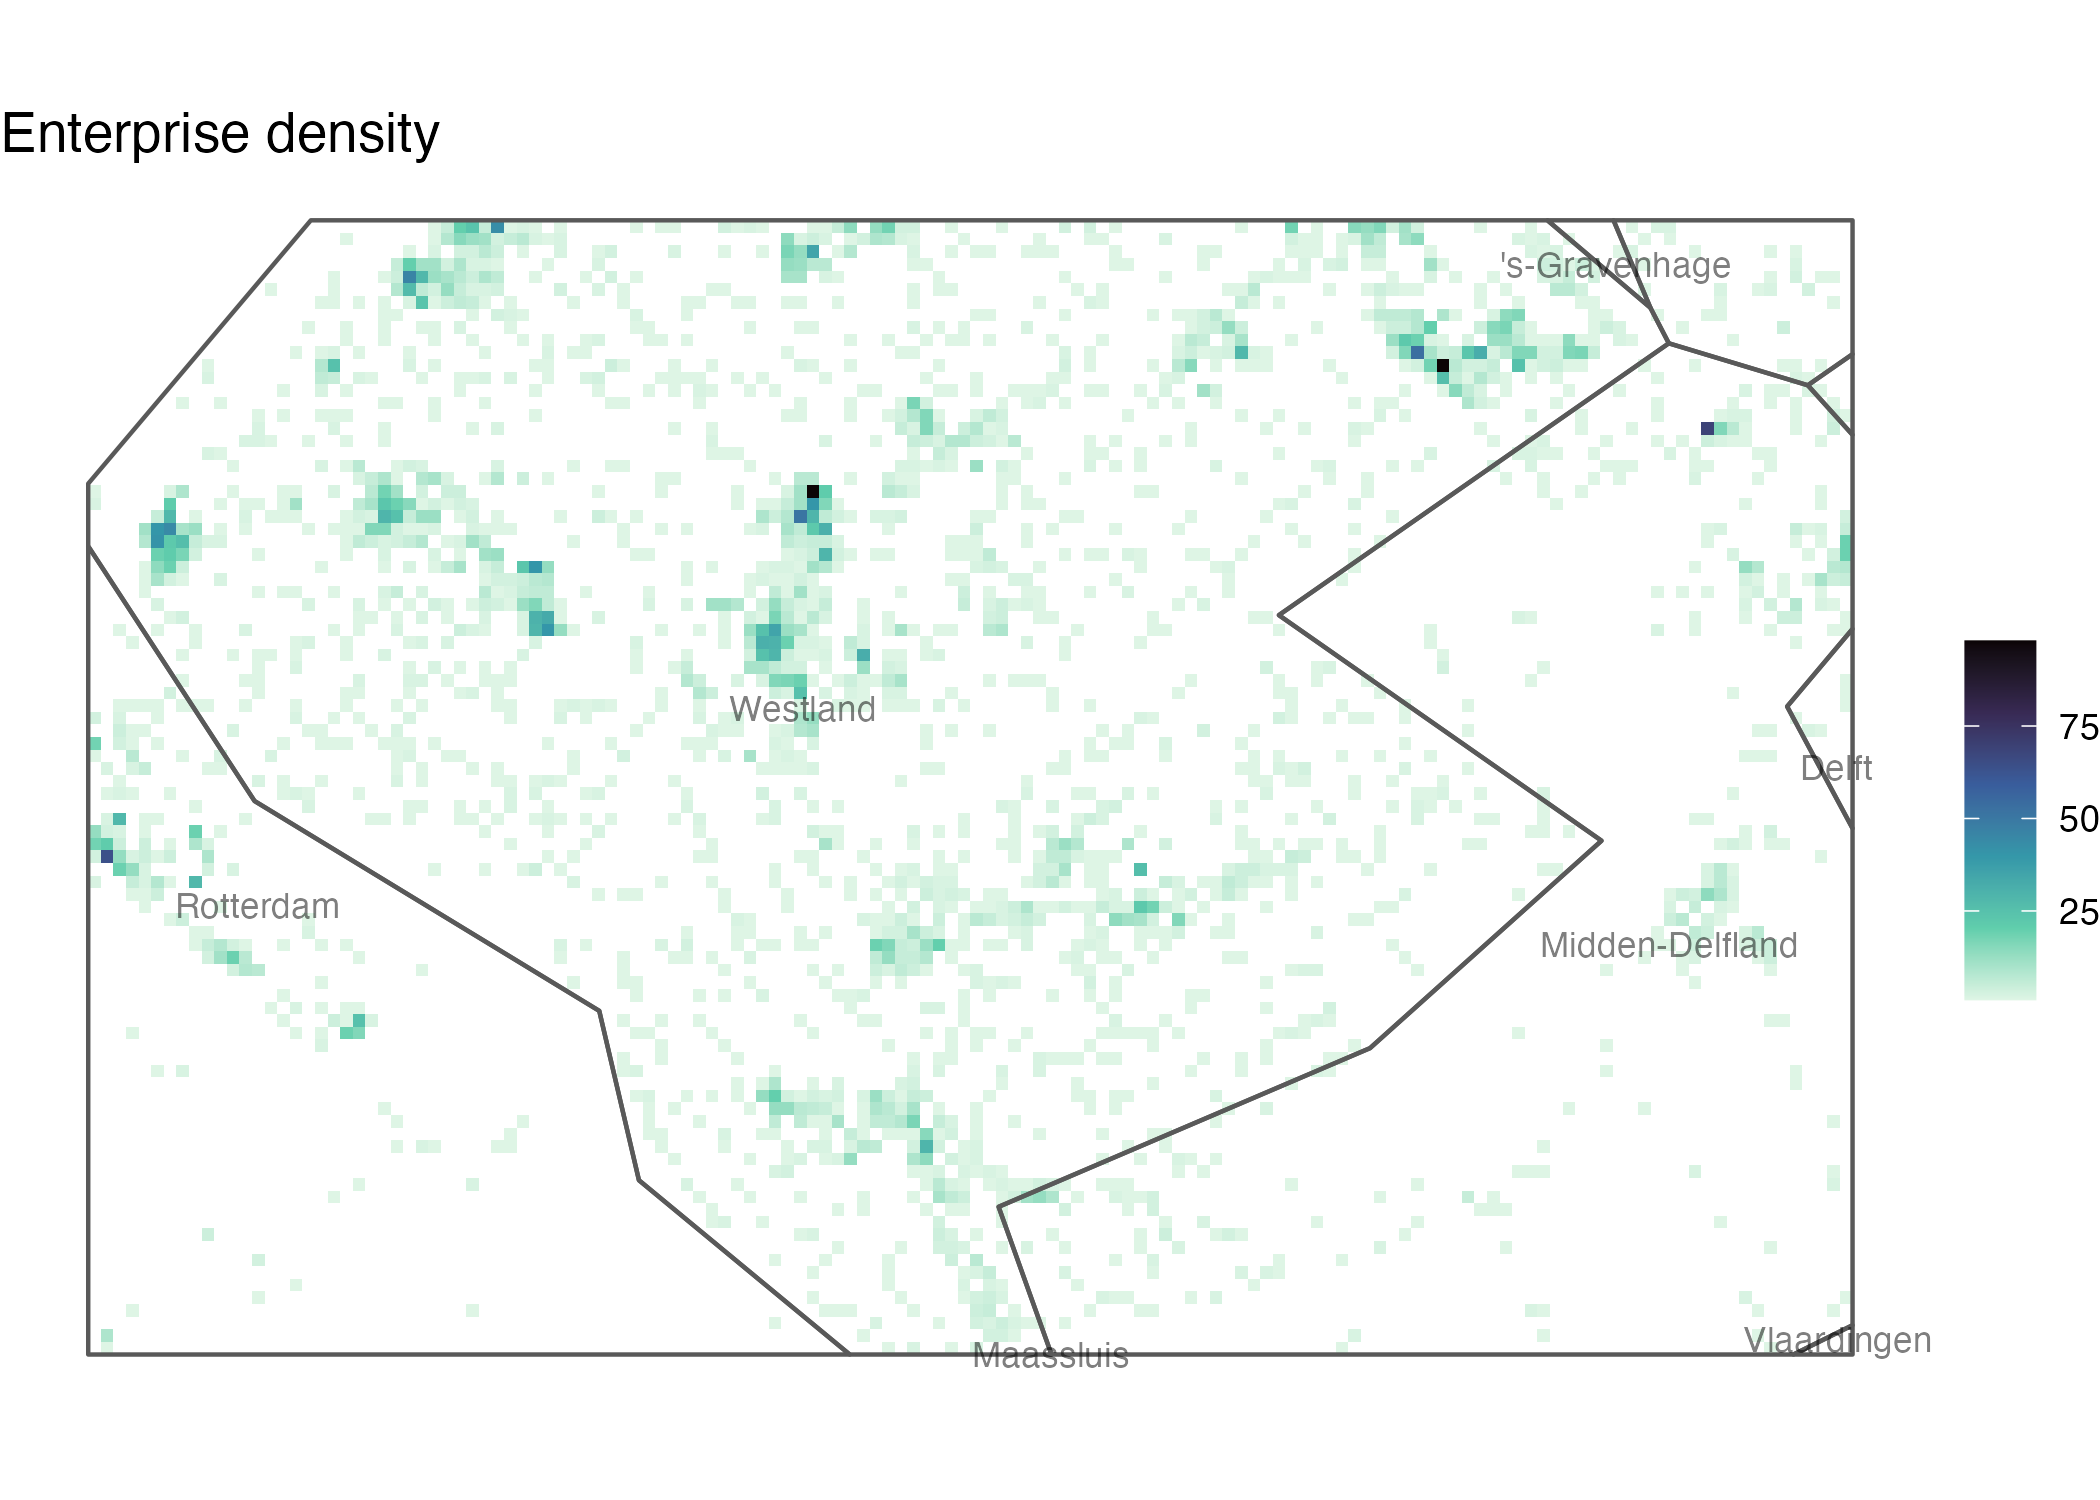
\includegraphics[width=.8\linewidth]{figures/Smoothing/enterprise_density.png} \\
    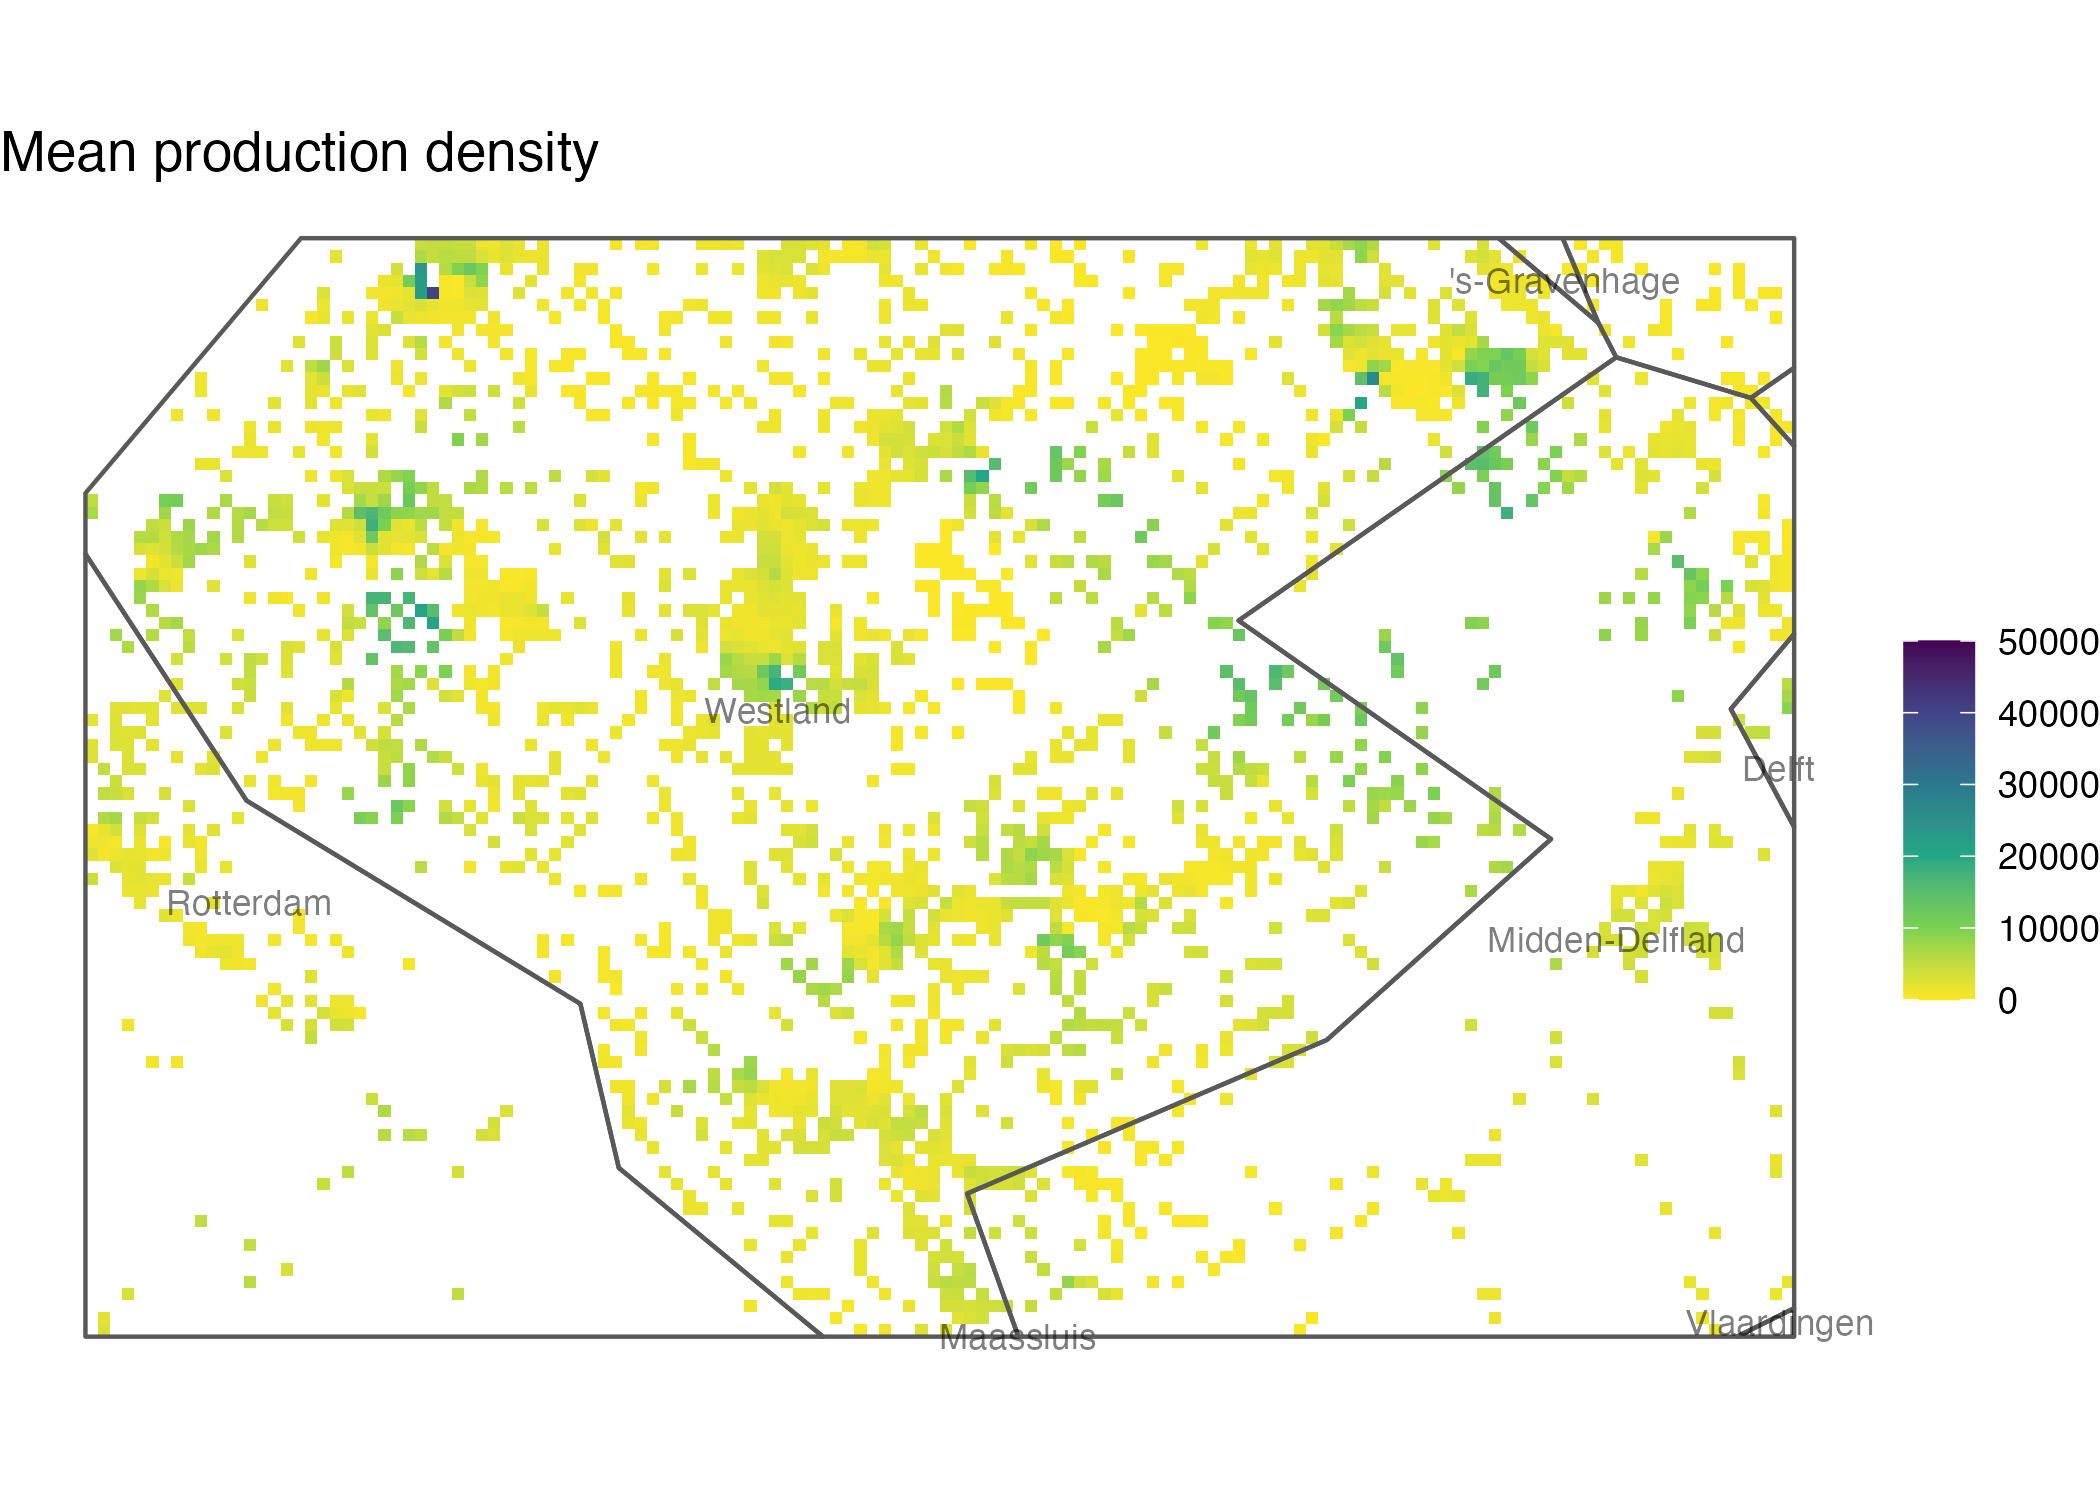
\includegraphics[width=.8\linewidth]{figures/Smoothing/mean_production_density.png}
    \caption{Density of enterprises (realistic) and their mean production (fictitious), created using \texttt{sdcSpatial} \citep{sdcSpatial_2022}}
    \label{fig:sm_density}
\end{figure}

Many geographical phenomena have
a skewed spatial distribution as figure \ref{fig:sm_density} exemplifies: enterprises and houses tend to cluster in 
geographical space. The enterprises are plotted in a 100m square grid, in which each grid cell contains the number of enterprises and the mean production within that grid cell. 

Common sense and figure \ref{fig:sm_sensitive} shows that most grid cells are unsafe for publication (in red), since most cells contain few enterprises: the cells of a 100m square grid are not expected to have high counts of enterprises.


\begin{figure}[H]
    \centering
    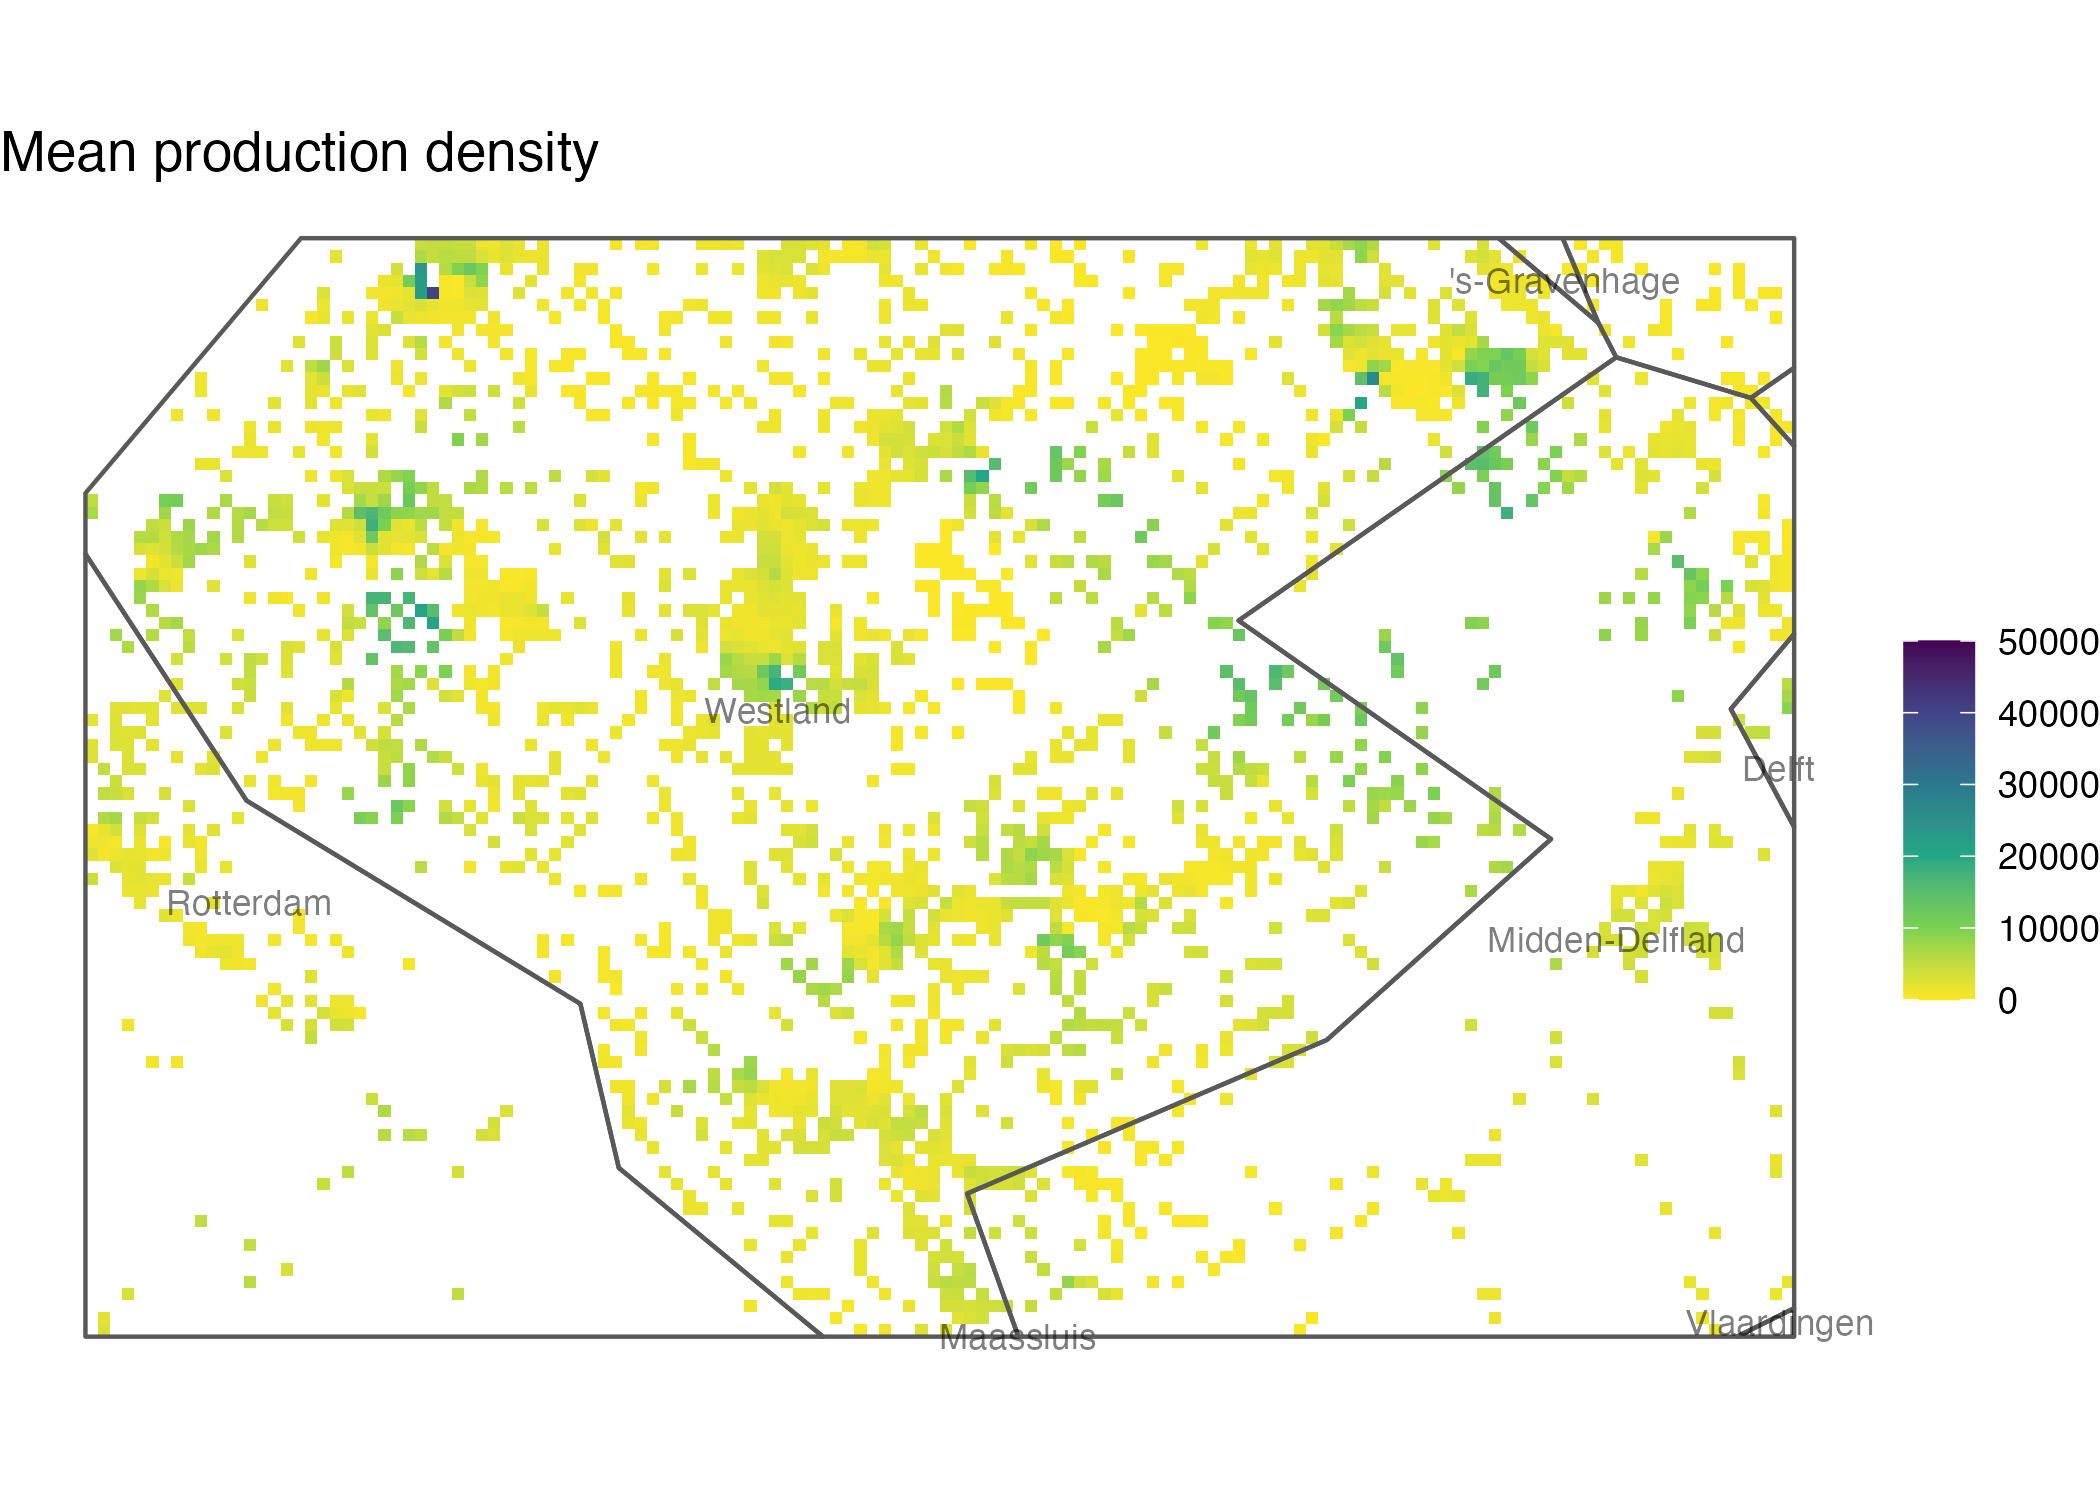
\includegraphics[width=.8\linewidth]{figures/Smoothing/mean_production_density.png} \\
    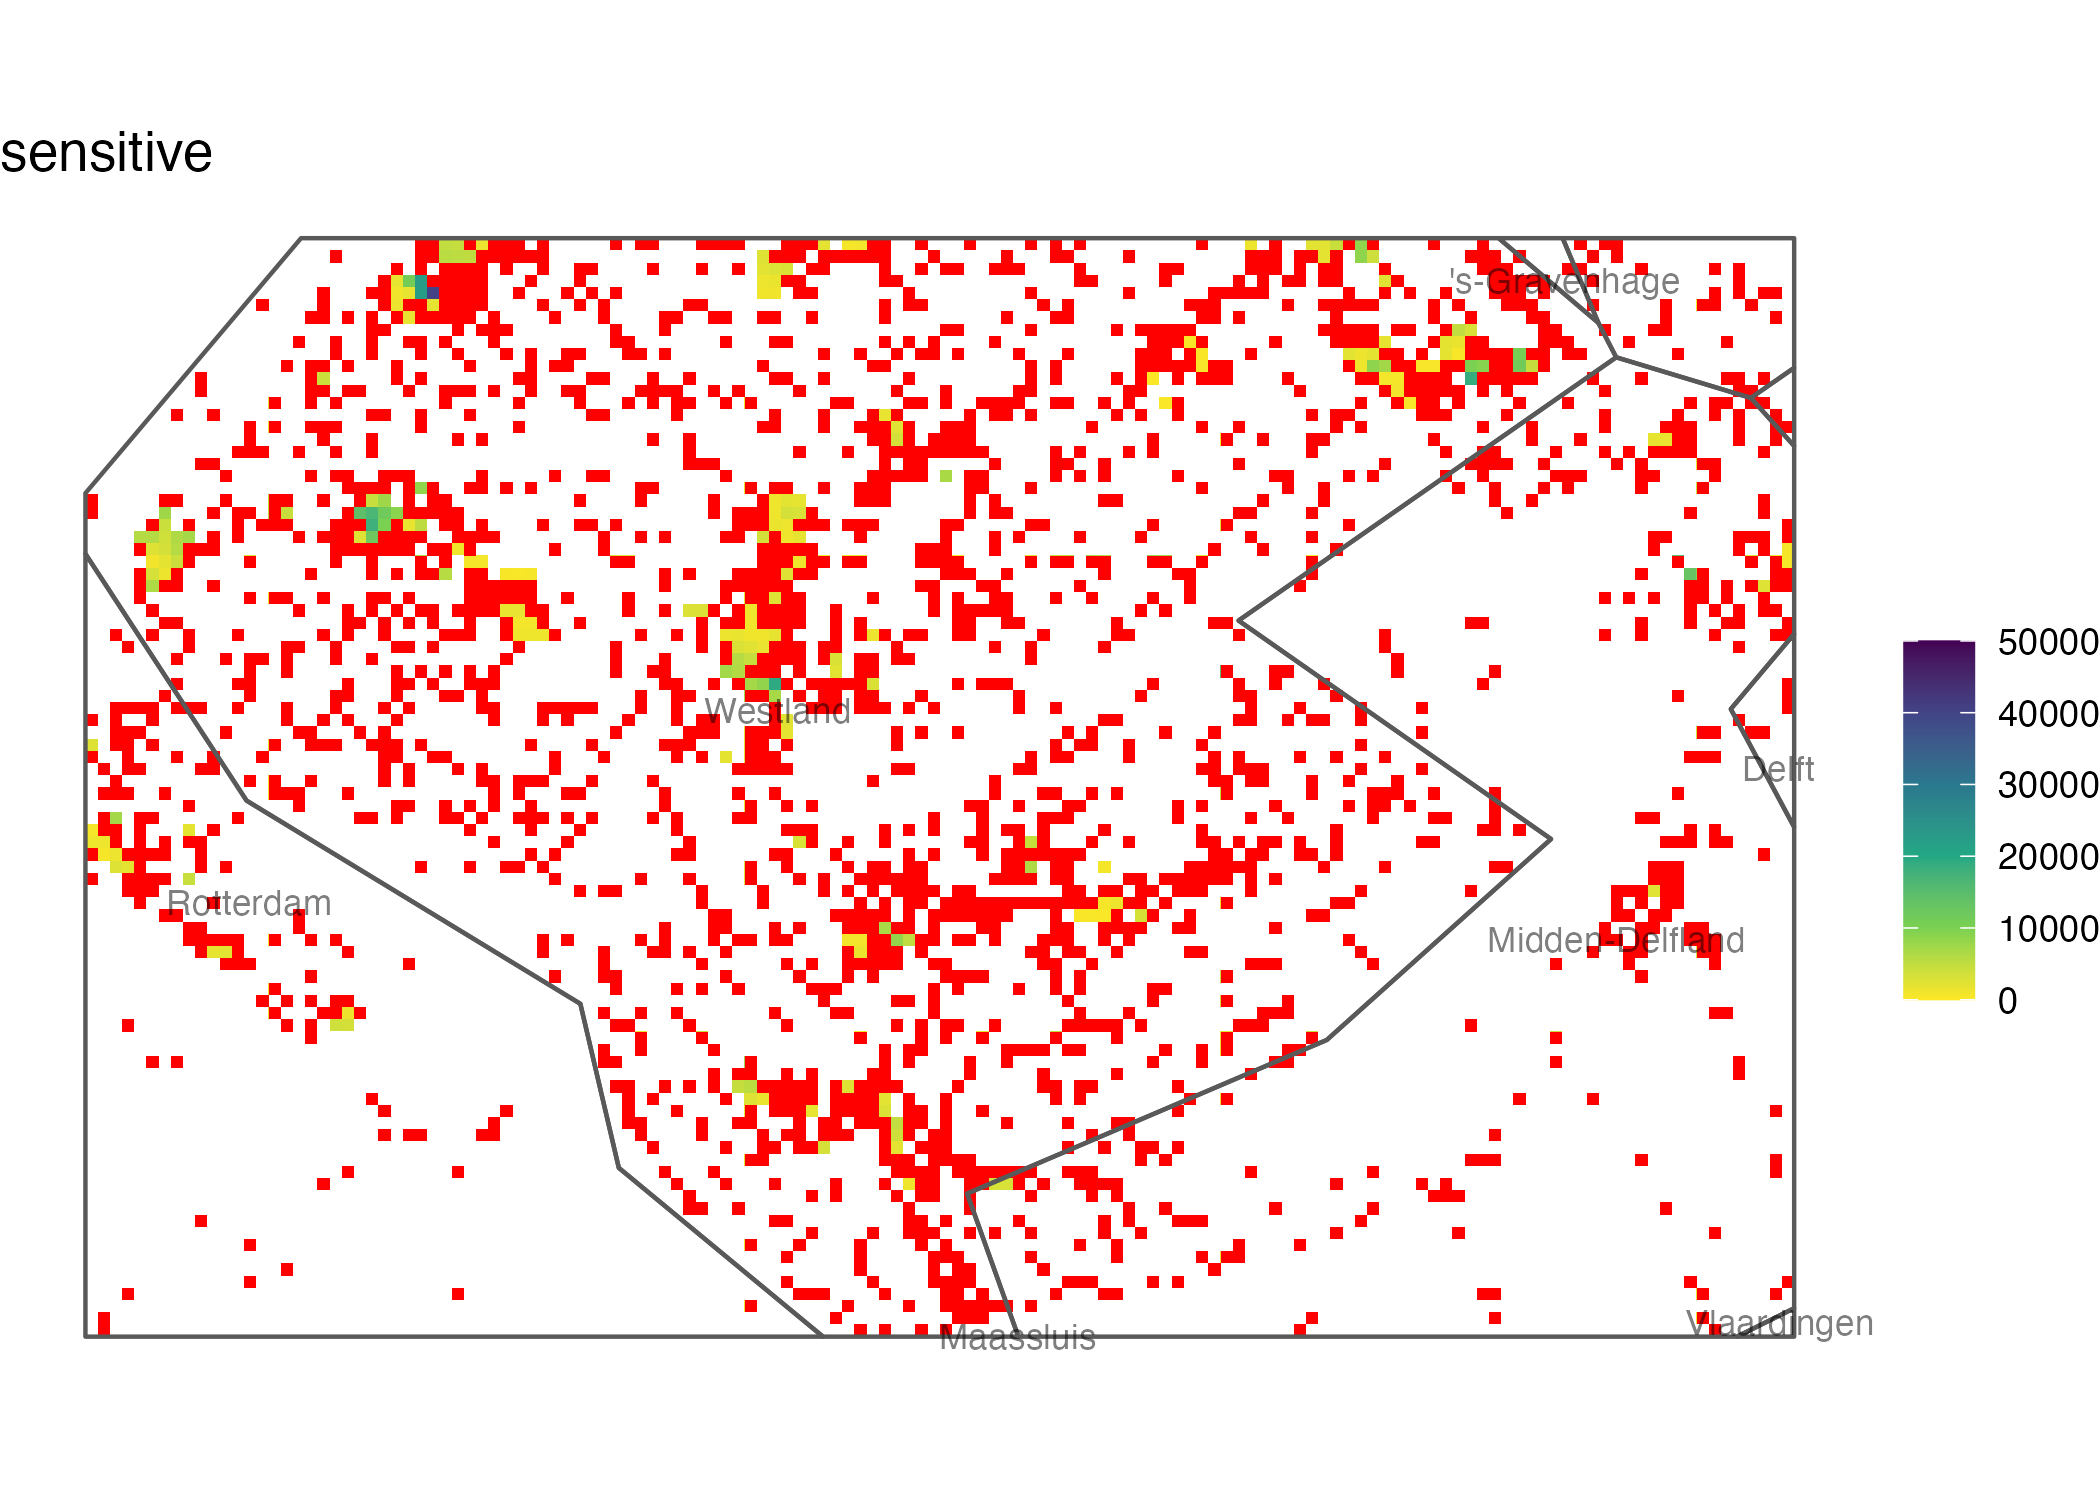
\includegraphics[width=.8\linewidth]{figures/Smoothing/sensitive.png}
    \caption{Mean production (left) and which grid cells are sensitive (right); most have too few enterprises to be safe.}
    \label{fig:sm_sensitive}
\end{figure}

\subsection{Spatial grid and resolution}

Equation (\ref{e:smooth}) is defined with $\vec{r}$ on $\mathbbm{R}^2$, 
but in practice a map is made discrete and published on a spatial grid
with a certain resolution. Furthermore, the computation of a spatial smoothing operation includes a spatial grid, e.g. it results in a dataset which has a fixed spatial resolution.

It is useful to define the risk function using a grid cell in the spatial grid. E.g. $k$-anonymity can easily be defined per grid cell as well as
$(n,k)$ dominance. 

A simple solution to reduce the disclosure risk is by coarsening the grid as 
is shown in figure \ref{fig:sm_resolution_dep}: plotting the data 
on increasingly coarser grids, i.e. with an increasing minimal resolution.

\begin{figure}[H]
    \centering
    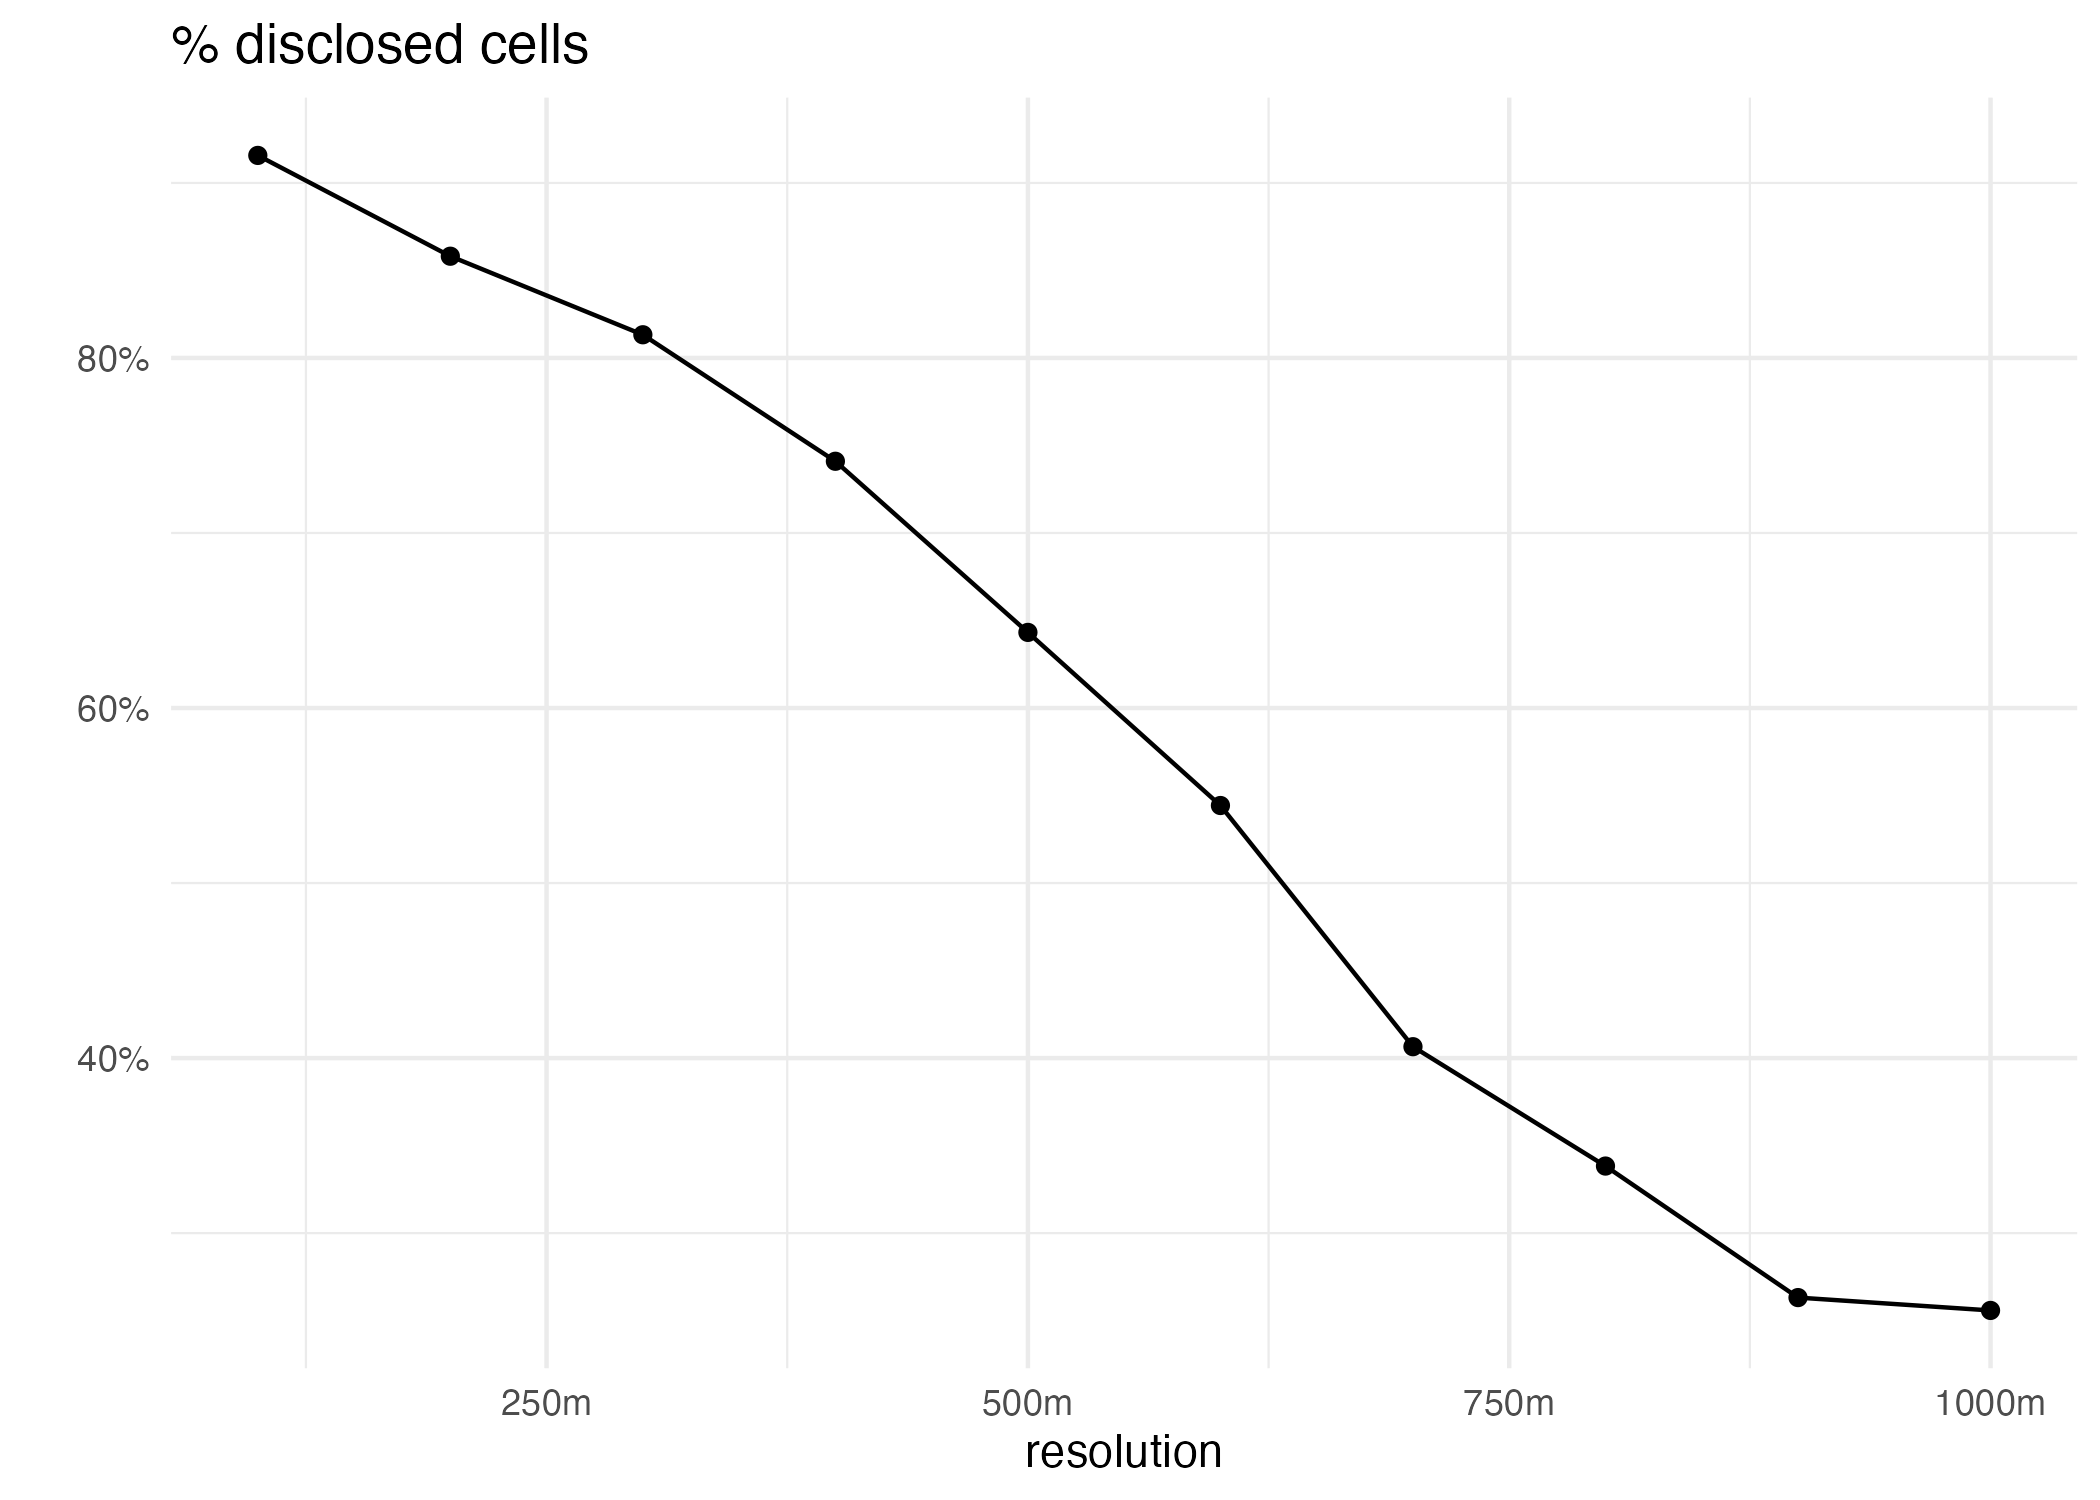
\includegraphics[width=.8\linewidth]{figures/Smoothing/sensitive_res.png}
    \caption{Disclosure risk for the dataset with increasing minimal resolution.}
    \label{fig:sm_resolution_dep}
\end{figure}

The risk-utility trade off can be seen in figure \ref{fig:sm_resolution}:
with increasing resolution, the resulting map becomes more blocky.

\begin{figure}[H]
    \centering
    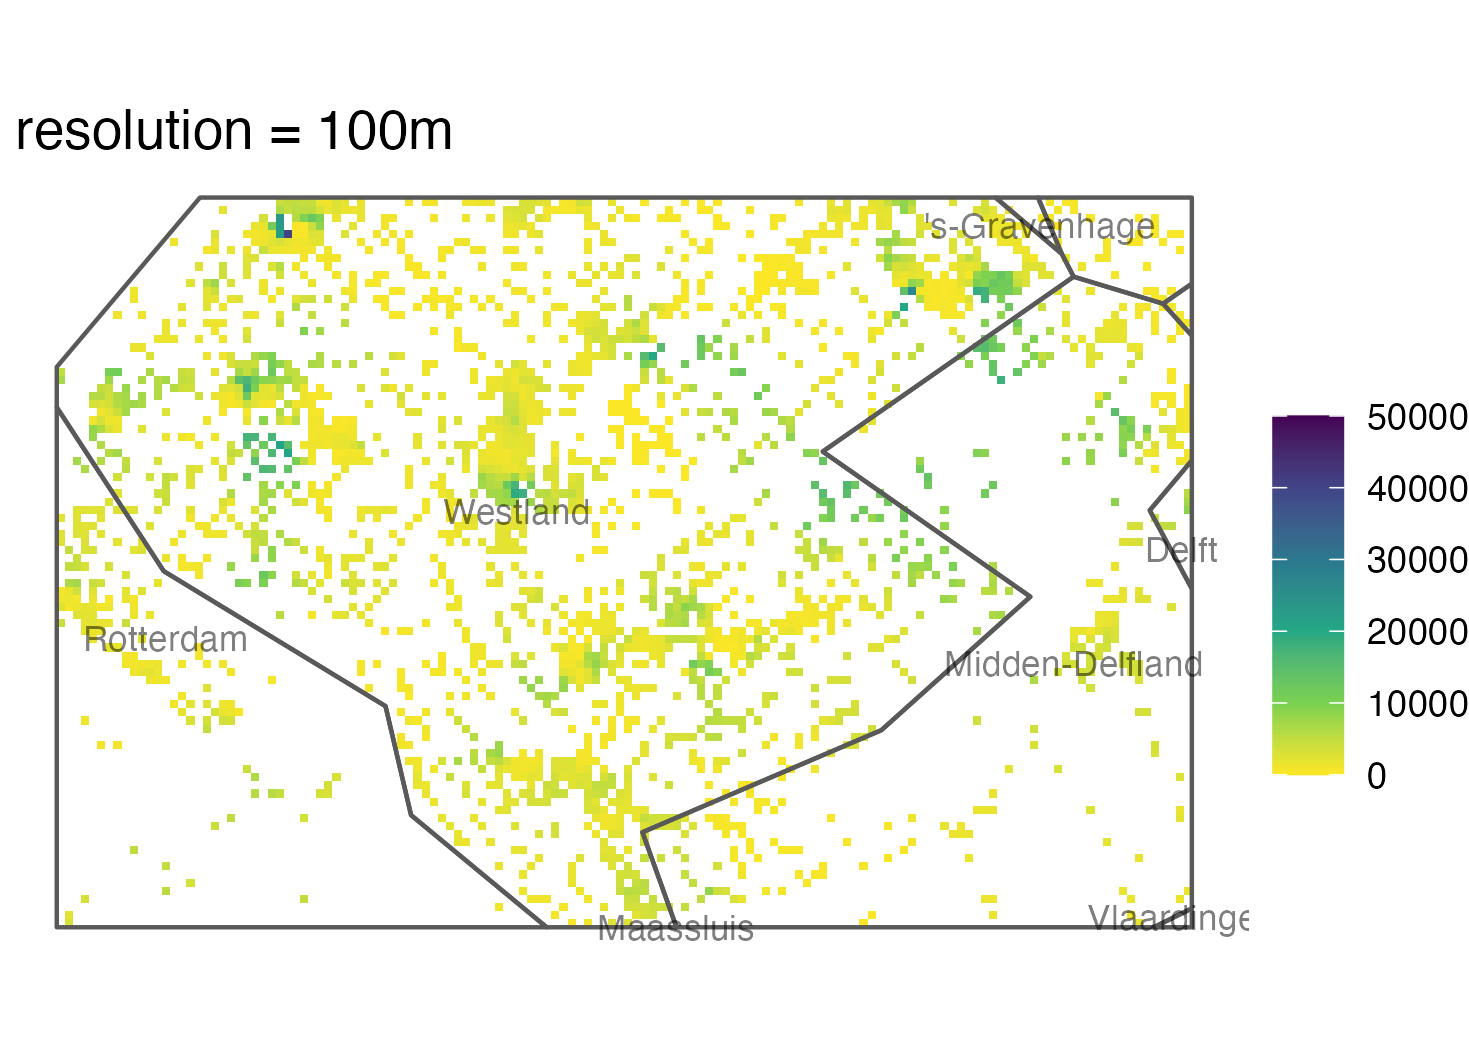
\includegraphics[width=.49\linewidth]{figures/Smoothing/res_100.png}
    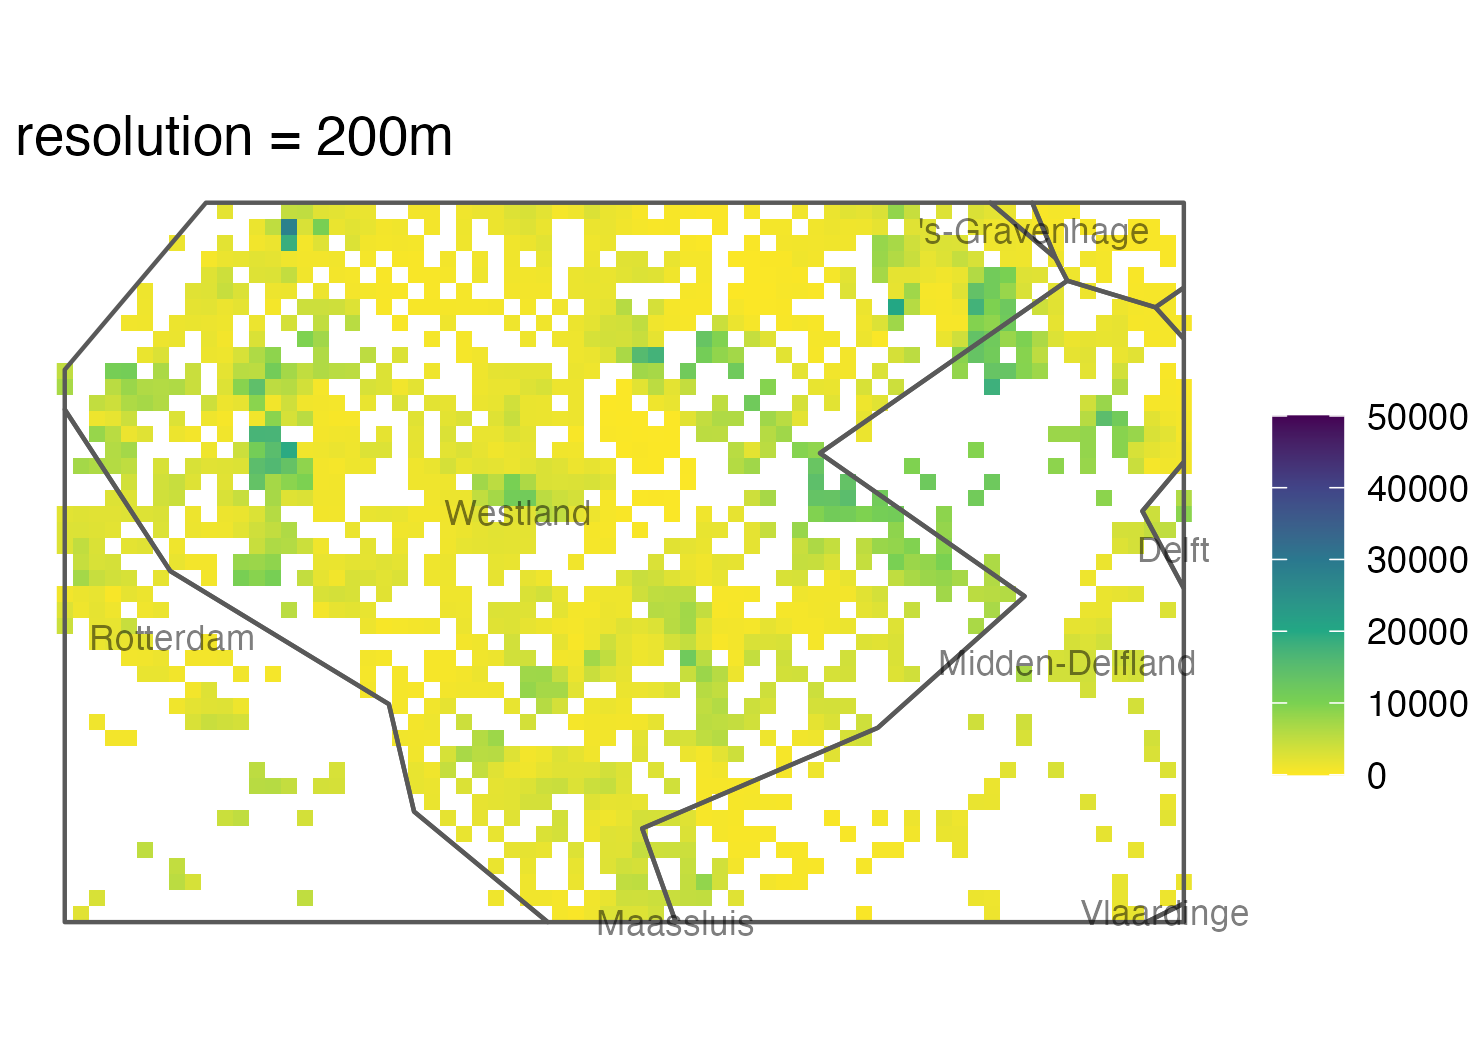
\includegraphics[width=.49\linewidth]{figures/Smoothing/res_200.png}\\
    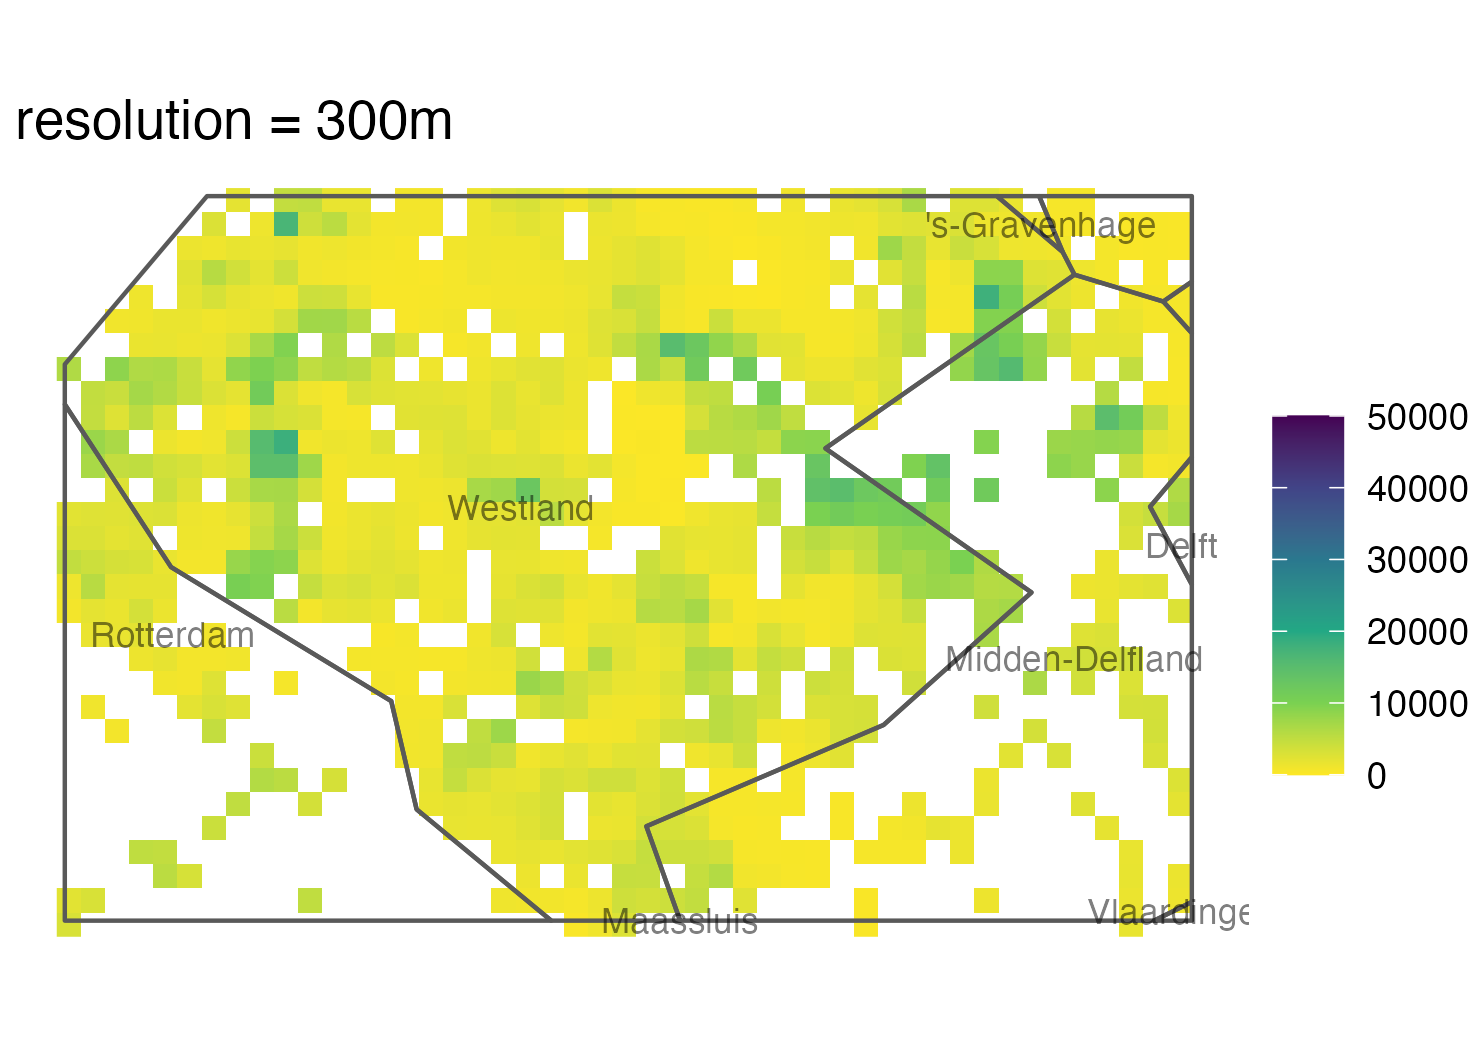
\includegraphics[width=.49\linewidth]{figures/Smoothing/res_300.png}
    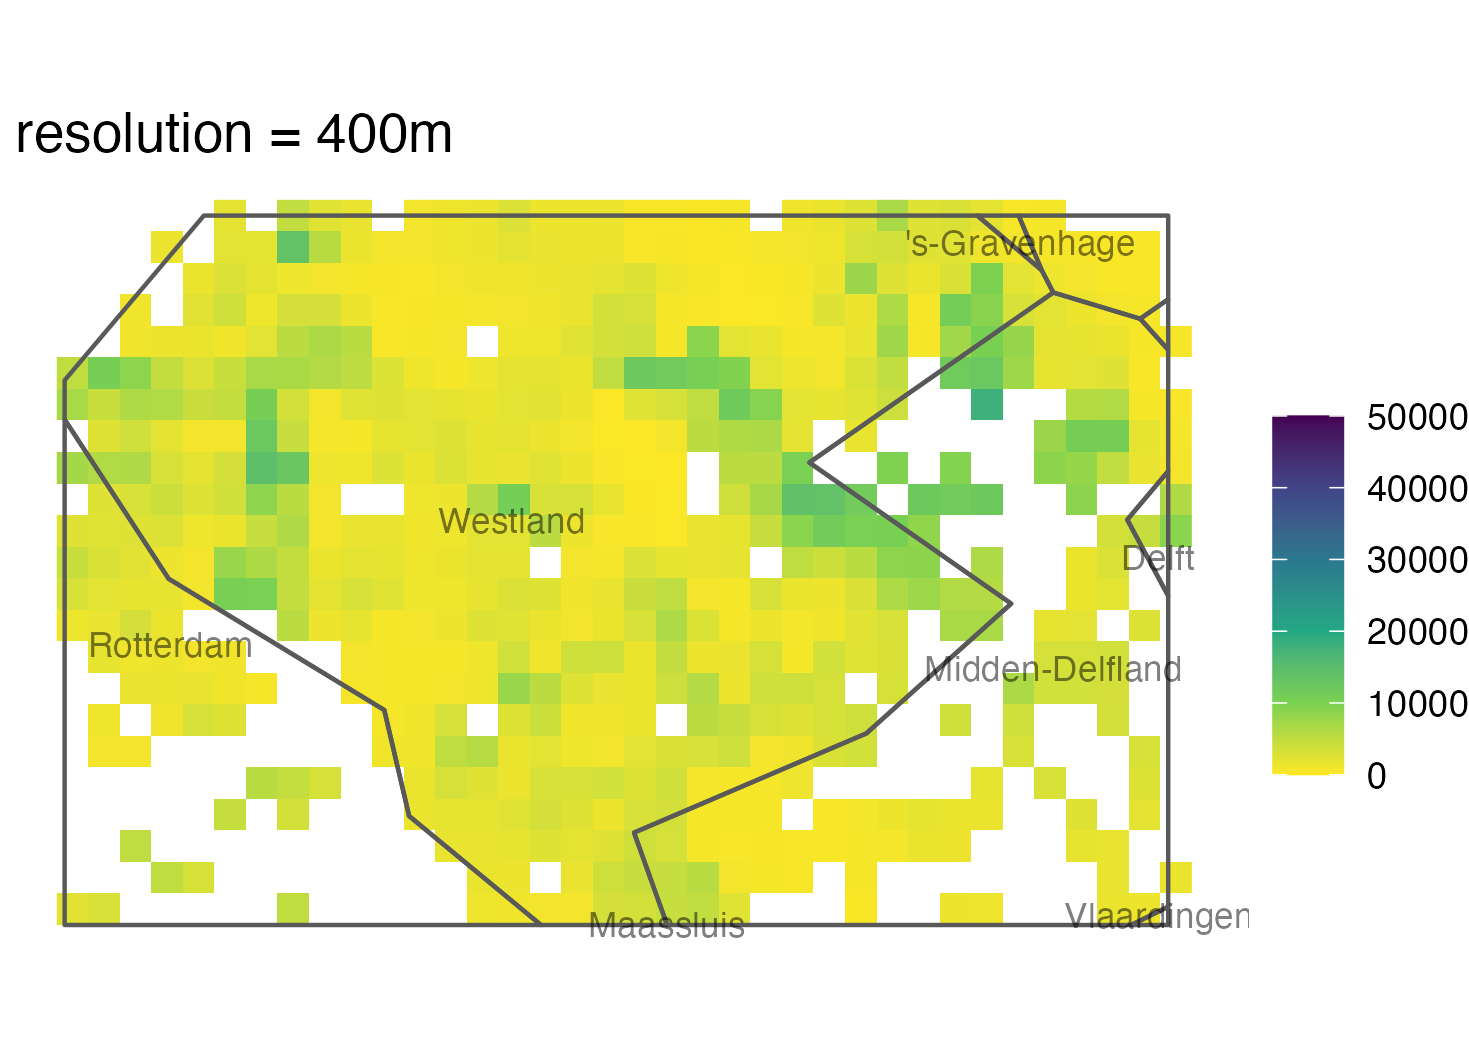
\includegraphics[width=.49\linewidth]{figures/Smoothing/res_400.png}\\
    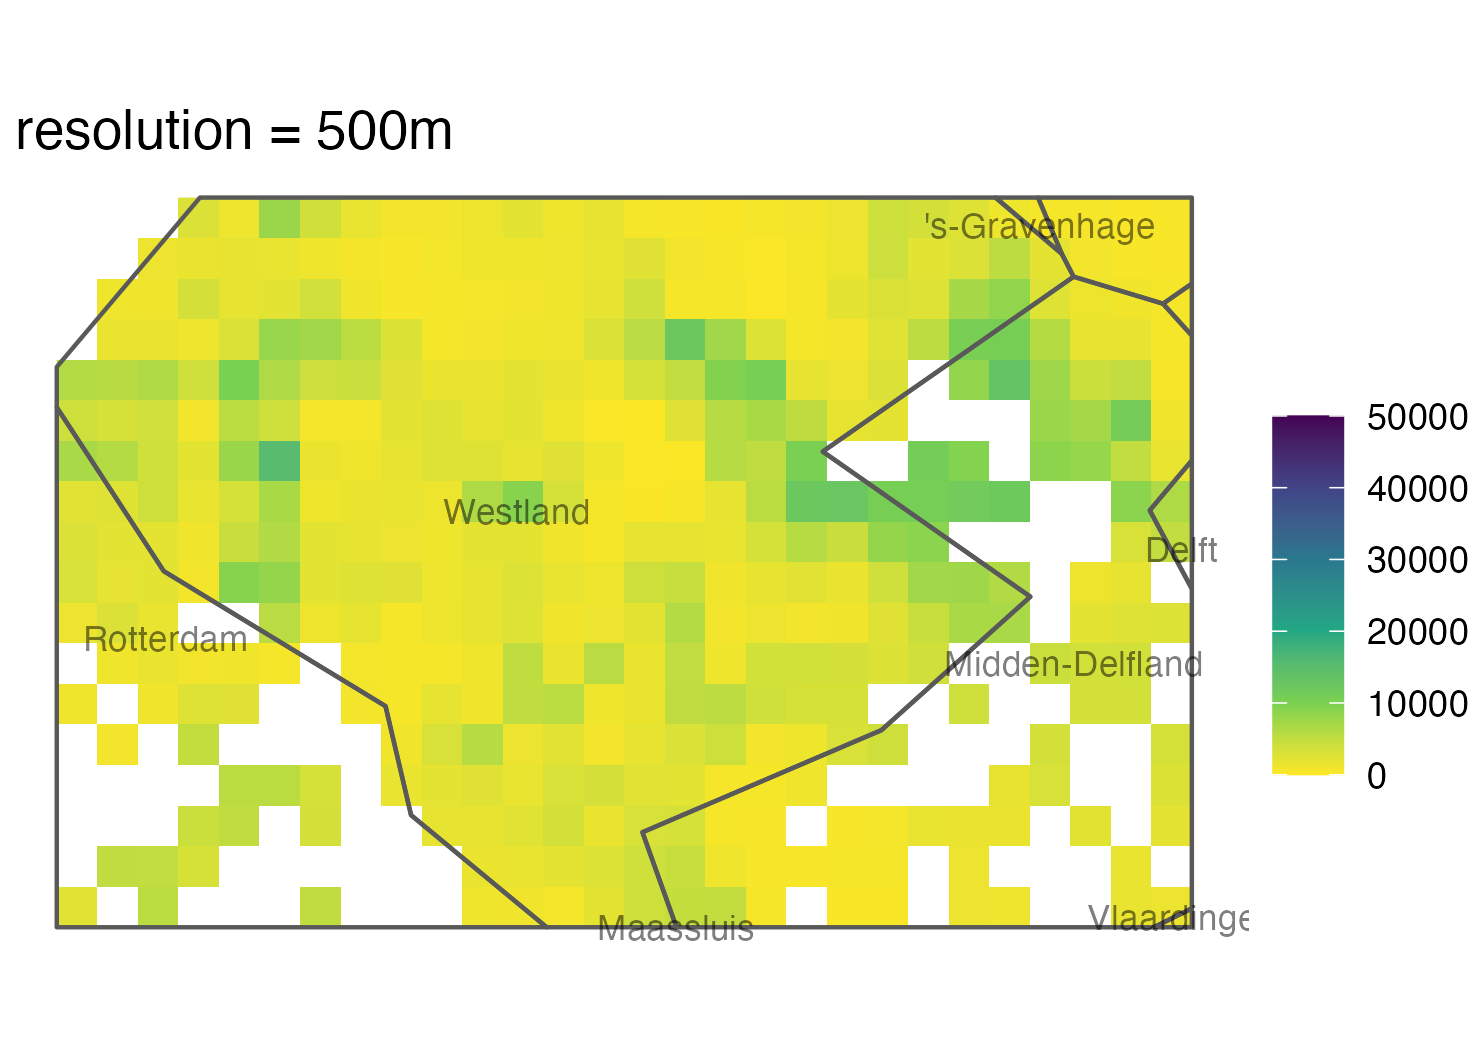
\includegraphics[width=.49\linewidth]{figures/Smoothing/res_500.png}
    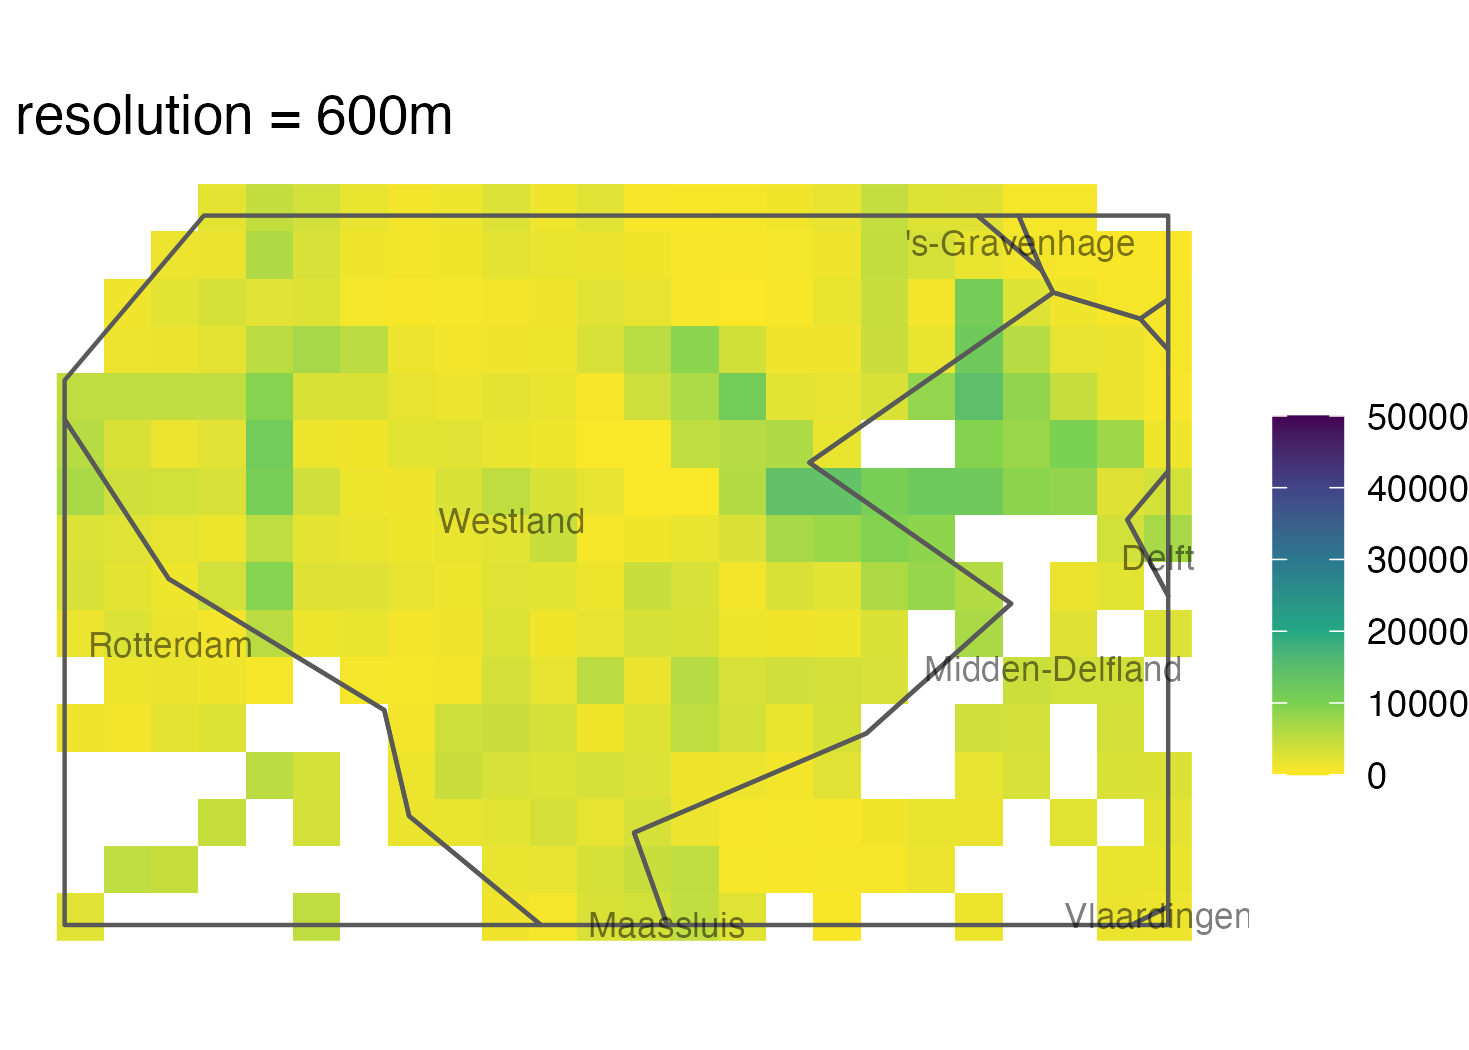
\includegraphics[width=.49\linewidth]{figures/Smoothing/res_600.png}\\
    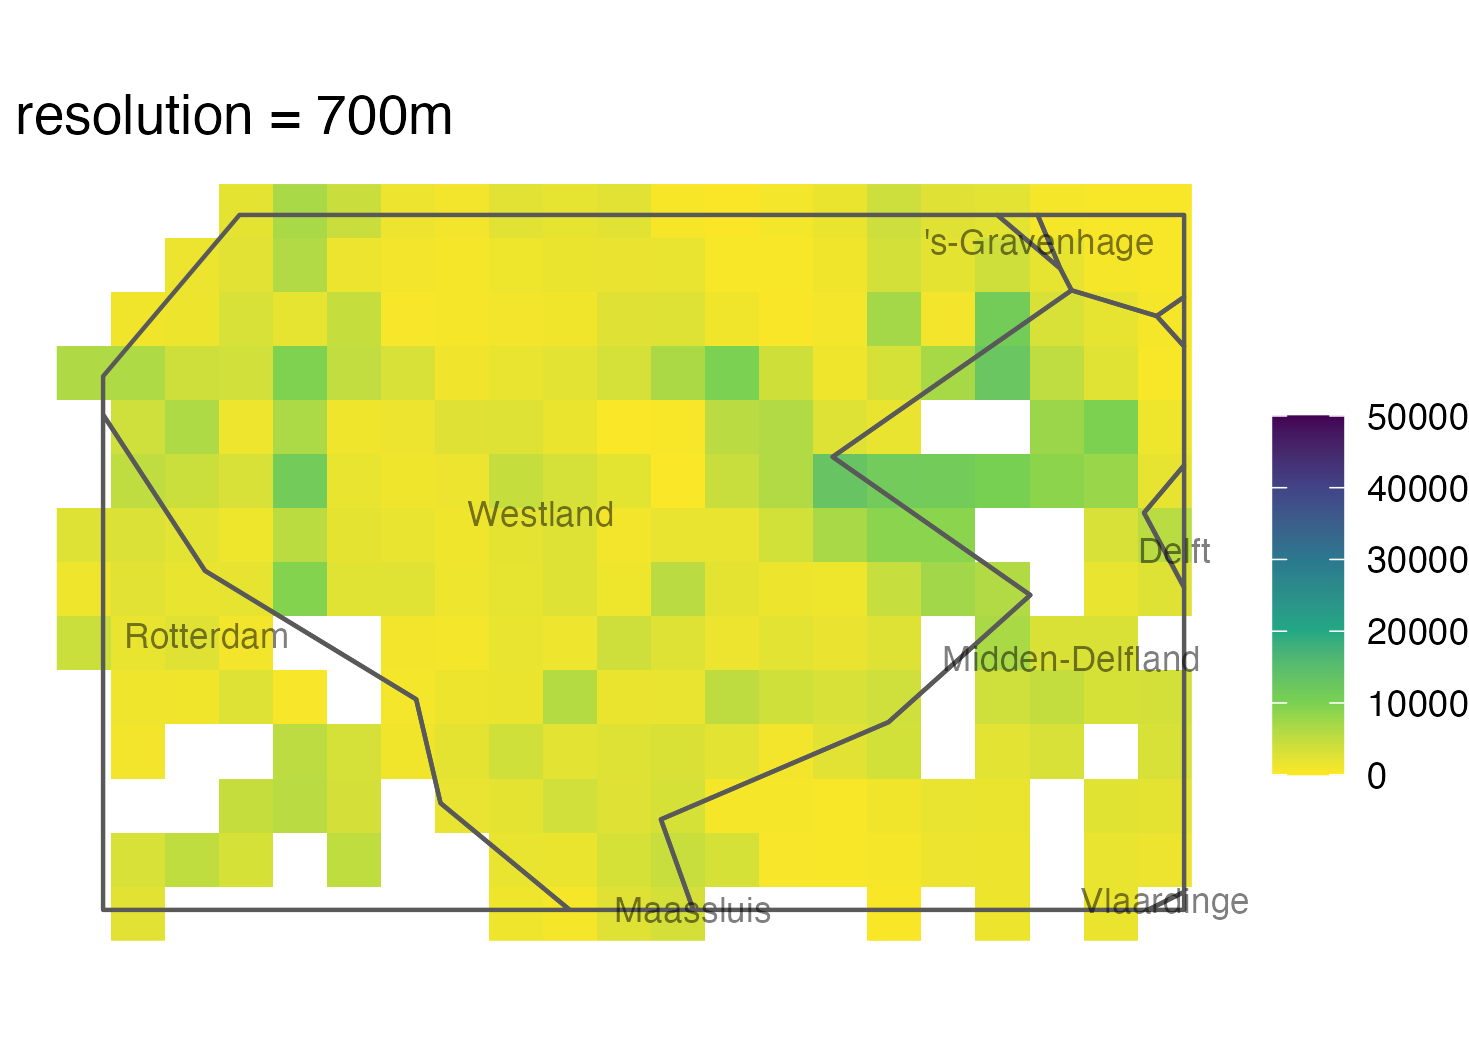
\includegraphics[width=.49\linewidth]{figures/Smoothing/res_700.png}
    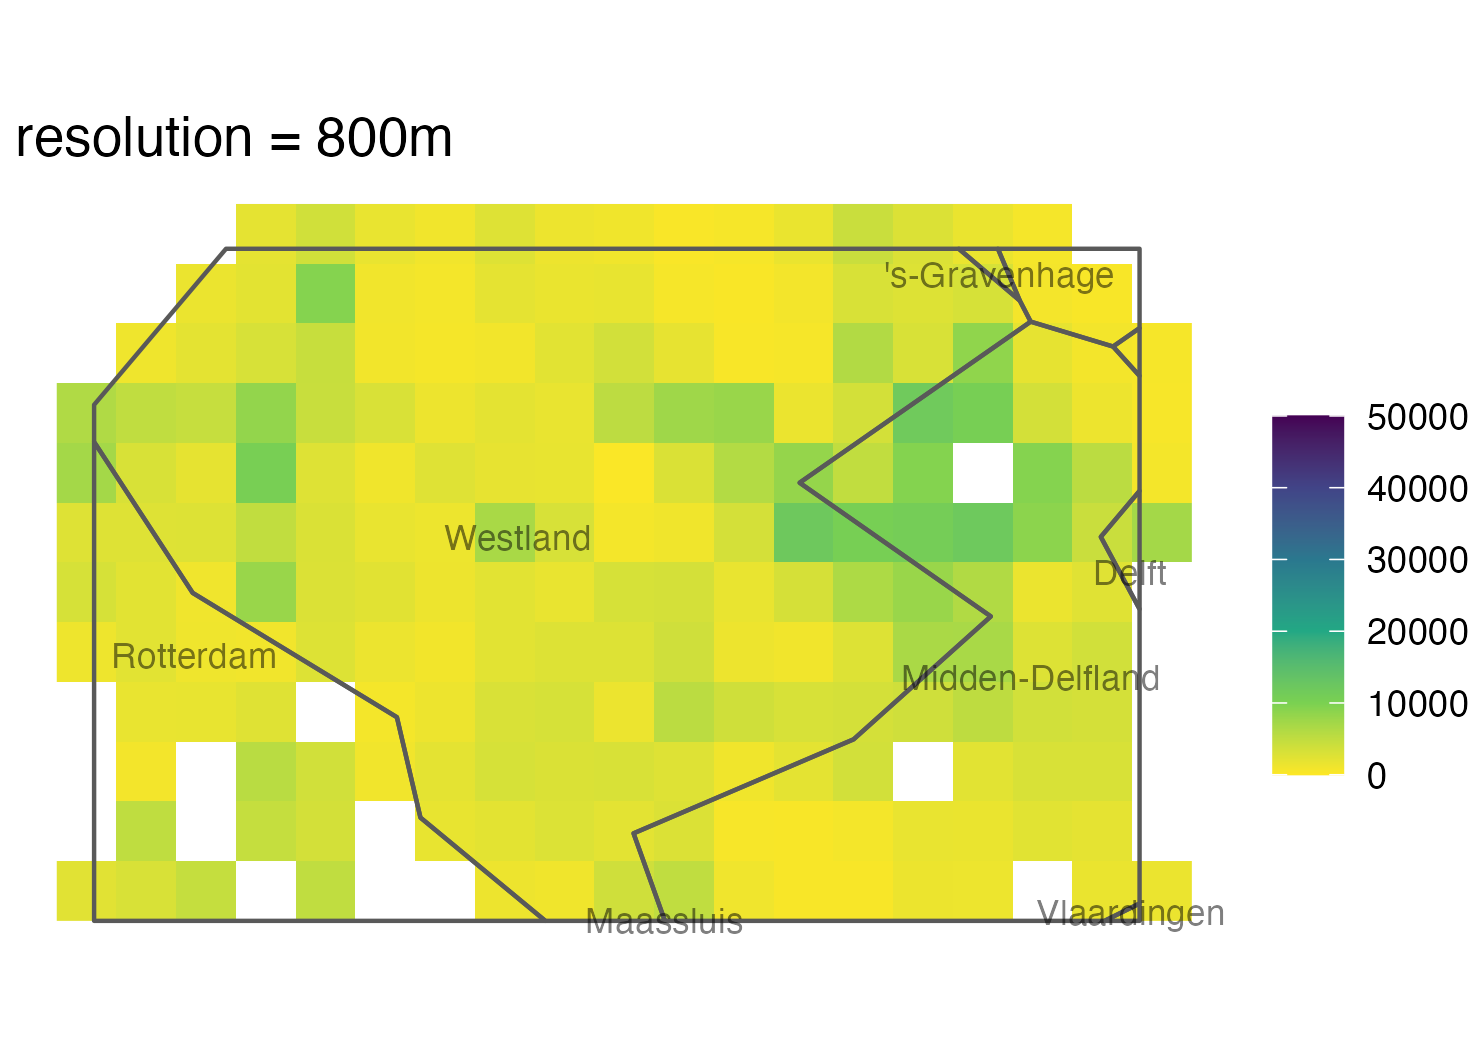
\includegraphics[width=.49\linewidth]{figures/Smoothing/res_800.png}\\
    \caption{Coarsening the grid by increasing the resolution (100-800m).}
    \label{fig:sm_resolution}
\end{figure}

Improving the utility of the map can be done by borrowing or blending values from 
neighboring cells: by smoothing using a Gaussian kernel smoother. 

\subsection{Risk and utility for band widths}

An other important parameter for kernel smoothing is the choice of the band width.
Increasing the band width reduces the number of unsafe locations and cells as
can be seen in figure \ref{fig:sm_sensitive_bw} where kernel smoothing is 
applied to the synthetic dataset. As sensitivity score, the $k$-anonymity with $k = 10$ is taken. When applying a smoothing operation on a spatial grid, the $k$-anonymity risk boundary is also smoothed.

\begin{figure}[H]
    \centering
    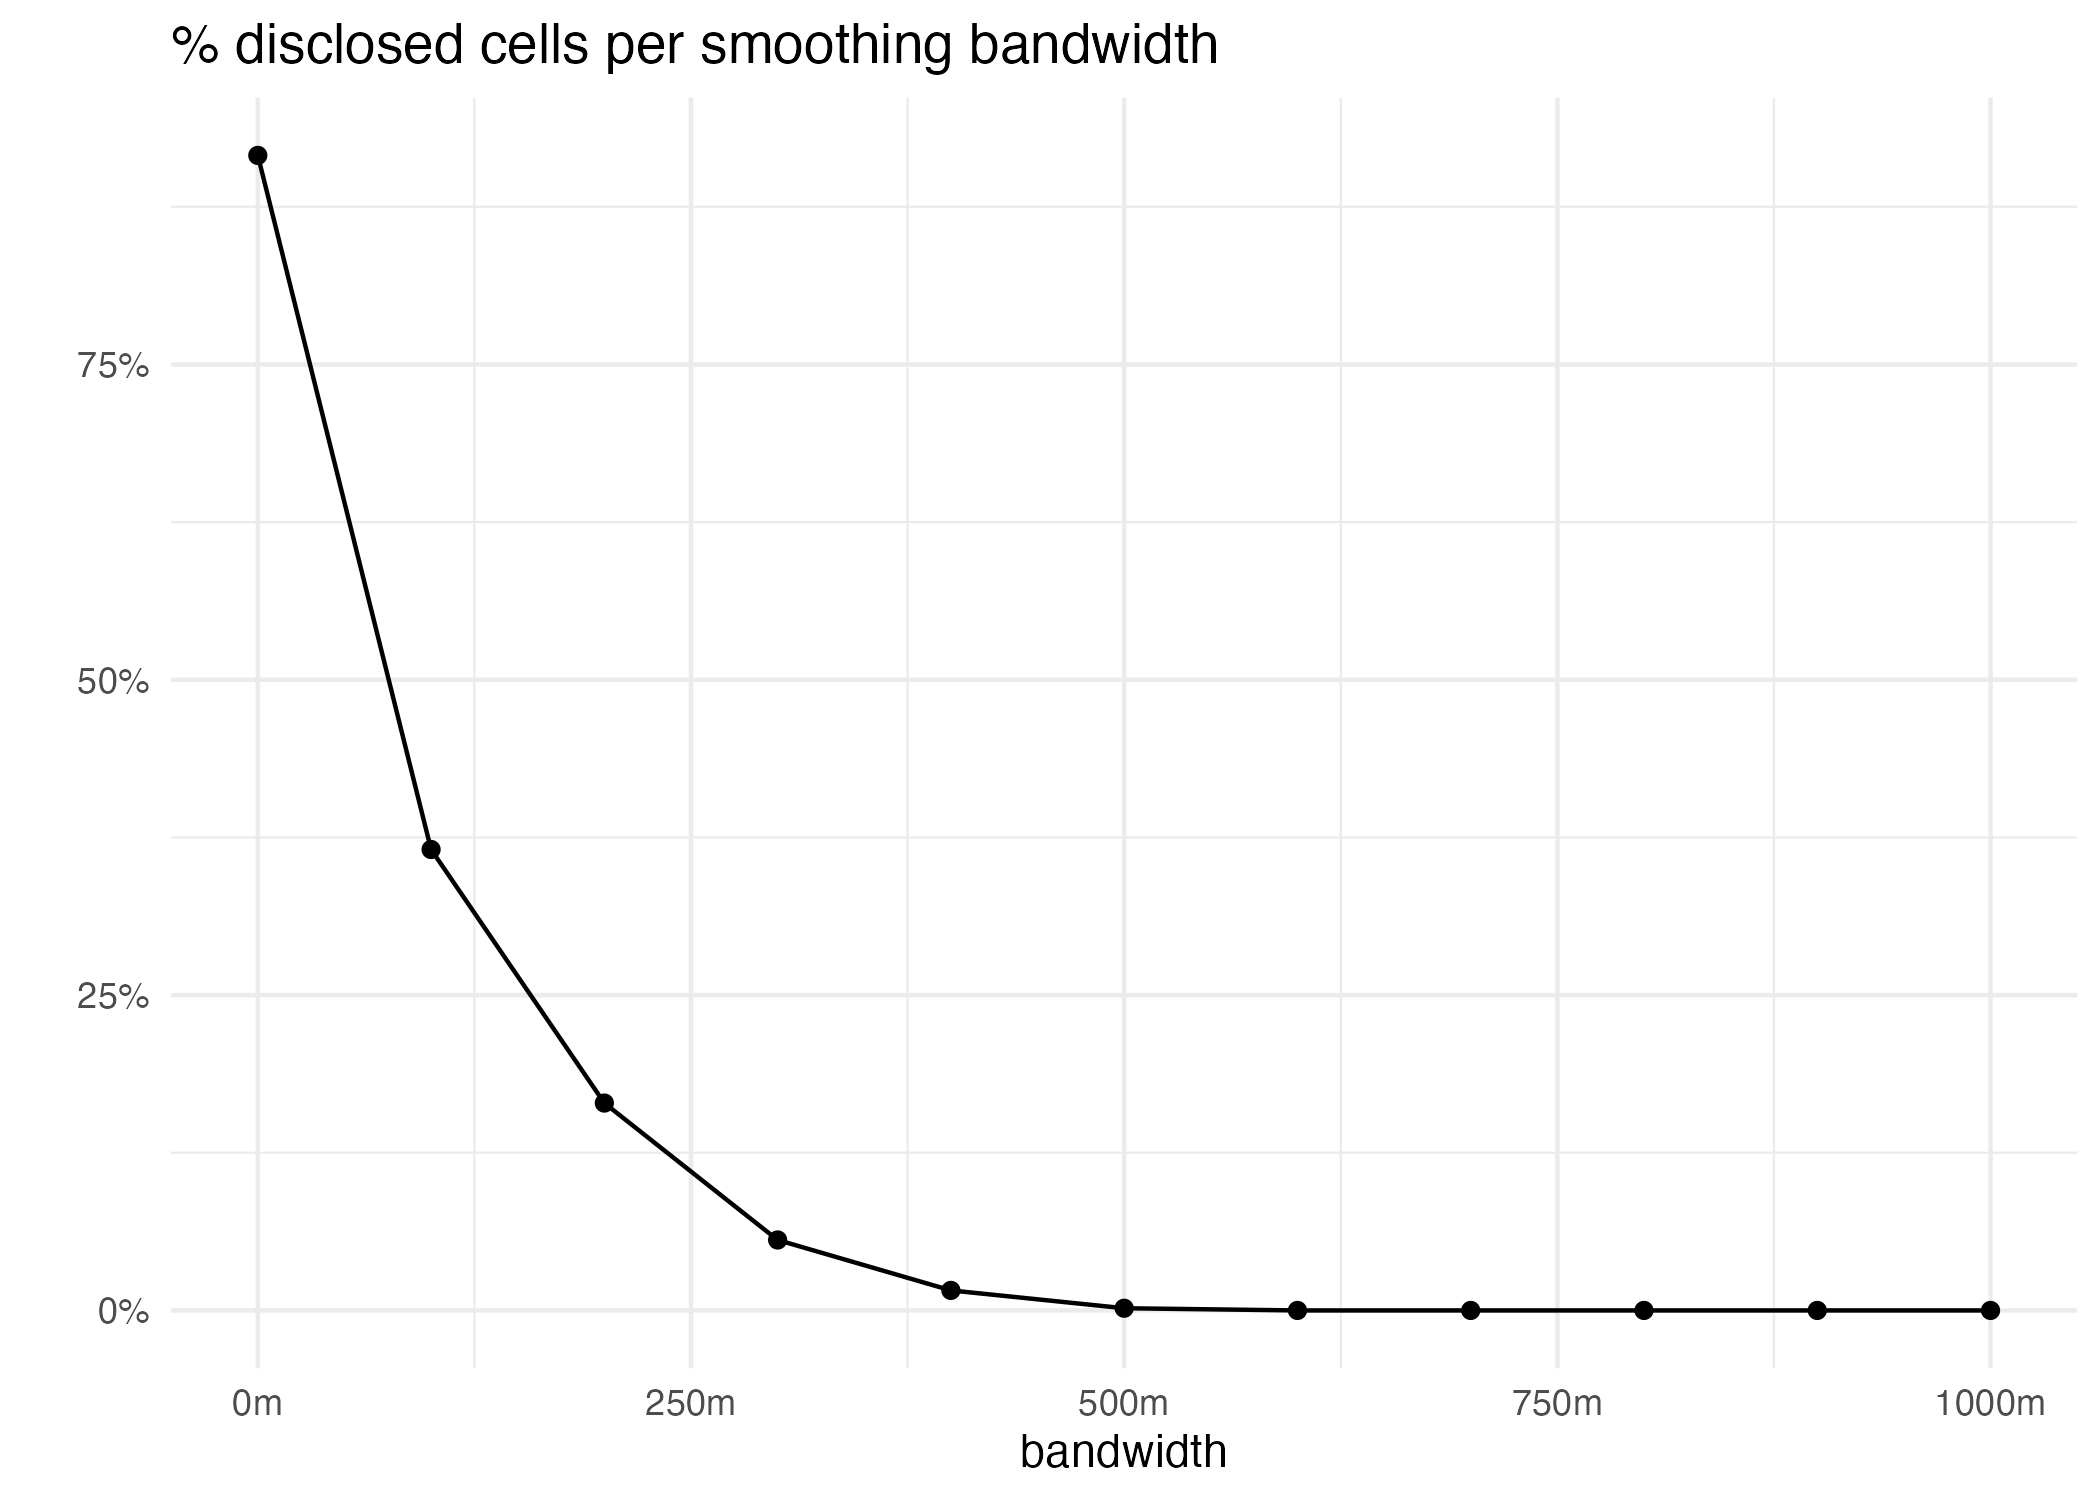
\includegraphics[width=.8\linewidth]{figures/Smoothing/sensitive_dep.png} 
    \caption{Unsafe locations as a function of the band width of the kernel density smoother.}
    \label{fig:sm_sensitive_bw}
\end{figure}

The trade off between risk and utility can be seen in figure~\ref{fig:sm_bandwidth}, which shows that for larger band widths, the spatial pattern is smoothed away. Interestingly enough smoothing with small band widths seems to improve visual utility, by improving spatial pattern. For the location utility measures however, it performs worse than 
other protection measures.

\begin{figure}[H]
    \centering
    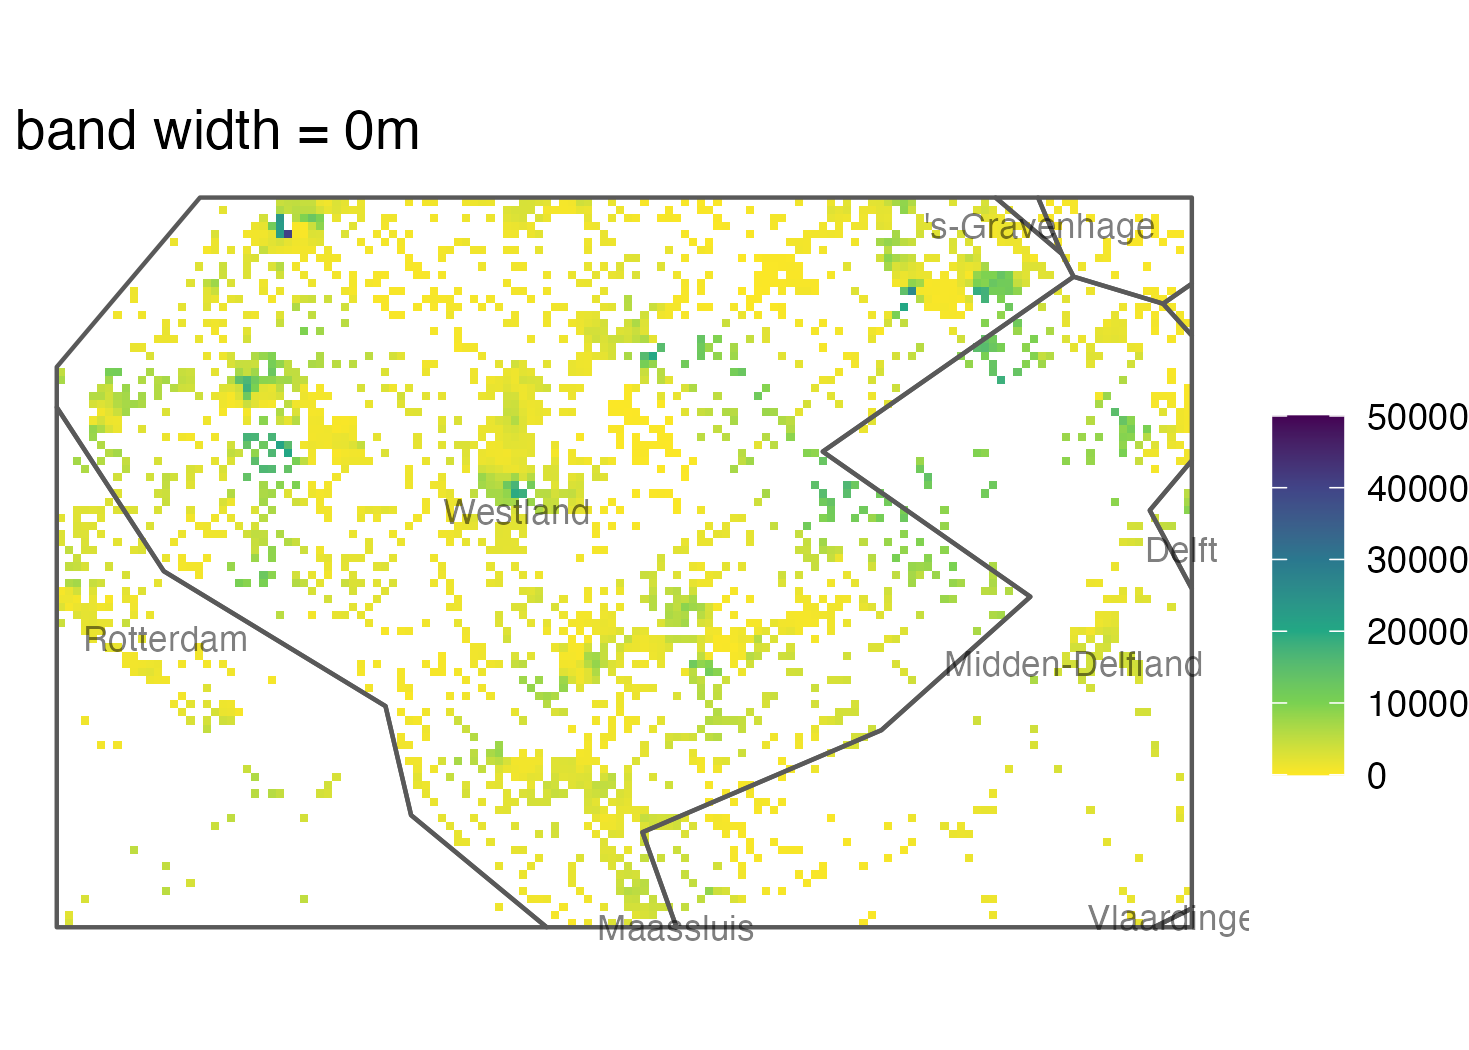
\includegraphics[width=.49\linewidth]{figures/Smoothing/fixed_smooth_0.png}
    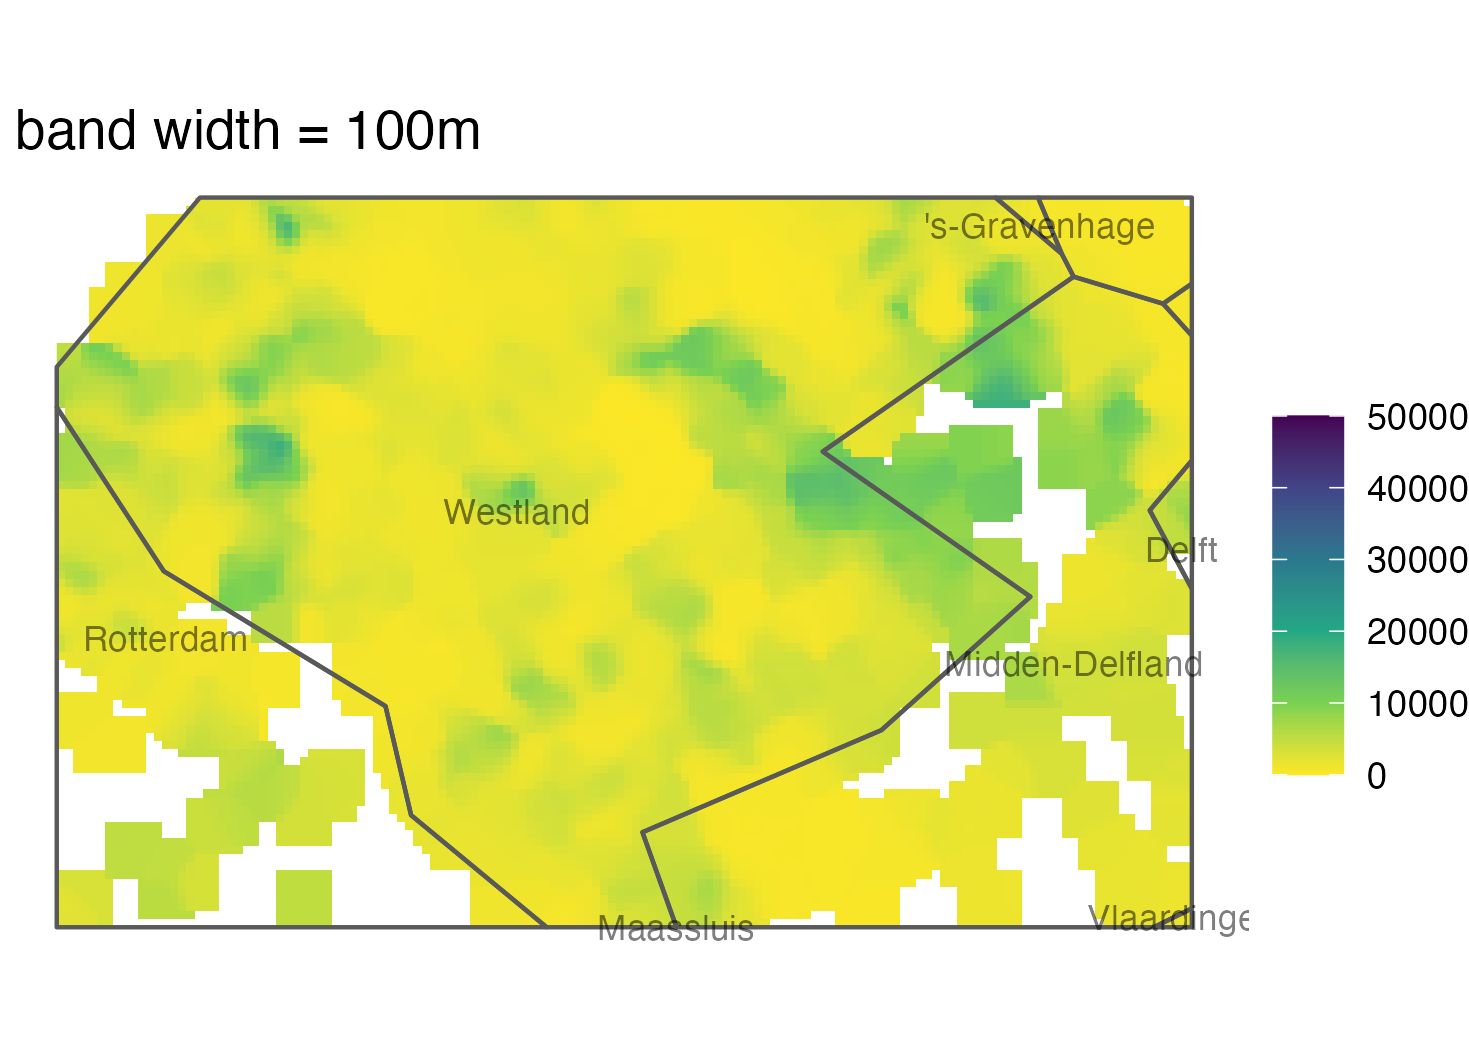
\includegraphics[width=.49\linewidth]{figures/Smoothing/fixed_smooth_100.png}\\
    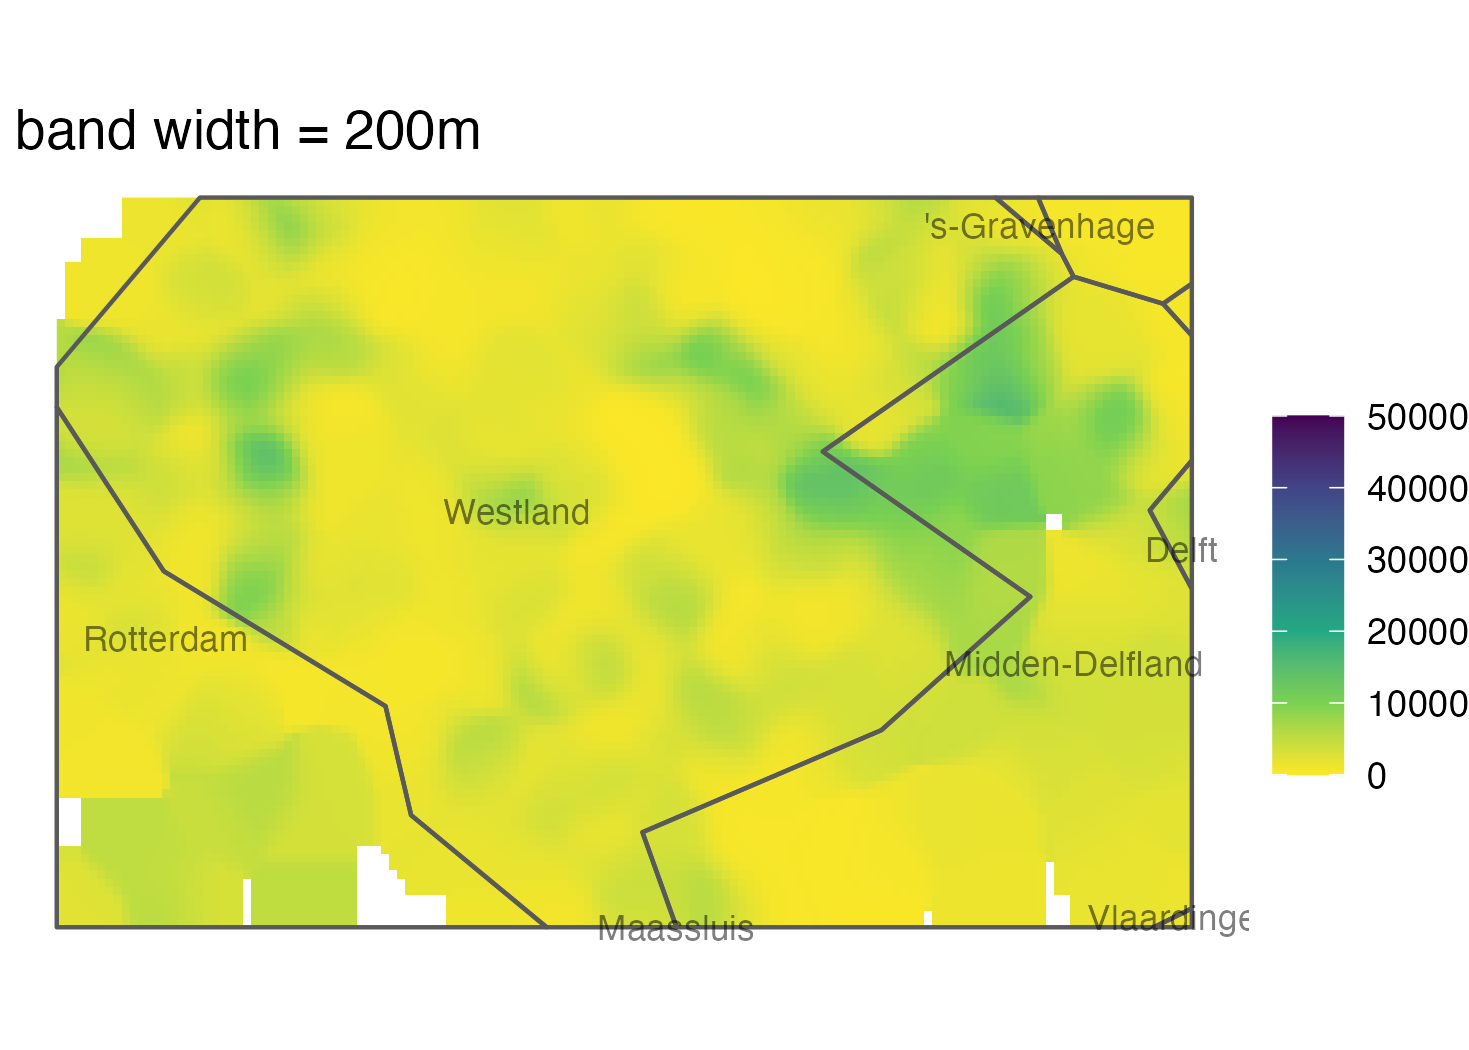
\includegraphics[width=.49\linewidth]{figures/Smoothing/fixed_smooth_200.png} 
    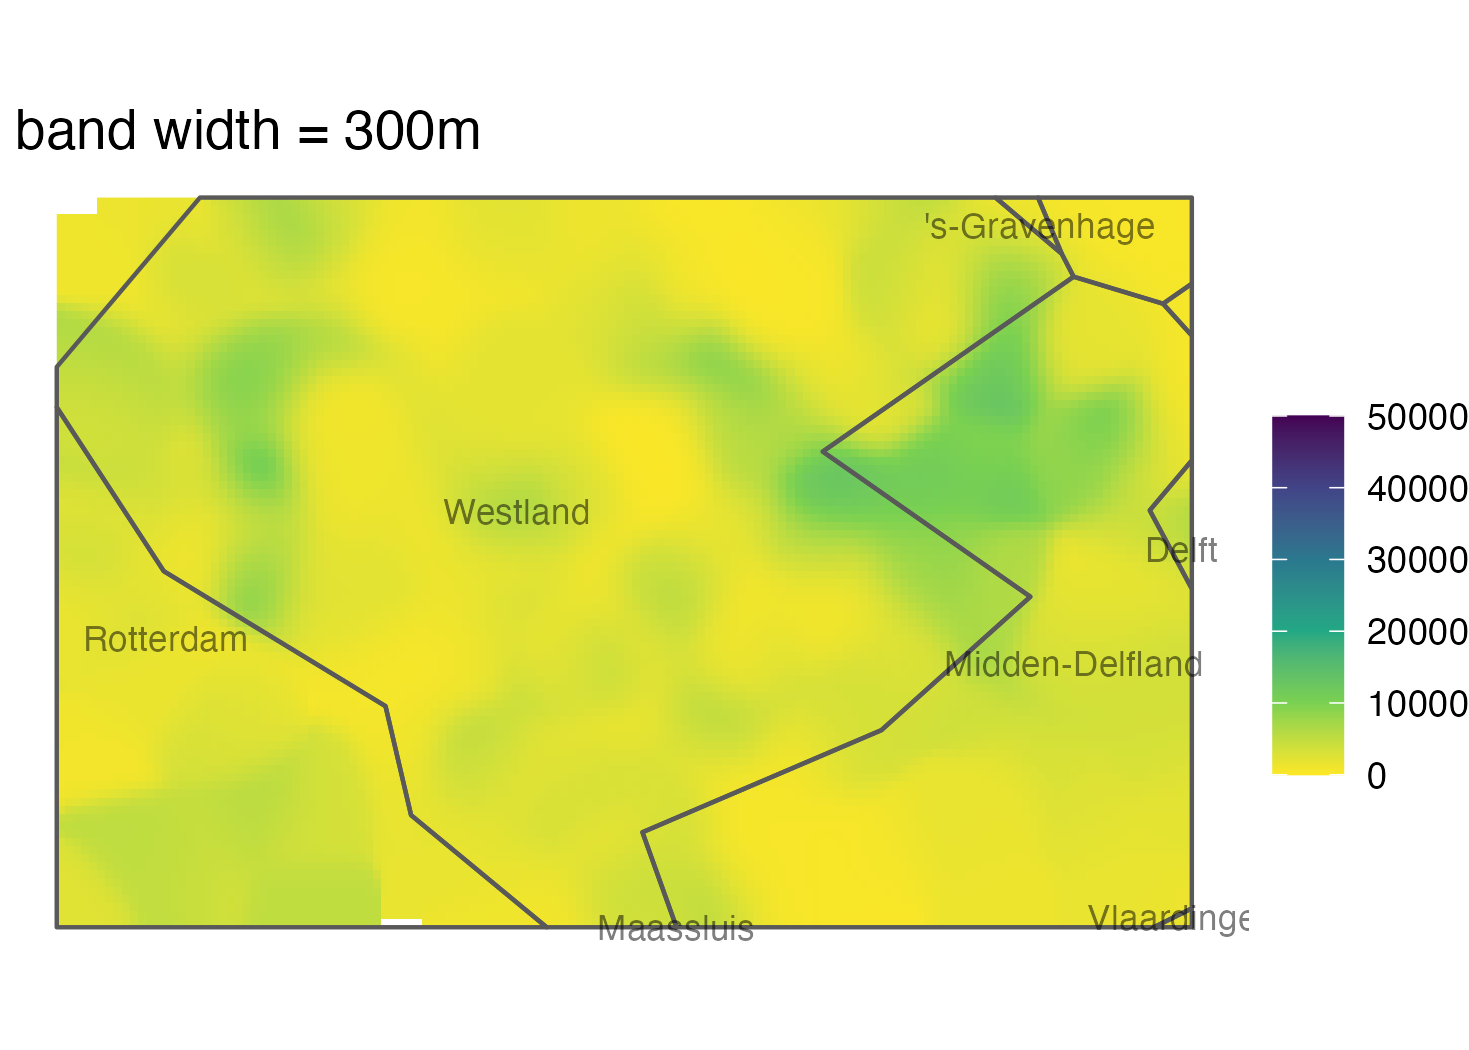
\includegraphics[width=.49\linewidth]{figures/Smoothing/fixed_smooth_300.png} \\
    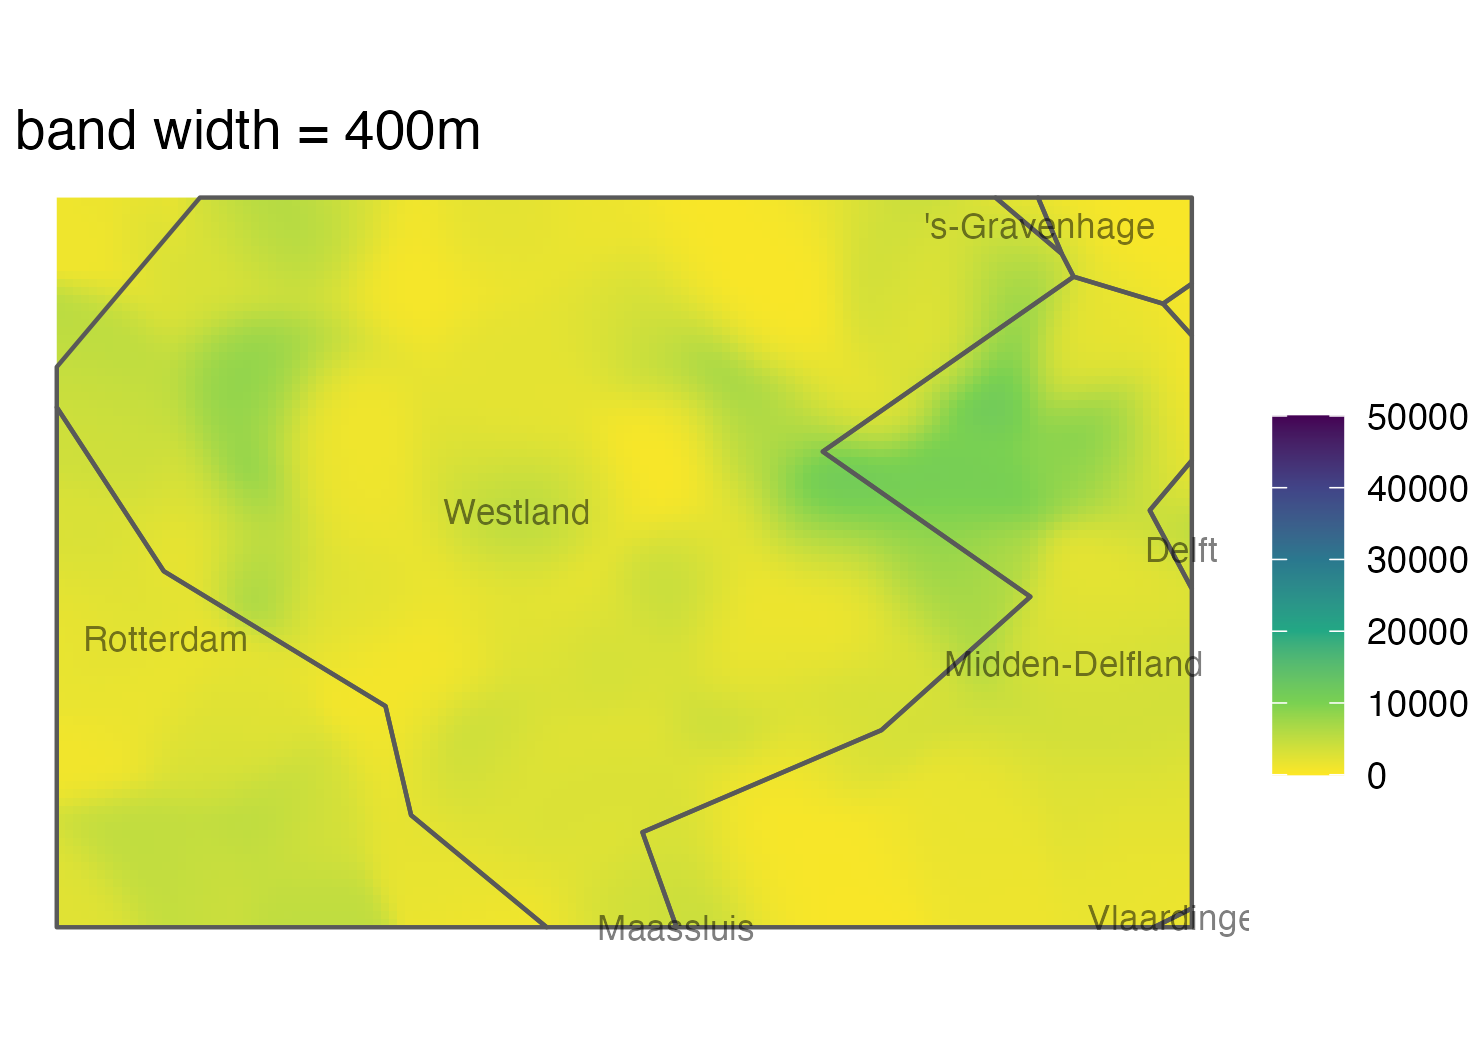
\includegraphics[width=.49\linewidth]{figures/Smoothing/fixed_smooth_400.png} 
    \includegraphics[width=.49\linewidth]{figures/Smoothing/fixed_smooth_500.png} 
    \caption{Spatial smoothing with increasing band width (0-500m).}
    \label{fig:sm_bandwidth}
\end{figure}

\subsection{Discussion}

An attractive feature of the kernel smoothing is that it both reveals the spatial patterns and better protects the individual observations. 
Two parameters are important for the disclosure control: band width and resolution of the data. Coarsening the grid is a simple solution for reducing disclosure risk, but also decreases utility as it quickly results in a blocky picture. 

The smoothing procedure in this section uses a fixed band width for the region. Since the spatial distribution of geographical phenomena in general is very skewed (e.g. the population densities of urban and rural regions are
very different), a variable or adaptive band width method might be interesting.

\subsubsection{Tools and Software}

Spatial smoothing for variable and population counts can be implemented with several R packages 
including \texttt{spatstat} \citep{spatstat_2005}, \texttt{btb} \citep{btb_2022} and \texttt{sdcSpatial} \citep{sdcSpatial_2022} which all assume georeferenced data. 

Spatial smoothing for population counts can also be accomplished using R packages \texttt{KernSmooth} \citep{kernsmooth_2024} and \texttt{MASS} \citep{mass_2002}.

The spatial smoothing method can be implemented using the R package \texttt{sdcSpatial} \citep{sdcSpatial_2022}. It includes options to specify the risk norms for the $p\%$ rule and the $(n,k)$ rules as well as the band width applied.
The package furthermore allows to assess the number of cells at risk and their removal.

\subsection{Summary}

Apply Spatial Smoothing to protect spatial density has the following advantages and disadvantages:

\noindent\emph{Advantages:}
\begin{itemize}
    \item Uses high density areas to protect nearby low density areas.
    \item Results in a smooth spatial density, which often aligns with publishing the data as a density map.
\end{itemize}

\noindent\emph{Disadvantages:}
\begin{itemize}
    \item Scores lower on utility measures compared to other methods.
\end{itemize}
    
\newpage
    \section{Cell Key Method} \label{sec:ckm}

The \emph{Cell Key Method (CKM)} is a post-tabular so-called `sticky' noise mechanism that perturbs aggregates. The treatment here is built on \citet[5.4]{HundepoolEtAl2024}, where a more detailed description can be found. The original idea goes back to \citet{FraserWooton2005}.
Notably, the spatial character of the data is not explicitly taken into account. Instead, the conceptual starting point is logical equivalence between a data product of small area aggregates (for example a grid map) and a table created by cross-tabulating with the small area identifier (e.g. the grid cell ID).
For instance, a cross-tabulation of persons as indicated in table \ref{tab:intro_exa} would yield three distinct, but interrelated grid maps (or, equivalently, a raster with three bands).
%: one with counts of persons below 50, one with persons aged 50 and above, one for the subtotal population count. 

\begin{table}[H]
    \centering
    \begin{tabular}{| c | c c | c |}
    \hline
        Grid Cell & Age $< 50$ & Age $\geq 50$ & Total\\
    \hline
         N:2698400 E:4339500 &  &  & \\
         N:2698400 E:4339600 &  &  & \\
         N:2698400 E:4339700 &  &  & \\
         \vdots & & & \\
    \end{tabular}
    \caption{Schematic example for two-way cross-tabulation with grid cells.
    %, equivalent to three grid bands (one per category of the column attribute, including right margin).
    }
    \label{tab:intro_exa}
\end{table}


\subsection{The CKM noise mechanism} \label{sec:ckm_mecha}

Maps of counts are common geospatial data products. We assume here that such products are created bottom-up by the aggregation of georeferenced statistical units (persons, households, or the like) to small areas, such as grid cells.

Formally, we number the population units $i = 1, \dots, N$ and the areas $j = 1, \dots, M$. The area to which a unit $i$ is assigned is $\mathcal{A}_i \in \{1, \dots, M\}$. For the Cell Key Method, each population unit furthermore has a random \emph{record key} in the form of a real number $\mathrm{rk}_i \in [0 \,, 1]$. When counts per area are compiled, we always perform two aggregation steps instead of one: Counting the number of units and summing their record keys equivalently. Formally:
\begin{equation}
\begin{aligned}
    X_j = \sum_{i=1}^N \mathbbm{1}(\mathcal{A}_i = j) \hspace{1.3cm} \forall j = 1, \dots, M \\
    \mathrm{ck}_j := \left(\sum_{i=1}^N \mathbbm{1}(\mathcal{A}_i = j) \cdot \mathrm{rk}_i \right) \mod 1 \hspace{1.3cm} \forall j = 1, \dots, M
\end{aligned}
\end{equation}
where $\mathbbm{1}(\,\cdot\,)$ is an indicator function, yielding 1 if unit $i$ is located in area $j$, 0 otherwise. Performing the operation `mod 1' keeps only the digits after the decimal point.\footnote{
    An equivalent expression is $\mathrm{ck}_j := \left (\sum_{i=1}^N \mathbbm{1}(\mathcal{A}_i = j) \cdot \mathrm{rk}_i \right ) - \left\lfloor \sum_{i=1}^N \mathbbm{1}(\mathcal{A}_i = j) \cdot \mathrm{rk}_i \right \rfloor$, where $\lfloor\,\cdot\,\rfloor$ is the floor function (rounding to next-lowest integer).
}
$\mathrm{ck}_j$ is the \emph{cell key} of area $j$. It determines the noise used for perturbation of the original value $X_j$. The perturbed value $X'_j$ is then the sum of original cell value and associated noise; formally: $X'_j = X_j + \Delta X_j(\mathrm{ck}_j)$. Specifically, the noise value $\Delta X_j(\mathrm{ck}_j)$ is read from a \emph{perturbation table} (or \emph{p-table} for short), depending on the original count and the cell key. For the design of the p-table and other details on the method we refer the reader to \citet[5.4]{HundepoolEtAl2024}.

The noise added by CKM to counts has the following important characteristics:
\begin{itemize}
    \item It has an expected value of zero (is unbiased). That means values do not get systematically smaller or larger. Furthermore, the method can be set up so that true zeros stay zero.
    \item It has a fixed variance and is bounded by a \emph{maximum perturbation value}. E.g. with a maximum perturbation of 5, the perturbed value is always within $\pm 5$ of the original value.
    \item It does not create negative counts (unless specified to do so). For example, to an original count of 2, no perturbation of $-3$ will be applied.
    \item Because it is built on cell keys, the noise is consistent across different aggregations. For example, if a grid cell and an administrative region happen to encompass exactly the same units, then aggregating by cell ID and by region ID will yield the same perturbed value (same units, same noise).
\end{itemize}


\subsection{Utility aspects} \label{sec:ckm_util}

\subsubsection{Non-additivity}

Since noise is applied independently to inner and marginal aggregates, those often do not add up exactly. This applies  for summing over both attribute data and the spatial dimension. For example, adding up the counts of native and non-native inhabitants in an area may produce a result that deviates slightly from the combined number of inhabitants.
Similarly, consider a population grid provided in two resolutions: 100m $\times$ 100m and 200m $\times$ 200m, where 4 small cells constitute a large one. Before CKM, summing the values of the 4 small cells yields that of the large cell. With CKM, a slight difference may result.

It is important to understand that non-additivity, though unusual at first, is actually a benefit in terms of data accuracy: Summing up perturbed inner cells to create totals would necessarily imply a larger error margin for these totals. Furthermore, consistency between tables would be hard to reach. Non-additive output allows CKM to guarantee consistency and the same sharp error bounds for values at all levels of aggregation.\footnote{
    Methods exist to restore additivity of perturbed tables ex post. They requires, however, significant computing effort and are only feasible for a small number of tabulations. Therefore, restoring additivity limits the flexibility of the approach and also tends to lead to higher information loss. For a more detailed discussion see \citet{EnderleGiessing2017}.
}
Nevertheless, the non-additivity property of CKM needs to be carefully explained to users. Recommendations and examples for this task can be found in \citet[~ch.5]{Guidelines3_CensusDemog}.

In rare edge cases, non-additivity can mean that a single category becomes larger than the subtotal. For instance, in an area we may have 20 native inhabitants and a single non-native inhabitant. By chance it can occur that the subtotal (native + non-native) is changed from 21 to 19, whereas the `native' count stays at 20. Such small inconsistencies are known from other methods like random rounding. Their likelihood depends on the skewness of the count distribution, the frequency of very small counts and on the maximum noise encoded in the p-table.

\subsubsection{Custom aggregates from noisy counts}

Since CKM perturbs values independently, adding up noisy values also adds up errors. Suppose, for instance, a city quarter is made up of 5 ZIP codes. Manually summing the 5 counts of inhabitants after CKM leads to a margin of error for the sum that is 5 times as high as that of a single count value. The issue is equivalent to that found in rounding methods; see also \citet[5.5]{HundepoolEtAl2024}. Summing up rounded values can lead to large errors; the suggested alternative is rounding the (true) sum. Similarly, with CKM it is strongly recommended that all aggregates of interest (e.g. the count for the city quarter as a whole) are computed beforehand and CKM applied to them directly. The error for the marginal value is then bounded by the same maximum perturbation value as the contributing inner values.
What is described here for custom sums also holds, of course, for custom differences. This is in fact an eminent aspect of the method, needed to protect against differencing (see section \ref{sec:ckm_risk}). 
%Nevertheless, this issue may limit certain data products.\footnote{
    %For example, an interactive grid map that allows users to freely select any number of cells and display the sum of noisy cell counts would be afflicted in the way described here.}

\subsubsection{Ratios of noisy counts}

The spatial distribution of pretty much all counts is strongly correlated to that of the overall population count. This is a common issue in the creation of statistical maps. For example, mapping the number of people above a certain age threshold tends to approximately replicate the general population distribution, which is not very informative. Better information is conveyed by mapping \emph{ratios} -- like the share of old people among all inhabitants.

For these ratios we may use noisy counts in both the enumerator and denominator, i.e. $X'/Y'$ instead of $X/Y$. If the counts involved are small, the relative error in both can be relatively large and hence the ratio may be unreliable. The problem is discussed in detail in \citet{EnderleEtAl2018}. Generally speaking, if the counts involved are large, then the ratio will be accurate. If either or both counts are small, accuracy may be low. When plotting a map of ratios, the count distribution of enumerator and denominator should be assessed for the same region in order to identify if and where such problems may occur. Areas with small counts can then, for instance, be marked by a flag as `imprecise', or the spatial support can be scaled up (e.g. from 100m $\times$ 100m to 500m $\times$ 500m grid cell) to ensure a smaller relative error throughout.

\subsubsection{False-empty cells}

Safe aggregates usually require protection of \emph{small counts}. In order to assure that added noise is unbiased it is often required that such small values have a certain probability of being perturbed to \emph{zero}. Changing very small counts (for instance 1 or 2) to 0 can even be an explicit requirement for the p-table to ensure sufficient protection \citep{GiessingHoehne2010}.
However, if one then treats areas with artificial zero-counts the same way as originally unpopulated areas, this slightly distorts the spatial pattern in sparsely populated areas. The issue somewhat mirrors that of \emph{suppressing} small counts.

\subsubsection{CKM and the Modifiable Areal Unit Problem}

As noted above, the perturbation that CKM adds to a true count is defined in absolute terms, hence the expected \emph{relative} perturbation depends on the level of aggregation. A map of many small counts is changed relatively more than a map of a few large counts. This is independent of the number of \emph{sensitive} cells (as per the criteria in \ref{sec:risk_aggr}), since CKM does not distinguish between sensitive or non-sensitive values.

\subsubsection{Treating hierarchical relations between units}

It is not uncommon that data is collected on several hierarchically linked, jointly geo-referenced units. The most common example is a population and housing census, where we assume n:1 relationships (one or more people per building, exactly one building per person).\footnote{
    Geo-references in census contexts are assigned by address, hence the lower-level unit (person, family, or household) inherits its geo-reference from the higher-level unit (building).} 
There is therefore a logical connection: if an area contains at least one person, it \emph{must} contain at least one building. We often want to preserve such logical connections as much as possible. For instance, it would be inconvenient if the person count in a small area were changed from 1 to 0, but the corresponding building count from 1 to 3. This would violate the constraint that all buildings must contain at least 1 person. But it can happen if record keys are drawn independently for both types of units.
A small example is shown below: records for two types of units (persons and buildings) are held in separate microdata files, but linked by IDs. Record keys are first drawn independently for both data sets.

Consider the units located in grid cell (N:100 E:100) in the example data (shown in blue). If we aggregate separately persons and buildings by grid cell as explained in \ref{sec:ckm_mecha}, we get counts of 1 in each case with cell keys of 0.1265\dots and 0.8910\dots respectively. Depending on the p-table this could lead to a situation as described before, where the number of buildings is increased, that of persons changed to zero.
Such paradoxes cannot always be prevented. However, we can limit their occurrence. 

\begin{table}[H]
    \centering
    \begin{tabular}{| c | c | c | c |}
    \hline
        Person ID & Building ID & Grid Cell & Record Key \\
    \hline
            \textcolor{blue}{1} & \textcolor{blue}{1} & \textcolor{blue}{N:100 E:100} & \textcolor{blue}{.126547051} \\
    \hline
            2     &   2      &     N:200 E:100     & .650998366 \\
    \hline
            3     &   2      &     N:200 E:100     & .078194553 \\
    \hline
            4     &   2      &     N:200 E:100     & .970612172 \\
    \hline
            5     &   3      &     N:200 E:100     & .507300613 \\
    \hline
            6     &   3      &     N:200 E:100     & .040133080 \\
    \hline
    \end{tabular}\\ \vspace{10pt}
    \begin{tabular}{| c | c | c |}
    \hline
        Building ID & Grid Cell & Record Key \\
    \hline
          \textcolor{blue}{1} & \textcolor{blue}{N:100 E:100} & \textcolor{blue}{.891086490} \\
    \hline
          2      &    N:200 E:100      & .689734612 \\
    \hline
          3      &    N:200 E:100      & .479127417 \\
    \hline
    \end{tabular}
    %\caption{Caption}
    %\label{tab:my_label}
\end{table}

This time, we only draw record keys for persons. The record key for buildings is created in a pre-aggregation step as the cell key derived from aggregating persons by building.\footnote{
    E.g. the (new) record key of building 3 would be $.5073\ldots + .0401\ldots = .5474\ldots$, the sum of the record keys of its two inhabitants from the `person' microdata.
}

\begin{table}[H]
    \centering
    \begin{tabular}{| c | c | c | c |}
    \hline
        Person ID & Building ID & Grid Cell & Cell Key \\
    \hline
            \textcolor{blue}{1} & \textcolor{blue}{1} & \textcolor{blue}{N:100 E:100} & \textcolor{blue}{.126547051} \\
    \hline
      \{2, 3, 4\} &   2      &     N:200 E:100     & .699805091\\
    \hline
      \{5, 6\}    &   3      &     N:200 E:100     & .547433693 \\
    \hline
    \end{tabular}\\ \vspace{10pt}
    $\Rightarrow$ \quad
    \begin{tabular}{| c | c | c |}
    \hline
        Building ID & Grid Cell & Record Key \\
    \hline
          \textcolor{blue}{1} & \textcolor{blue}{N:100 E:100}  & \textcolor{blue}{.126547051} \\
    \hline
          2      &    N:200 E:100      & .699805091 \\
    \hline
          3      &    N:200 E:100      & .547433693 \\
    \hline
    \end{tabular}
    %\caption{Caption}
    %\label{tab:my_label}
\end{table}

This way of treating n:1 relations in the data can have several advantages. 
\begin{itemize}
    \item The danger of showing a cell as inhabited for one unit, but uninhabited for the related one, is lowered.
    \item The approach naturally generalizes to nested hierarchies (persons in a household, households in a house, etc.)
    \item It is often inherently desirable to treat logically equivalent aggregates the same in perturbation. For instance, a count of single-person households would be perturbed the same as the count of single persons within these households. By building record keys in intermediate aggregation steps, such 1:1 relationships are guaranteed to receive the same noise.
\end{itemize}  

\subsection{Risk aspects} \label{sec:ckm_risk}

CKM creates uncertainty about the true value of all area aggregates. While the uncertainty must be small enough to allow for reliable information, it must also be large enough to protect sensitive cells. This trade-off is realized by a given parameterization of the p-table -- for a detailed discussion see \cite[~ch.4]{Guidelines3_CensusDemog}. To discourage attempts of inferring true values, the central parameters (here: noise variance and noise maximum) are generally not published. 
%\citep{DupreEtAl2022}.

\subsubsection{Protection of small counts}

Areas with associated count values of 1 or 2 are often considered particularly sensitive, as noted in section \ref{sec:risk_aggr}. The CKM parameters can be set up in such a way that no 1s or 2s remain in the output. For example, with a maximum perturbation value of 3 a true area count of 2 may appear as 0, 3, 4, or 5, each with a certain probability. If we still allow 1s or 2s in the output, the method makes it uncertain whether they are veridical: Assuming again a maximum perturbation of 3, an observed 1 could have been a 1, 2, 3, or 4 before perturbation.

\subsubsection{Protection against geographic differencing}

To protect against the issue of geographic differencing (see section \ref{sec:risk_diff}), CKM relies on the loss of accuracy for custom sums and differences described in the previous subsection. In fact, this form of protection was the original intent behind the method, as proposed by \cite{FraserWooton2005}.

Consider the case of a single area $\mathcal{A}$, fully encompassed by another $\mathcal{B}$; the area values are $X_{\mathcal{A}}$ and $X_{\mathcal{B}}$. The value of the residual area $X_{\mathcal{B}\setminus\mathcal{A}} = X_{\mathcal{B}} - X_{\mathcal{A}}$ is the target of differencing. When CKM is applied, both area values are perturbed \emph{independently} to $X'_{\mathcal{A}}$ and $X'_{\mathcal{B}}$, as described in section \ref{sec:ckm_mecha}. The noise %$\Delta X$ 
added to an original $X$ to derive  the perturbed $X'$ has a given fixed variance encoded in the p-table.
%; we denote it by $\mathrm{Var}(\Delta X)$
By standard results, the noise of the difference $X'_{\mathcal{B}\setminus{\mathcal{A}}} = X'_{\mathcal{B}} - X'_{\mathcal{A}}$ has twice the variance of the noise of the individual components.
%has variance $\mathrm{Var}(\Delta X) + \mathrm{Var}(\Delta X)$, twice as high as for any of the single area aggregates.
The same holds for the maximum perturbation value.\footnote{
    Suppose the perturbed values $X'_{\mathcal{A}}$ and $X'_{\mathcal{B}}$ are within $\pm 5$ of their respective original values. Then the difference $X'_{\mathcal{B}} - X'_{\mathcal{A}}$ can vary between $-10$ (both $X_{\mathcal{A}}$ and $X_{\mathcal{B}}$ perturbed with $-5$) and $+10$ (both $X_{\mathcal{A}}$ and $X_{\mathcal{B}}$ perturbed with $+5$) around the true differenced value.}
If the two area systems were perturbed with different p-tables, each having its own variance and maximum perturbation value, the variance and maximum of the noise for the difference would be given by the sum of the variances and maxima respectively. Even if one of the area values (encompassed or encompassing) is perturbed and the other is not, the differenced value inherits the uncertainty associated with the perturbed area. 
The uncertainty around the differenced value is even higher, if either the encompassing or the encompassed area is a combination of several smaller areas.\footnote{
    For instance, suppose we sum the values of 10 different grid cells to derive an encompassing area around an administrative region and both the grid data and the administrative data is protected by CKM noise with constant variance $\mathrm{Var}(\Delta X)$ and maximum perturbation value $D$. Then the differenced value has variance $(10 + 1) \cdot \mathrm{Var}(\Delta X)$ and is within $\pm (10 + 1) \cdot D$ of its true value. The more independently perturbed values are contributing (i.e. the more complex the differencing), the higher the uncertainty of the result.}
CKM thus generally provides effective protection against geographic differencing.\\

As with all disclosure control methods, there exist edge cases where the protection is less than ideal. In general, knowledge of the maximum perturbation value allows the computation of feasibility intervals. It is suggested that the CKM parameters are not made public. Furthermore, certain rare cases can still allow successful differencing, especially when inner and outer area are both perturbed by the maximum amount, but in opposite directions. Such issues can (and should) be taken into account when setting up the p-table, as described in \cite{EnderleEtAl2020}.\\

When aggregates are published for several, partially overlapping geographies, it is important to compute them from the same microdata. Logically identical aggregates then receive the same cell key and therefore the same noise. For instance, if all people in a village belong to the same postal code, aggregating their record keys once by the village's official regional key, once by postal code, yields in both cases the same cell key, as intended. If both sets  of geographic information are kept in \emph{separate} microdata files, one should \emph{not} draw two independent sets of record keys, but rather (a) draw them for one, then join them to the other, or (b) combine the data sets, then draw record keys. Otherwise we could end up with two (or more) values for one and the same ground truth. 
This would be both confusing as well as a potential risk factor, since it provides more information on the true confidential value.

\subsection{Tools and Software}

The Cell Key Method can be implemented using the $\tau$-\emph{Argus} software \citep{QuickRefTau42x} or the R package \texttt{cellKey} \citep{cellkey_meindl}. The former tool includes some information loss measures and some visual feedback on the added noise using graded colors. The latter tool also includes convenience functions, like automatically computing several information loss statistics.
In either case, the p-table must be supplied. For its creation the R package \texttt{ptable} may be used. For both R packages, useful vignettes are found online to get users started.\bigskip

%\subsection{Summary} \label{sec:ckm_summa}

%In summary, applying CKM to protect small area aggregates has the following advantages and disadvantages:\\

%\emph{Advantages:}
%\begin{itemize}
%    \item Effective protection against differencing, including geographic differencing.
%    \item Published totals and subtotals have the same accuracy as inner values; since they are perturbed independently, errors do not build up.
%    \item Allows for comparatively flexible tabulation / mapping of spatial data. Change of Support problems (like with local aggregation of areas) are avoided.
%    \item If the perturbation table is set up such that counts of zero are not perturbed, there will be no artificially inhabited cells. Avoids implausible locations, since values are not moved in space, just increased or decreased. Works for isolated areas (does not need populated neighbourhood).
%    \item Coherent across multiple data products / publications (same units, same noise).
%\end{itemize}
%\emph{Disadvantages:}
%\begin{itemize}
%    \item Not additive. Inner cells can (by chance) become larger than marginals.
%    \item Manually calculated aggregates over several perturbed areas (e.g. sums of perturbed grid cells) can come with large errors. Same holds for derived statistics of two or more independently perturbed values for the same area (like ratios).
%    \item Might create artificially uninhabited cells.
%    \item Changes also values of cells that are not at risk.
%    \item Risks of successful averaging attacks \citep{AsgharKaafar2020} should be controlled. This is done by considering the complexity and flexibility of the planned outputs when choosing method parameters \citep{Bach2022}.
%\end{itemize}

Case studies from different countries that apply the Cell Key Method to geographic grid data are \citet{Kraus2021}, \citet{Dekany2019}, as well as \citet{LukanSmukavec2017}. A reproducible application to a chunk of German census-like grid is provided in this document in section \ref{sec:cs_ckm}.

A summary of strengths and weaknesses of the Cell Key Method can be found in section \ref{sec:strengthweak}.

\newpage

    \section{Targeted Record Swapping} \label{sec:trs}

Targeted Record Swapping (TRS) is a pre-tabular perturbation method. Its intended use is to apply a swapping procedure to a micro data set before generating a table.
For a general outline of the method see \citet[5.6]{HundepoolEtAl2024}.

Although TRS is applied solely on micro data, it is first of all considered a protection method used for tabular data. However, it can also be applied, of course, for protecting the micro data itself, although the experience to date indicates that it should not be used alone in this case: the swapping of pre-defined groups of units (spatial area, households, groups of economic entities, etc.) may not provide fully effective protection, and some additional perturbative tools -- e.g. microaggregation \citep[3.4.5]{HundepoolEtAl2024} -- may be needed. For an example of a combined application of protection methods, including TRS, to protect micro data see \citep{Mlodak2022}.
TRS can be used for tables with and without spatial characteristics, with the prior case containing also grid data products or tables created by cross-tabulating with grid cells.   
When applying TRS, the spatial character of the data can be taken into account to some degree. 


\subsection{The TRS noise mechanism}

TRS is applied directly to the underlying micro data before generating any table. As a consequence, the methodology of TRS is not dependent on the final table, be it count data or a magnitude table.

Given are a number of units $i = 1, \ldots, N$ in a population, where each unit $i$ has $q$ characteristics or variables $\{x\}_{i,j} = \mathbf{X} \in \mathbb{R}^{N\times q}$.
In addition, there exists a geographic hierarchy $\mathcal{G}^{1} \succ \mathcal{G}^{2} \succ \ldots \succ \mathcal{G}^{K}$ and each unit $i$ can be assigned to the $m$-th unique area $g_m^{k} \in \mathcal{G}^{k}$ in each hierarchy level $k$, $k=1,2,\ldots,K$.\footnote{
    Depending on type and aim of the survey, the geographic hierarchy can be replaced here by another pre-defined hierarchy of groups of units, e.g. levels of a given key classification.}

Risk values $r_{i,k}$ can be computed for each unit $i$ for each geographic level $k$, given the geographic hierarchy and a set of variables $\{x\}_{i,j}$.
For an overview on such record-level risk measures see, for instance, \citet{GregoryOfer2011} or \citet{Skinner2009}.
Additional, use-case specific parameters needed for the noise mechanism of TRS are:
\begin{itemize}
  \item A global swap rate $p$;
  \item A risk value $r_{high}$ beyond which all units with $r_{i,k}$ are considered \textbf{high risk} for the geographic hierarchy level $k$;
  \item A set of variables $\mathbf{x}_1,\ldots,\mathbf{x}_s$, available for each unit $i$, which are considered for similarity while swapping units. 
\end{itemize}

Starting at the highest hierarchy level $\mathcal{G}^{1}$, units $j$ for which $r_{j,1} \geq r_{high}$ are selected and randomly swapped with units belonging to other geographic areas at the first hierarchy levels.
The selection is chosen by randomly selecting units using $r_{i,k}$ as sampling weights. In addition, variables $\mathbf{x}_1,\ldots,\mathbf{x}_s$ are respected during the selection such that the units which are swapped have the same value for these variables.
Iterate through all succeeding hierarchy levels in the same fashion. At the last hierarchy level, additional units with $r_{i,K} < r_{high}$ are swapped to reach $p\cdot N$ overall swapped units.



\subsection{Utility and risk aspects}

TRS is applied on the micro data before constructing any tables or maps. The swapping of micro data records specifically targets records with higher risk of disclosure with respect to the dimensions of the final output.
In the case where multiple maps are produced from the same micro data, it is recommended to apply the TRS only once and use the same perturbed micro data for all maps. This results in a delicate balance between utility and number of records swapped for each of the maps, as it is difficult to address many disclosure risks from different maps or tables while applying TRS only one time. 

TRS is usually applied in such a way that the records swapped with each other are the same in numbers. That is, individuals or households of the same size are swapped with each other. Using TRS to protect a map or a grid data product displaying the total population is therefore ill-advised. TRS should only be considered if final maps contain a subset of the perturbed micro data set or the maps display an additional demographic dimension.  

As for any method, it is advised to thoroughly tune parameters to balance information loss and disclosure risk. Possible tuning parameters are:

\begin{itemize}
\item The hierarchical depth $K$;
\item The construction of the risk values $r_{i,k}$ and $r_{high}$; 
\item The choice of $\mathbf{x}_1,\ldots,\mathbf{x}_s$; 
\item The global swap rate $p$.
\end{itemize}

\noindent Both the hierarchical depth $K$ as well as $r_{i,k}$ and $r_{high}$ directly influence the overall number of swaps done during the procedure. A detailed hierarchy can imply many units with high risk on a low hierarchical level, which in turn leads to a larger number of swaps. Analysing the distribution of risk values on the lowest hierarchical level $r_{i,K}$ can give a good overview on the expected minimum number of swaps, overall and per geographic region. Overall, at least 
%$\lceil \frac{\#\{i:r_{i,K}\geq r_{high}\}}{2N} \rceil$
$\left\lceil (\#\{i:r_{i,K}\geq r_{high}\}) \,/\, 2N \right\rceil$
swaps can be expected. This estimate also indicates whether the hierarchical depth $K$ might already be too detailed for the protection purpose.\newline

\noindent The global swap rate $p$ can be choosen by estimating a pre-defined set of statistics per geographic region with varying $p$. A possible \textit{optimal} $p$ could be the maximum $p$ where this set of statistics remains \textit{similar} enough to the original estimates.
As a rule of thumb, with a swap rate beyond 10\% the final information loss will in general be very high.\newline

\noindent The set of variables $\mathbf{x}_1,\ldots,\mathbf{x}_s$ controls how similar swapped records are and thus can control the information loss to some extent. A very detailed set, however, can lead to no donor being found and thus failing to supply protection for the final tables. For real life applications it is usually favourable to supply multiple sets $\{\mathbf{x}_{t(1)},\ldots,\mathbf{x}_{t(s)}, t=1,\ldots , T\}$, such that units can be swapped if they agree on a very detailed set of variables, but if no donor is found, a less detailed set will be chosen to compare on. For real life applications, $T$ as well as $s$ will likely not be larger than 5. This functionality is implemented in the tools for TRS presented in \ref{sec:trstools} below. \newline

\noindent Because the noise is applied to the micro data before building any tables, additivity between inner and marginal aggregates will always be preserved.
Due to the design of the noise mechanism, TRS can not populate previously unpopulated cells. However, this does not hold for sub-populations, e.g. the number of individuals times citizenship by 1km grid cells.  

\subsection{Tools}\label{sec:trstools}

The TRS noise mechanism is implemented in the R package \texttt{sdcMicro}, function \texttt{recordSwap()}, as well as in $\mu$-Argus, alongside a multitude of parameters to fine-tune the procedure. Both R and $\mu$-Argus use the same implementation written in C++, which is available on GitHub\footnote{
    https://github.com/sdcTools/sdcMicro/tree/master/src/recordSwap}.
By default, the implementation applies $k$-anonymity to calculate risk values for each unit at each geographic level. This can, however, be changed by supplying pre-calculated risk values to the procedure.
The computation of information loss is supported in the R-package \texttt{sdcMicro} with the functions \texttt{IL\_variables()} and \texttt{infoLoss()}.

%\subsection{Summary}

%Applying TRS to protect geo-referenced data has the following advantages and disadvantages:

%\noindent\emph{Advantages:}
%\begin{itemize}
%    \item Method is simple to communicate.
%    \item Consistency between maps built from the same micro data set
%\end{itemize}

%\noindent\emph{Disdvantages:}
%\begin{itemize}
%    \item Fine-tuning TRS to protect multiple maps built from the same micro data set can be challenging.
%    \item Final maps might need an additional protection method.
%\end{itemize}
    

\newpage

    \section{Auxiliary Methods} \label{sec:aux}

\subsection{Binning values} \label{sec:aux_bin}

It can be helpful for protection to sort counts or continuous values into \emph{discrete class bins}. For example, in a map that shows local unemployment rate at the grid cell level, one may show for a cell not the value 12.5\%, but instead the class label `10-15\%'. The effect is similar to rounding, in that the user can only infer an interval for the true value; see \citet[5.5]{HundepoolEtAl2024}. Secondary disclosure risks are thereby also similar to deterministic rounding. 

\begin{tcolorbox}[breakable]
\emph{Example}:
Suppose we know from another map that the grid cell with class label `10-15\% unemployed' has a total of 8 persons in it. This reveals that 1 person is unemployed, since 1 in 8 is the only count that leads to a fraction between 10-15\%.
\end{tcolorbox}

For such reasons binning alone will often not suffice to create a safe geo-referenced data product. Instead, it is often advisable to use binning as an auxiliary method for post-processing the output from another SDC method. For example, \citet{JongeWolf2016} suggest discretising the density map from spatial smoothing (see section \ref{sec:methods_smooth}). Some general recommendations to increase the protection from binning are:
\begin{itemize}
    \item Choosing large enough uncertainty intervals.
    \item Curating the release program. For instance, the disclosure from unemployment rates in the example above relied on an additional release of true counts for the same grid.
    \item Avoiding intersecting or custom bins. For instance, releasing the same grid cell in two maps, where it is labeled in one `10-15\% unemployed' and `12\% or more unemployed' in the other, allows inferring that the true value must be in the interval 12-15\%, which is sharper than any of the two.
\end{itemize}

\subsection{Suppressing cell values} \label{sec:aux_suppr}

When aggregates for small geographical regions, such as grid cells, are considered unsafe for publication, the corresponding value may be suppressed -- meaning the value is kept from the publication and replaced by a suppression symbol, like a dot or `$\times$'. Thus replacing unsafe values is called \emph{primary suppression}. 
%Suppressed values are typically marked with a specific symbol in tabular representation, and with a specific color in choropleth maps to distinguish them from empty cells.

If aggregates are published in nested area systems (for instance 100m $\times$ 100m grid cells and 200m $\times$ 200m grid cells), then the suppressed value may still be disclosed by subtraction. For instance, if from the four nested cells that make up a large cell, a single one is suppressed, one would only need to subtract the value of the other three from the value of the large cell. To prevent this, at least \emph{two} suppressed cells are required within the larger cell. The value of the large cell is equivalent to a `column total' (or sub total) in a table. At the same time there may be a `row total' along the subject domain: We may publish, for instance, counts of total population, native population and non-native population per grid cell. If we suppress the value of `non-native' for an area, we must suppress that of `native' as well in order to prevent disclosure by subtraction. The problem of \emph{secondary suppression} from statistical disclosure control for tables therefore applies. The reader is referred to \citet[ch. 4]{HundepoolEtAl2024} for details.

Some further remarks on cell suppression in the geographic context:
\begin{itemize}
    \item Grid products for whole countries or similarly detailed geographic breakdowns may require a large number of cells to be suppressed. 
    \item The information lost is likely to be concentrated in low-density regions and at the edges of clusters (see section \ref{sec:ident_geochar}).
    \item By choosing a larger grid size, one will typically have to suppress fewer cells, but the information lost per suppression will be higher.
    \item One can also use cell suppression on top of another disclosure control method to improve safety. Then the suppression can often be relaxed somewhat (for instance no secondary suppression).
    \item Suppression may be used to resolve geographical differencing issues, as described in \ref{sec:risk_diff}, though finding the right suppression pattern for that purpose can prove challenging.
\end{itemize}

\newpage
    \section{Methods Overview} \label{sec:strengthweak}

In this section we summarise some advantages and disadvantages of the disclosure control methods introduced in sections \ref{sec:quadtree} to \ref{sec:trs}. Readers may use these as general guidance on which method best fits their own use cases.

\subsubsection{Quadtree-based methods (section \ref{sec:quadtree})}

 \noindent\emph{Advantages:}
\begin{itemize}
    \item Effective protection against reidentification risk of disclosure.
    \item Very good utility in most cases.
\end{itemize}

\noindent\emph{Disadvantages:}
\begin{itemize}
    \item Not an effective protection against geographic differencing.
    \item In some case, the information loss can be very large.
\end{itemize}


 \subsubsection{Spatial Smoothing Method (section \ref{sec:methods_smooth})}
 
 \noindent\emph{Advantages:}
\begin{itemize}
    \item Uses high-density areas to protect nearby low-density areas.
    \item Results in a smooth spatial density, which often aligns with publishing the data as a density map.
\end{itemize}

\noindent\emph{Disadvantages:}
\begin{itemize}
    \item Scores lower on utility measures compared to other methods.
\end{itemize}

\subsubsection{Cell Key Method (section \ref{sec:ckm})}

\noindent\emph{Advantages:}
\begin{itemize}
    \item Effective protection against differencing, including geographic differencing.
    \item Published totals and subtotals have the same accuracy as inner values. Since they are perturbed independently, errors do not build up.
    \item Allows for comparatively flexible tabulation / mapping of spatial data. Change of Support problems are avoided.
    \item If the perturbation table is set up such that counts of zero are not perturbed, there will be no artificially inhabited cells. Avoids implausible locations, since values are not moved in space, just increased or decreased. Works for isolated areas (does not need populated neighbourhood).
    \item Coherent across multiple data products / publications (same units, same noise).
\end{itemize}

\noindent\emph{Disadvantages:}
\begin{itemize}
    \item Not additive. Inner cells can (by chance) become larger than marginals.
    \item Manually calculated aggregates over several perturbed areas (e.g. sums of perturbed grid cells) can come with large errors. Same holds for derived statistics of two or more independently perturbed values for the same area (like ratios).
    \item Might create artificially uninhabited cells.
    \item Changes also values of cells that are not at risk.
    \item Risks of successful averaging attacks \citep{AsgharKaafar2020} should be controlled. This is done by considering the complexity and flexibility of the planned outputs when choosing method parameters \citep{Bach2022}.
\end{itemize}


\subsubsection{Targeted Record Swapping (section \ref{sec:trs})}

\noindent\emph{Advantages:}
\begin{itemize}
    \item Method is simple to communicate.
    \item Consistency between maps built from the same micro data set.
\end{itemize}

\noindent\emph{Disadvantages:}
\begin{itemize}
    \item Fine-tuning TRS to protect multiple maps built from the same micro data set can be challenging.
    \item Final maps might need an additional protection method.
\end{itemize}

\newpage


\chapter{Case Study: Population grids with the Cell Key Method} \label{sec:cs_ckm}
\chaptermark{Case Study}
    \section{Motivation}

In this chapter we will show how the techniques and measures from these guidelines can be used in practice.
We therefore go through a simplified version of the disclosure control process for a geo-referenced data product (here: a population grid) with the following steps: (1) risk assessment, (2) application of SDC method, (3) measuring risk mitigation and information loss. Specifically, we apply the Cell Key Method (CKM) from section \ref{sec:ckm}.
The case study is accompanied by reproducible R code.\footnote{
    \url{https://github.com/sdcTools/GeoSpatialGuidelinesRelated}
}

\subsubsection{Data}

In this case study we focus on a simple demographic variable, namely the number of \emph{inhabitants aged 50 or older}. Geographically, we consider a 100km $\times$ 100km part of Germany, marked by a square in the small map in Fig. \ref{fig:cs_data}. The area comprises 1 million grid cells, each 100m $\times$ 100m in size. The grid definition follows the INSPIRE standard \citep{INSPIRE2023} and all coordinates are in ETRS89-LAEA projection; see e.g. \citet{Tsoulos2001}.

\begin{figure}[H]
    \centering
    \includegraphics[width = 0.77\linewidth]{figures/CaseStudy_CKM/laea_100kmn31e41_cs.png}
    \includegraphics[width = 0.22\linewidth]{figures/CaseStudy_CKM/region_select_cs.png}
    \caption{Overview and geographic position of case study data: Inhabitants aged 50 or older by 1ha grid cell; blue frames show the position of focus areas; red pixels indicate risky cells.}
    \label{fig:cs_data}
\end{figure}

In order to examine later-on the effects of SDC also on a more local level, we furthermore define three \emph{focus areas} of 5km $\times$ 5km size (blue frames in the big map of Fig. \ref{fig:cs_data}), such as a user might wish to investigate to get information on their neighborhood.
Focus areas are selected to cover a variety of structural characteristics: area 1 (center west) is of dense urban type; area 2 (north-east) is mixed urban / suburban with medium-level population density; area 3 (south) is a low-density rural region. Close-ups are shown in Fig. \ref{fig:cs_rckm_fa} (top row).\footnote{
    Please note: In order to make the case study reproducible, we do not use actual confidential data, but create an artificial data set from published Census 2011 results which aims to replicate approximately the spatial distribution of the target population. Links to publicly available input data, as well as the steps to create the data set used in our case study can be found in the accompanying R code.}

\section{Assessing risk} \label{sec:csCKM_risk}

\subsubsection{Minimum frequency criterion}

For our application we consider a cell as sensitive if the corresponding count is smaller than 3. This corresponds to the minimum frequency criterion from section \ref{sec:risk_aggr_geosp}. In Fig. \ref{fig:cs_data} and \ref{fig:cs_rckm_fa} cells at risk are marked in red. Sensitivity measures for the full grid and the three focus areas are shown in table \ref{tab:cs_risk}. Overall, 22.5\% of inhabited cells are sensitive according to our criterion. 1.4\% of the target population is situated in these sensitive cells. The measures vary strongly between focus areas: Whereas the population in high-density area 1 is less vulnerable than the overall population, that in low-density area 3 is more vulnerable. This mirrors prior considerations from section \ref{sec:ident_geochar}.

\begin{table}[H]
    \centering
    \begin{tabular}{l c c c c}
         & full & focus area 1 & focus area 2 & focus area 3 \\
         \hline
         cells at risk (\%) & 22.5 & 9.6 & 15.0 & 34.9 \\
         pop. at risk (\%) & 1.4 & 0.4 & 0.8 & 5.7 \\
         \hline
    \end{tabular}
    \caption{Sensitivity measures for unprotected aggregates}
    \label{tab:cs_risk}
\end{table}

\subsubsection{Differencing}

144 local administrative units (LAU) overlap the study area. The same age stratification will be available for them in the census context, hence we
must assume there would be a notable risk for geographic differencing (see section \ref{sec:risk_diff}). We do not assess this risk 
here explicitly; instead we rely on the implicit protection against it provided by CKM (see \ref{sec:ckm_risk}).

\section{Applying CKM} \label{sec:csCKM_applyCKM}

We use the R package \texttt{ptable} to create the noise distribution.\footnote{
    See \url{https://cran.r-project.org/package=ptable}. The underlying method is described in \citet{Giessing2016}.}
In doing so, we want to mitigate the risk to small counts as per \ref{sec:csCKM_risk}. Therefore we set up the noise such that no 1s (or alternatively: no 1s or 2s) remain in the data. For the central CKM parameters\footnote{
    Recall from section \ref{sec:ckm_risk} that these would only be known internally to a National Statistical Institute or similar body, since we advise against publishing them together with the data.} 
we consider two sets for comparison:
\begin{itemize}
    \item variant I: max. noise = 4, noise variance = 1.8, small ct. threshold = 1
    \item variant II: max. noise  = 6 , noise variance = 2.5, small ct. threshold = 2
\end{itemize}
Remember from section \ref{sec:ckm} that the maximum noise value works in both directions, i.e. for variant I the perturbation will be between -4 and 4. The small counts threshold restricts output counts to values above the threshold (e.g. to 3 or higher for variant II).
This gives us the noise distributions shown in Fig. \ref{fig:cs_pt}.

\begin{figure}[H]
    \centering
    \includegraphics[width=0.9\linewidth]{figures/CaseStudy_CKM/pt_casestudy2.png}
    \caption{Distributions of the additive noise component of CKM, depending on original count $i$; all counts of 9 or above will be perturbed with the symmetric noise distribution on the bottom right; for details see \cite{Enderle2023}.}
    \label{fig:cs_pt}
\end{figure}

The figure is read as follows: If the confidential original cell count is $2$ (second graph in the top row), the probability that the added noise is $-2$ (for a perturbed count of 0) is approx. 25\% for variant I and 37\% for variant II; the probability of added noise $+1$ (for a perturbed count of 3) is approx. 24\% (variant I) or 51\% (variant II). The probability of no noise is exactly zero for variant II, since we do not allow 2s to remain in this variant. 
On the other hand, for counts 9 or higher -- depicted on the bottom right -- the probability that no noise will be added is approx. 30\% in variant I and 25\% in variant II. The probability for such counts to be changed by 5 or more in either direction is ca. 0.4\% for variant II and exactly zero for variant I (which has a maximum deviation of 4). The reason why we use different noise distributions for smaller values is mainly that we need to avoid producing negative counts.

Before creating grid aggregates we already assigned each population unit a random number between 0 and 1 (a record key) using a random number generator. When counting units for each grid cell we also aggregate these record keys as described in \ref{sec:ckm_mecha}. The resulting cell keys are used to look up for each grid cell the noise value that will be added, as shown in Fig. \ref{fig:cs_lu} (which is just Fig. \ref{fig:cs_pt}, bottom right, shown as a cumulative distribution function).\footnote{
     A note on tools: We implemented CKM here within the grid framework of the R package \texttt{sdcSpatial}, extended by a manually coded lookup step. An alternative would be modeling the grid as table (as shown in section \ref{sec:ckm}) and using the lookup step already available in the R package \texttt{cellKey}.}

\begin{figure}[H]
    \centering
    \includegraphics[width=\linewidth]{figures/CaseStudy_CKM/lookup_castestudy.png}
    \caption{Lookup step of the CKM noise mechanism: Assume for example an original count of 41 and a cell key of 0.285. We use a cumulative version of the appropriate distribution from Fig. \ref{fig:cs_pt} (here: case 9+ since $41 \geq 9$) and check in which interval the cell key falls to derive the noise value. We get $41 - 1 = 40$ as perturbed count (in both variants).}
    \label{fig:cs_lu}
\end{figure}

\section{Assessing protection results} \label{sec:csCKM_il}

\subsubsection{Visual comparison}

At first we are interested in any change the perturbation may have infused in the overall visual impression of standard choropleth maps. To this end Fig. \ref{fig:cs_rckm_fa} plots a close-up of our three focus areas -- the top row is the original (unperturbed) map of counts; the rows below are protected by CKM variants I and II. Aside from the sensitive cells (red), our chosen CKM parameters seem to preserve visual fidelity well. It is also easy to see that originally uninhabited regions (rivers, acres, etc.) remain so after SDC.

\begin{figure}[H]
    \centering
    \includegraphics[width = \linewidth]{figures/CaseStudy_CKM/r_ckm_fa.png}
    \caption{Close-up of focus areas: Inhabitants aged 50 or older by 1ha grid cell; variant I and II are after CKM; red cells have counts below 3.}
    \label{fig:cs_rckm_fa}
\end{figure}

\subsubsection{Re-assessing risk after protection}

We have set up variant II of CKM such that no 1s or 2s remain in the output. 
%(by setting $j_s = 2$). 
These small counts have become either 0 or 3 or higher, according to the probability distributions depicted in the first two graphs of Fig. \ref{fig:cs_pt}. We have therefore eliminated risky small counts. For variant I, on the other hand, we allowed for 2s in the protected output.
%($j_s = 1$). 
This leaves 9.3\% of cells with counts below 3 (or 4.2\%, 5.7\%, and 15.0\% in focus areas 1, 2, and 3 respectively).
Note, however, that these need not correspond to `true' 2s anymore, as a protected 2 can result from any value between 1 and 6 (according to parameter $D$). One could argue that a potential data attacker can therefore not make use of the small count anymore, as it has become unreliable. Whether or not one feels comfortable with this argument would influence the decision between variants I and II.

\subsubsection{Measures of information loss}

Table \ref{tab:cs_il} presents a collection of information loss metrics, computed in each case for the whole data set as well as for the three selected focus areas.

\begin{table}[H]
    \centering
    \begin{tabular}{l l c c c c}
        \hline
        \multirow{2}*{measure} & \multirow{2}*{variant} & \multicolumn{4}{c}{grid} \\
        & & full & focus area 1 & focus area 2 & focus area 3\\
        \hline
        MSE
         & I  & 1.80 & 1.82 & 1.84 & 1.90 \\
         & II & 2.50 & 2.48 & 2.50 & 2.69 \\
        %\hline
        MAE
         & I  & 1.04 & 1.05 & 1.05 & 1.10 \\
         & II & 1.25 & 1.24 & 1.26 & 1.36 \\
        %\hline
        HD
         & I  & 0.067 & 0.036 & 0.056 & 0.134 \\
         & II & 0.080 & 0.043 & 0.064 & 0.162 \\
        %\hline
        KWD
         & I  & 0.119 & 0.029 & 0.061 & 0.180 \\
         & II & 0.133 & 0.033 & 0.070 & 0.219 \\
        \hline
        VMR
         & orig. & 111.50 & 94.22 & 71.18 & 26.89 \\
         & I     & 111.58 & 94.35 & 71.26 & 27.16 \\
         & II    & 111.62 & 94.41 & 71.30 & 17.24 \\
        %\hline
        MMR$^*$
         & orig. & 1.96 & 1.19 & 1.52 & 1.62 \\
         & I     & 1.68 & 1.06 & 1.34 & 1.04 \\
         & II    & 1.63 & 1.01 & 1.24 & 1.17 \\
        %\hline
        Moran's $\mathcal{I}$
         & orig. & 0.374 & 0.321 & 0.323 & 0.298 \\
         & I     & 0.373 & 0.320 & 0.323 & 0.296 \\
         & II    & 0.373 & 0.320 & 0.323 & 0.296 \\
        %\hline
        ILM
         & I  & -0.02\% & -0.04\% & -0.03\% & -0.10\% \\
         & II & -0.02\% & -0.05\% & -0.01\% & -0.08\% \\
        \hline
    \end{tabular}
    \caption{Information loss measures for two CKM variants, applied to the full grid ($1000 \times 1000$) and three focus areas ($50 \times 50$); MSE, MAE, HD, KWD as per section \ref{sec:util_DD}, VMR, MMR$^*$, Moran's $\mathcal{I}$, ILM as per section \ref{sec:util_SPAT}; HD is rescaled to $[0,1]$; KWD is exact for focus areas and approximated with approximation parameter $L = 3$ for the full map, using an additive measurement error to deal with mass gaps \citep{RicciatoGualandi2024}; for details see accompanying R code.}
    \label{tab:cs_il}
\end{table}

The upper part contains measures of distributional distance: mean squared error, mean absolute error, Hellinger's distance, and Kantorovich-Wasserstein distance. Most of them are useful for comparison between the two variants, but do not have an intuitive interpretation. The MAE is an exception: Since CKM applies to each (inhabited) grid cell, this metric gives us the approximate expected error in the count value of any given cell. We see that it is independent of the scope of a map and comes to ca. 1.0--1.1 for variant I and ca. 1.2--1.3 for variant II. HD and KWD are both relatively close to zero, which implies that the distribution is generally well preserved. We observe a somewhat higher information loss in the rural focus area 3 than in the urban areas 1 and 2. This is in line with expectations: Counts of only 1, which are never preserved, occur more frequently in sparsely populated areas, and the same error level in absolute terms has a stronger relative effect, if counts are small and sparse.

The lower part of table \ref{tab:cs_il} shows measures of spatial association: Variance-mean ratio, MedAD-median ratio, Moran's $\mathcal{I}$, and information loss measure based on Moran's $\mathcal{I}$. Comparing for the first three the value of original data with CKM variants I and II we see overall little change (slightly more for MMR$^*$), implying that spatial characteristics of the areas in question remain intact. The ILM measure correspondingly is almost zero, showing very little loss of spatial information.

\subsubsection{Local information loss}

Fig. \ref{fig:cs_ilcell_ilmw} (top) shows the absolute error per cell resulting from CKM (see table \ref{tab:util_cellLVL} in section \ref{sec:util_LOC_cellerror}), while Fig. \ref{fig:cs_ilcell_ilmw} (bottom) is the smoothed version using the moving window method from section \ref{sec:util_LOC_mw}. Note that the absolute error per cell is limited by 6 for CKM variant II and 4 for CKM variant I, as per parameter $D$. Moreover, the error distribution is not spatially correlated, meaning it should average out well when looking over a given map section. This can be seen directly in Fig. \ref{fig:cs_ilcell_ilmw} (bottom), where the maximum error could be as high as 4 or 6 respectively, but no such dark spot occurs. In fact, the highest mean absolute error (MAE) of a focal region is 1.64 for variant I or 1.96 for variant II. In other words, for any arbitrary section of 5 $\times$ 5 grid cells (500m $\times$ 500m) a user could be interested in, the average deviation in counts can be guaranteed to be below 2.

Finally, Fig. \ref{fig:cs_locI} displays estimates for the local (cell-level) Moran's $\mathcal{I}$ statistic from section \ref{sec:util_moran}. A strong resemblance between original and perturbed versions implies that for both CKM variants the structure of spatial autocorrelation is well preserved.

\section{Concluding thoughts}

We intended this case study to be merely illustrative for the metrics and concepts introduced before. In practical application, several further steps would need to follow, including, but not limited to:
\begin{itemize}
    \item comparing CKM with other SDC methods (see chapter \ref{sec:methods}),
    \item further tweaking CKM parameters to reach the best trade-off between risk mitigation and accuracy; see also \citet[~ch.4]{Guidelines3_CensusDemog},
    \item repeating the analysis for other demographic breakdowns and potentially a more diverse set of focus areas,
    \item communicating the findings to prospective users and collecting feedback,
    \item addressing non-statistical challenges, like implementation of the method in production systems and processes, or issues of user communication \citep[~ch.5]{Guidelines3_CensusDemog}.
\end{itemize}

\begin{figure}[H]
    \centering
    \includegraphics[width = \linewidth]{figures/CaseStudy_CKM/r_ilcell.png}
    \includegraphics[width = \linewidth]{figures/CaseStudy_CKM/r_il_mw.png}
    \caption{Top: Maps of cell-level absolute error (AE); bottom: smoothed error maps, using the moving window approach with mean absolute error (MAE) measure and a $5 \times 5$ moving window.}
    \label{fig:cs_ilcell_ilmw}
\end{figure}

\begin{figure}[H]
    \centering
    \includegraphics[width = \linewidth]{figures/CaseStudy_CKM/r_locI_fa.png}
    \caption{Maps of local Moran's $\mathcal{I}$ (absolute value); shown are only grid cells for which the statistic is significantly different from zero at $p \leq 0.05$.}
    \label{fig:cs_locI}
\end{figure}


    
\cleardoublepage
\phantomsection
\addcontentsline{toc}{chapter}{Bibliography}

\bibliographystyle{apalike}
\bibliography{geo_guidelines_bib}

\chapter*{List of software tools}
\addcontentsline{toc}{chapter}{List of software tools}

\begin{table}[H]
\begin{threeparttable}
    \centering
    \begin{tabular}{l l l l}
        Software & Type\,\tnote{a} & Method / purpose & Availability\,\tnote{b} \\
        \hline
        \texttt{AQuadtree} & R & Quadtree & CRAN \\
        \texttt{cellKey}, \texttt{ptable} & R & CKM & CRAN \\
        \texttt{diffman} & R & detect differencing & Github\,\tnote{c} \\
        \texttt{gridy} & R & Insee's Quadtree Variant & Github\,\tnote{d} \\
        \texttt{sdcMicro} & R & TRS & CRAN \\
        \texttt{sdcSpatial} & R & Quadtree, Smoothing & CRAN \\
        \hline
        $\mu$-\textsc{argus} & s.a. & TRS & sdcTools \\
        $\tau$-\textsc{argus} & s.a. & cell suppression, CKM  & sdcTools\\
        \hline
    \end{tabular}
    %\caption{Caption}
    \label{tab:software}
\bigskip

{\footnotesize
\begin{tablenotes}
    \item[a] R: package to be used with the R statistical programming language; s.a.: stand-alone software that can be used on its own.
    \item[b] CRAN: \url{https://cran.r-project.org}; sdcTools: \url{https://github.com/sdcTools}
    \item[c] Github repository: \url{https://github.com/InseeFrLab/diffman-1}; CRAN archive: \url{https://cran.r-project.org/src/contrib/Archive/diffman}
    \item[d] Github repository: \url{https://github.com/InseeFrLab/gridy}
\end{tablenotes}}
\end{threeparttable}
\end{table}


\printglossaries

\end{document}
